\documentclass[11pt]{article}

\usepackage{fullpage}

\frenchspacing

\usepackage{microtype}

\usepackage{mathtools}

\usepackage{color}

\usepackage[english,dutch]{babel}

\usepackage{amssymb}

\usepackage{amsthm}

\usepackage[final]{pdfpages}


\theoremstyle{definition}
\newtheorem{definition}{Definition}

\usepackage{appendix}

\usepackage{algpseudocode,algorithm,algorithmicx}

\newcommand*\Let[2]{\State #1 $\gets$ #2}
\algrenewcommand\algorithmicrequire{\textbf{Input:}}
\algrenewcommand\algorithmicensure{\textbf{Output:}}

\usepackage{chngcntr}

%title{ Multiple Node Immunisation of Complex Networks}
%\author{Joost Nibbeling}

\begin{document}

\selectlanguage{english}

%\maketitle

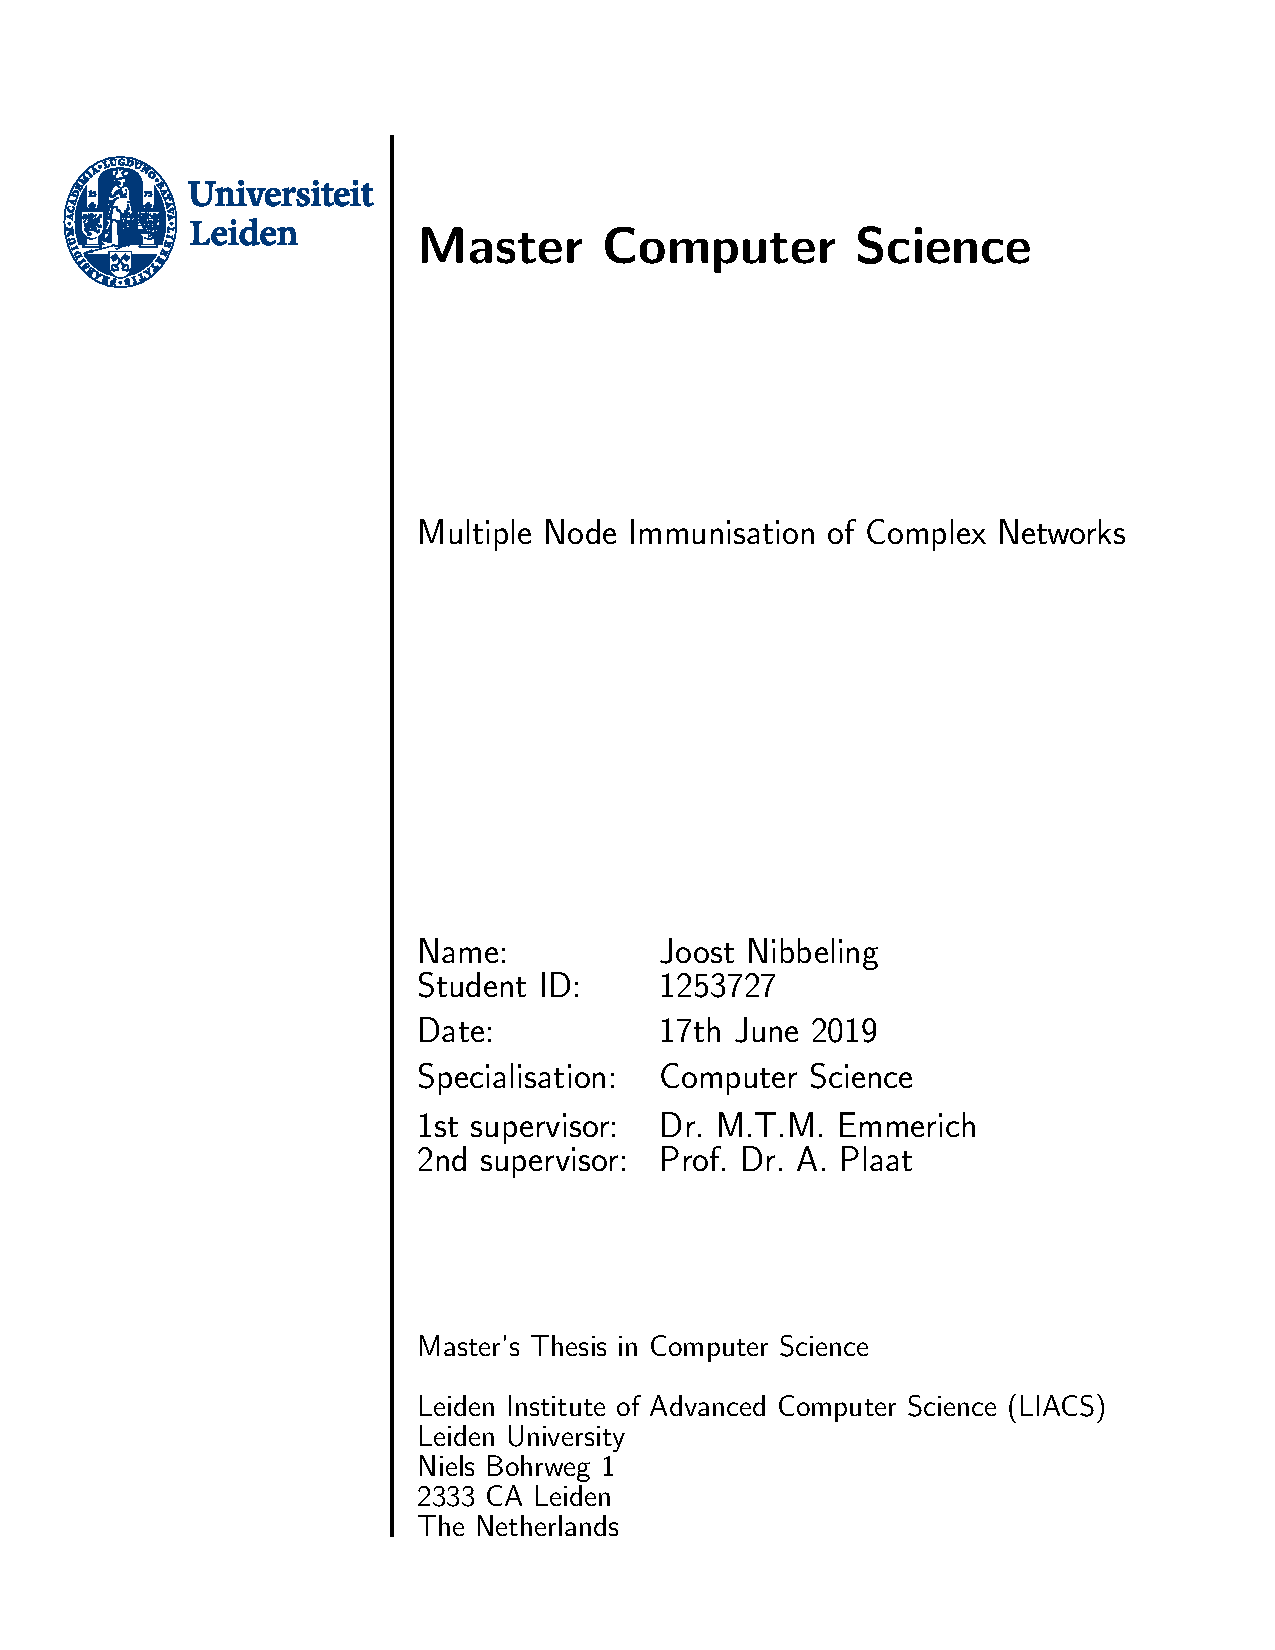
\includepdf[pages=-]{frontpage/frontpage.pdf}

\setcounter{page}{1}
\tableofcontents

\cleardoublepage

\addcontentsline{toc}{section}{Abstract}
\section*{Abstract}

Multiple node immunisation is the removal of nodes from a network to make it more robust against attacks by viruses. The problem is finding which nodes to remove to achieve the best possible immunisation. It has been found that the eigenvalue of the adjacency matrix of a network is a good measure for how susceptible it is to virus infection.

Therefore we compare different graph measures to the eigenvalues of all graphs with five nodes and of several randomly sampled larger graphs. This is to try and find correlations between these graph measures and the eigenvalue of a graph. The best found among these are the Shield-value from the NetShield algorithms and the average degree.

We also focus on two variations of the multi node immunisation problem. Solutions to both problems involve selecting nodes that when removed from the network maximise the eigen-drop: the difference in eigenvalue between the original and immunised network. The first problem variant requires the number of nodes $k$ to be removed to be known a priori. This problem has been proven to be NP-complete. We compare two different solutions. The first is the NetShield method. This method uses greedy approximation of a function that approximates the eigen-drop. The second uses a genetic algorithm meta-heuristic. The results show that the GA can be competitive with the NetShield algorithm under certain circumstances, but under others the NetShield algorithm provides the better solutions. In addition to this we simulate virus infections with continuous time Markov chains to evaluate the usefulness of eigen-drop as a performance measure.

The second problem variant defines the problem as a multi-objective one. Here each node is assigned a cost function and there is a trade-off between immunisation and cost of a solution. Therefore, the goal is to approximate the Pareto front. To do this we extend the NetShield algorithm with an $\epsilon$-constraint. We compare the results with two genetic algorithms specifically designed for multi-objective problems: NSGA-II and SMS-EMOA. We show that the extended NetShield method is capable of finding better Pareto front approximations than the GAs when the number of vertices in the graphs increases beyond 100. 

\cleardoublepage

\section{Introduction}

The study of complex networks has received increased attention in recent years. Empirical research on the study of real life networks such as computer networks and social networks has shown that many of them share features. For instance these networks may be examples of both small world and scale free networks. Several textbooks have been written on both the theory and applications of complex networks. Examples are \cite{van2016random}, \cite{Draief} and \cite{thai2011handbook}.

For this thesis we focus on the subject of multiple node immunisation. This is the removal of nodes from a graph so that the graph is less vulnerable to infection. Node immunisation has many applications in real life scenarios. The graph may represent a computer network that is under attack by a virus and we may want to find the best subset of nodes that should be removed to stop the spread. Similarly, the network may represent of series of airports through which a real-world contagious virus is spreading. Which of the airports should then be quarantined to stop the spreading of the virus the most effectively? But there are also applications in other settings. For example a network of criminals in law enforcement. Which criminals should be targeted to break up the network most effectively?

For this we need some measure of vulnerability of a graph. Previous work has shown that under the SIS epidemiological model the maximum eigenvalue of a graph is a good measure \cite{chakrabarti2008epidemic} \cite{li2013epidemic}. Secondly, we need methods that find a set of nodes that if removed, maximises the difference between the new eigenvalue and the old one. For this Chen Chen et al. \cite{chen2016node} propose the NetShield algorithm that works by greedy optimisation of a function that approximates this difference. Maulana et al. \cite{maulana2017immunization} make use of a problem specific genetic algorithm that has competitive performance with the NetShield algorithm. We extend the experiments done in \cite{maulana2017immunization} to see if the results remain competitive with graphs sampled from two random graph models instead of only real world networks. As both methods focus on maximising the eigenvalue difference, we perform additional experiments with simulations of infections on the network in the test data set. The purpose is to verify how well the theoretical vulnerability measure translates to a more empirical approach. The simulations are done via a continuous time Markov chain.

Both methods introduced above determine the number of nodes to remove a prior. Initial research has also been done by \cite{maulana2017immunization} for a multi-objective approach to the problem with the use of multi-objective genetic algorithms. Here there is a cost measure defined for nodes in the graphs as a second objective in addition to the original eigen-drop objective. This leads to a trade-off between immunisation effort and effectiveness, meaning that a Pareto front needs to be approximated. For the main contribution of this theses, we extend the NetShield methods to be used for the multi-objective problem and compare the performance with that of the GAs. The results also lead to some more insights into the shape of the Pareto front.

In addition, we also compare the eigenvalues of graphs to some other graph measures. The goal is to see how a graph measure that may be more easily computed correlates with the vulnerability of the graph. This is done via full enumeration of all graphs of a small size and random sampling of graphs of a larger size.

\subsection{Research Questions}

The following research questions summarise what is discussed above.

\begin{enumerate}
    \item Can we find correlations between the eigenvalue and other graph measures and therefore assess the vulnerability of a graph with these other measures?
    \item How do the NetShield algorithms compare with the GA approach in  extended experiments?
    \item Do the solutions found by the NetShield algorithm and the GA translate to good solutions in a virus infection simulation via a continuous time Markov chain?
    \item Can the NetShield algorithm be extended to work for a multi-objective view of the node immunisation problem and how does it compare to GAs designed for multi-objective optimisation tasks? Is it possible to combine the approaches?
    \item Does the Pareto front for the multi-objective node immunisation problem have a particular shape?
\end{enumerate}

\cleardoublepage

\section{Definitions}

This section contains a description of different epidemic models. This is followed by the definition of a graph and the notions following this about the eigenvalue of a graph.

\subsection{Epidemic models}

Research into the spread and behaviour of infections is an entire field of research on its own called \emph{epidemiology}. The spread of infections is a complicated process. To simplify the mathematical modelling of this process, compartmental models have been designed. In these models, the population is divided into several compartments or states. This discussion will focus on three of them. The first compartment is those denoted with S and contains the subset of nodes which are susceptible. Individuals in this compartment may be infected at some later point. The second comprises those who are infected. This compartment is denoted with I. The last state discussed here is denoted with R. In this compartment are the nodes which have recovered from the infection. These compartments gives rise to the following three models.


\begin{itemize}
\item SI model: In this model recovery is not possible. Individuals in the susceptible compartment may at some point in time move to the infected compartment. Once there, they will remain there indefinitely.
\item SIS model: In this model recovery is possible. At some point in time an infected individual may move to the susceptible state. There is no immunity after infection and after some time an individual may become infected again. Examples of such infections are the common cold or influenza.
\item SIR model: In this model, infected individuals move to the recovered compartment after some time. From this compartment, they can no longer return to a susceptible state. This can be used to models infections that cause long term immunisation after recovery. Examples of such infections are measles, rubella and mumps. Alternatively, this model can also be used to include individuals dying from the infection, after which they naturally can not get infected again.
\end{itemize}

It is possible to extend these models with more compartments and transitions, however such models will not be discussed here. For this thesis we will focus on the SIS model. This is combined with a simulation based on continuous time Markov chains. This simulation will be explained in a later chapter.


\subsection{Graphs and eigenvalue}

All algorithms described in the later chapters work on a structure called a network or graph. It is defined below.

\theoremstyle{definition}
\begin{definition}{Graph}
A network or graph $G=(V,E)$ consists of a set of nodes or vertices $V = \{v_1, v_2 ... v_n\}$ and a set of edges $E \subseteq V \times V$
\end{definition}

A graph is a set of objects in $V$ that are related to each other. These relations are modelled as edges. They are the pairs in $E$. Graphs can be directed or undirected. Here we focus only on undirected graphs. This means that the pairs in $E$ are unordered. Edges and nodes can also have weights. We only consider weights for the vertices for the multi-objective immunisation problem. Here the weights represent the costs. The edges are always unweighted.

A graph can be represented as a matrix called an adjacency matrix.

\begin{definition} An adjacency matrix $A$ of a graph is a matrix of size $N \times N$ with $N$ equal to the number of vertices in the graph. In case $(v_i, v_j) \in E$, then $A[i,j]$ is 1, otherwise $A[i,j]$ is 0
\end{definition}

The technique of representing a graph as a matrix also allows for eigen-decomposition of the matrix. This makes it possible to compute the maximum eigenvalue of a graph. This eigenvalue will be denoted with $\lambda$. With $\lambda$ the concept op eigen-drop can be defined.

\begin{definition}
Given a graph $G=(V,E)$ and a set of nodes $S \subseteq V$, the nodes in $S$ and edges attached to these nodes can be removed from $G$. This gives rise to the new graph $G'$ with a perturbed adjacency matrix \footnote{The perturbed matrix can be created by either setting the columns and rows corresponding to the selected nodes to zero or by completely removing them. Both matrices will yield the same $\lambda$.}. This new graph has a new first eigenvalue $\lambda'$. The eigen-drop $\Delta\lambda$ is defined as the difference between the two: $\Delta\lambda = \lambda - \lambda'$
\end{definition}

The reason for using $\Delta\lambda$ as a measure is because under the SIS epidemic model, this value is related to the epidemic threshold of a graph $\tau = 1/\lambda$ \cite{chakrabarti2008epidemic} \cite{li2013epidemic}. The epidemic threshold determines if a virus evaporates from a network or if it invades it. It is inversely proportional to $\lambda$. Therefore $\lambda$' of the new graph should be minimised. This is equivalent to maximising $\Delta\lambda$.

Finally there is the notion of the eigen-score. The eigen-score important to the NetShield and GA design.

\begin{definition}
The first eigenvalue $\lambda$ of a graph $G = (V,E)$ has a corresponding eigenvector $u$. The eigen-score of a node $v_i \in V$  is the corresponding component in the eigenvector $u_i$, $i=1,..,|V|$
\end{definition}

\cleardoublepage

\section{Relationship Between Maximum Eigenvalue and Other Graph Measures}

In this section the relationship between the maximum eigenvalue and several other graph measure is examined. The goal is to see if these other graph measures may also be some indication of the vulnerability of a graph. 
For this the graph measures have been plotted against the eigenvalue. The Pearson correlation coefficient has also been computed. The results are shown in Table \ref{tbl:pcc}. This has been done for graphs with two different number of vertices. For the first set, all possible undirected graphs with 5 vertices have been measured, for a total number of 1024 graphs. For the second set, undirected graphs with 30 vertices have been measured. As the number of possible graphs increases exponentially with the number of vertices, measuring all graphs with 30 vertices is not possible. Therefore 100000 graphs have been uniformly sampled.  
The graphs used in this section are undirected and unweighted. This means that the adjacency matrices are square symmetric matrices of which all elements are either 0 or 1. \cite{walker2008lower} gives several lower bounds for the maximum eigenvalue of symmetric matrices. The least accurate of these is the sum of all elements of the matrix divided by the number of rows. Therefore, all graphs here will have a maximum eigenvalue that is larger or equal to zero.

\begin{table}
\begin{center}
	\begin{tabular} { | l | l | l | }
	 \hline
	 Measure & V=5 & V=30 \\ 
	 \hline
	 Average betweenness & -0.15 & -0.98 \\
	 Average degree & 0.97 & 0.99 \\
	 Average path length & -0.77 & -0.98 \\
	 Number of cliques & 0.95 & 0.94 \\
	 Global clustering coefficient & 0.78 & 0.94 \\
	 Shield-value & 1.0 & 1.0 \\
	 \hline	 
\end{tabular}
	\caption{Pearson correlation coefficient with the eigenvalue for every tested measure for full enumeration of graphs with 5 vertices and Monte Carlo sampling of 100000 graphs with 30 vertices.}
	\label{tbl:pcc}
\end{center}
\end{table}

\subsection{Average Betweenness}

The betweenness centrality of a node $v$ is how many of the shortest paths in a graph go through that node. In this section the eigenvalue is compared to the average betweenness of all nodes in a network. There appears to exist an inverse correlation between average betweenness and a higher eigenvalue, at least when the number of vertices is sufficiently large. A slight correlation is visible in the left graph of Figure \ref{fig:measure_ab}. There is also a relatively small correlation coefficient in the table. The correlation shows much stronger in the right graph of the figure and the large negative correlation coefficient in the table. This correlation may exists because a vertex with a high betweenness may function as some sort of bottleneck, preventing some spread of the virus.

There are exceptions where this correlation does not show. These exceptions are shown more clearly for smaller graphs with fives nodes. They tend to occur in case many shortest paths are of length one and/or there exist many disjoint parts. This means no or few shortest paths cross through another vertex, resulting in low betweenness. This is most evident at the average betweenness of zero in the left graph. These are graphs in which all nodes are either part of a fully connected component or completely isolated. At the maximum eigenvalue of 4 is the fully connected graph. Then every time if a single node were to be isolated, the eigenvalue would drop by 1. This results in the evenly distributed points over the eigenvalue axis. This also creates the situation where both the fully disconnected and fully connected graph have the same betweenness but the largest difference in eigenvalue. The ratio of such exceptions appears to diminish when the number of vertices is increased. This results in the right graph of Figure \ref{fig:measure_ab} showing the correlation more strongly.

\begin{figure}[h!]
  \centering
    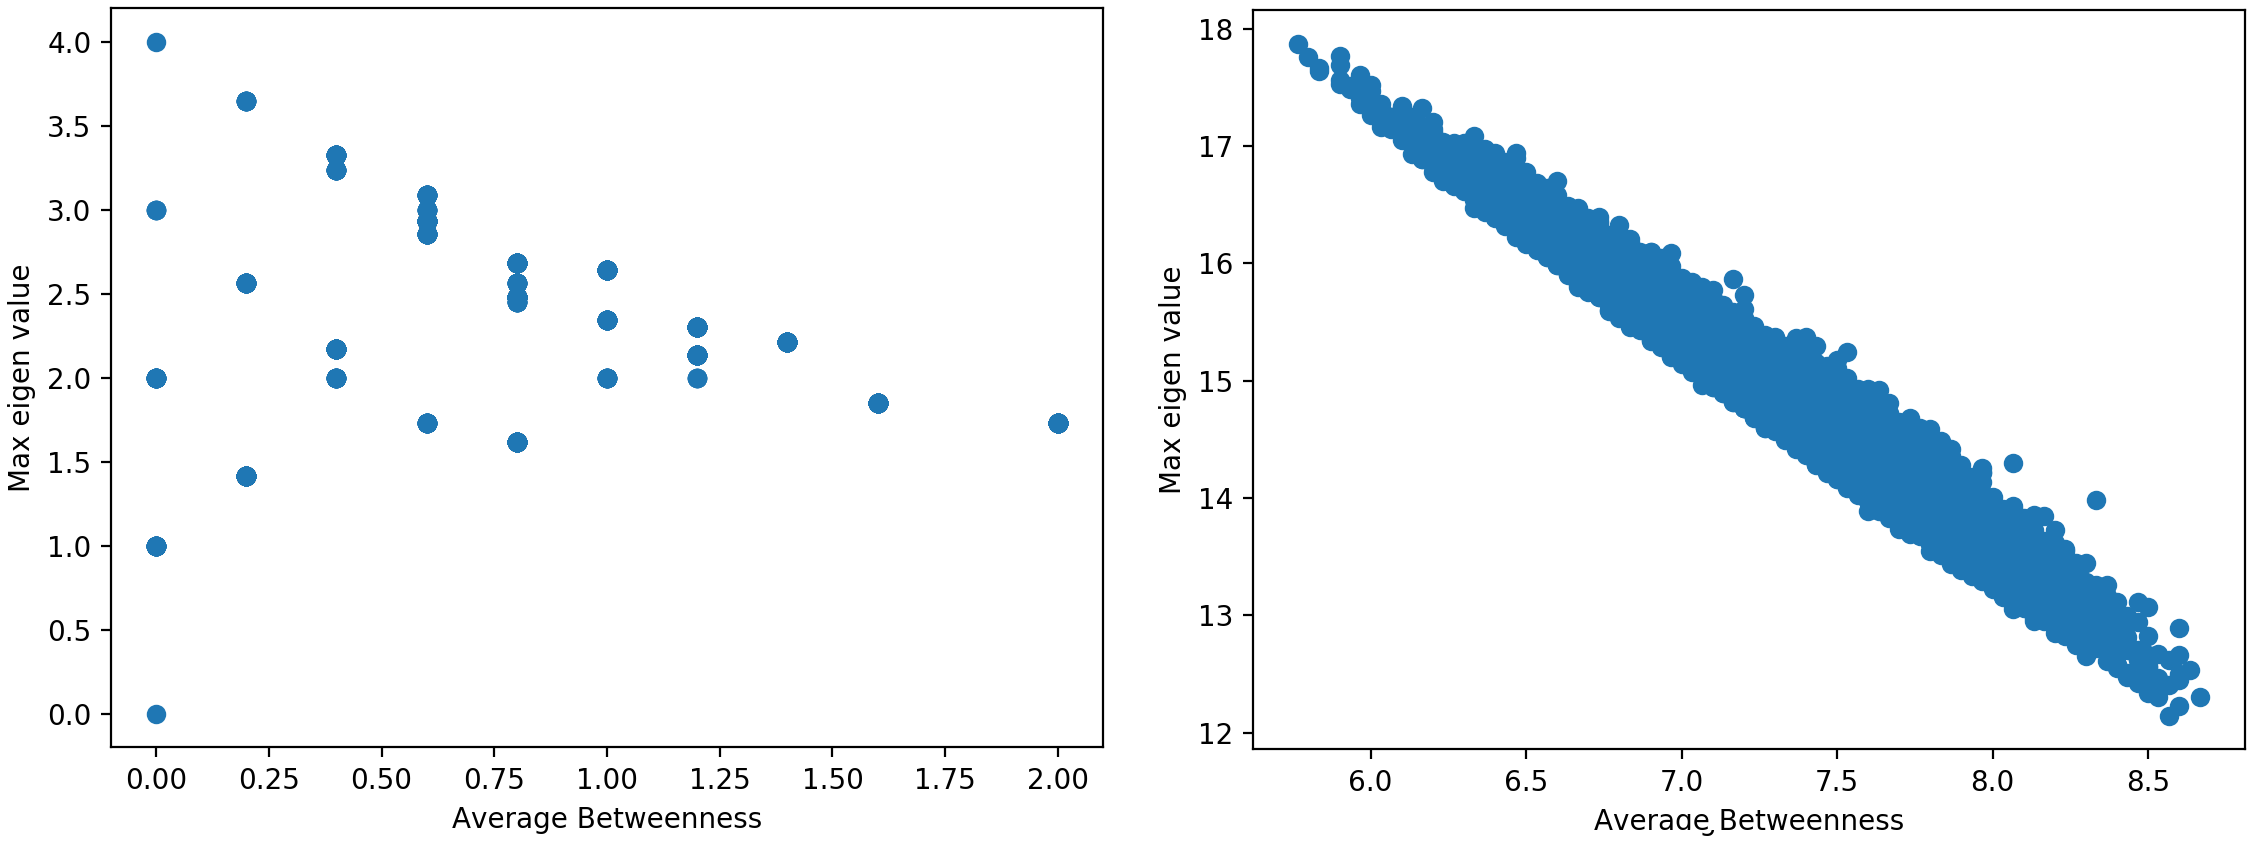
\includegraphics[width=1\textwidth]{results_graph_measures/Average_Betweenness_c}

  \caption{Average betweenness plotted against eigenvalue. Left: full enumeration for 5 vertices. Right: Monte Carlo sampling}
  \label{fig:measure_ab}
\end{figure}

\subsection{Average Degree}

Both plots in Figure \ref{fig:measure_ad} and the correlation coefficients in Table \ref{tbl:pcc} show strong positive correlation between average degree of the vertices with the eigenscore. A higher average degree means that there are more connections, so it would be intuitive that it would then be easier for an infection to spread through the graph. The graphs do show that there exist ranges of graphs with different eigenvalues for some average degrees. This is clearer in the left graph of the figure. These ranges can partially overlap when moving to higher or lower average degrees. This is also shown in the correlation coefficients, which shows that the average degree and eigenvalue is not completely correlated. So while the average degree can be an indication for the eigenvalue expected from a graph, there are more structural properties to a graph that influence this that an average degree measure can capture on its own.


\begin{figure}[h!]
  \centering
    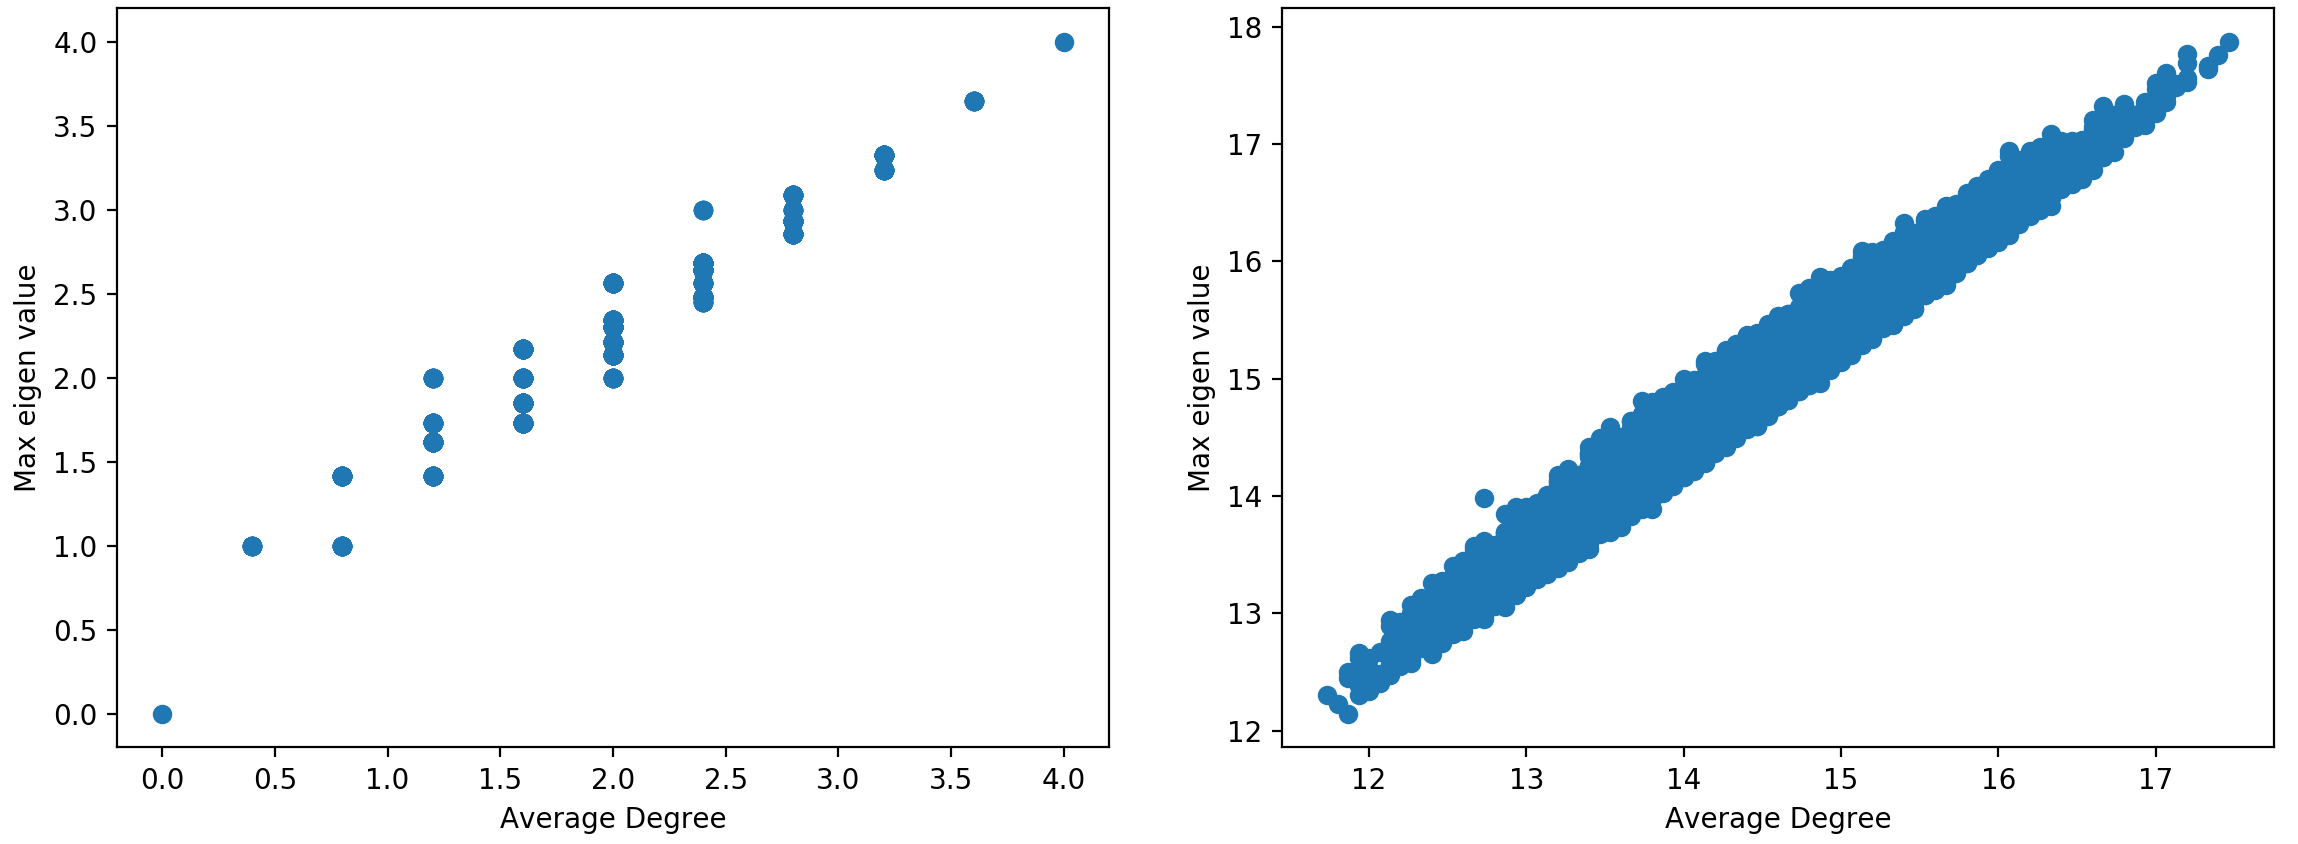
\includegraphics[width=1\textwidth]{results_graph_measures/Average_Degree_c}

  \caption{Average degree plotted against eigenvalue. Left: full enumeration for 5 vertices. Right: Monte Carlo sampling}
  \label{fig:measure_ad}
\end{figure}

\subsection{Average path length}

For the average path length a decision needs to be made about how to handle disconnected components. Here we choose to add a path of length $|V|$ between every pair of unconnected vertices. This choice is made because a large average path intuitively implies that it is more difficult for a virus to spread: it has to pass through many nodes. Disconnected components make it impossible for a virus to fully infect the entire graph when the virus only exist in not all of the components. So by that reasoning disconnected components should add to the average path length.

The graphs in Figure \ref{fig:measure_apl} and the correlation coefficients in Table \ref{tbl:pcc} show that there exists a negative linear correlation between average path length and eigenvalue. Just like with the average betweenness the correlation appears to be stronger for graphs with a larger number of vertices. The graph on the left of Figure \ref{fig:measure_apl} of fully enumerated smaller graphs with five vertices shows an odd spread that explains the lesser correlation. Initially the eigenvalue drops when the average path length increases. But then at an average path length of around 2.5, the eigenvalue jumps back up again. This is the result of graphs that consist of disconnected components, but with low average path length within these components. The most prominent of these being the point at approximately (2.5, 3.0). At this point are graphs with four vertices forming a complete graph, and a single disconnected vertex. This single isolated vertex explains the high average path length. But within this component the vulnerability to virus infection is high. This is captured properly by the eigenvalue measure.


\begin{figure}[h!]
  \centering
    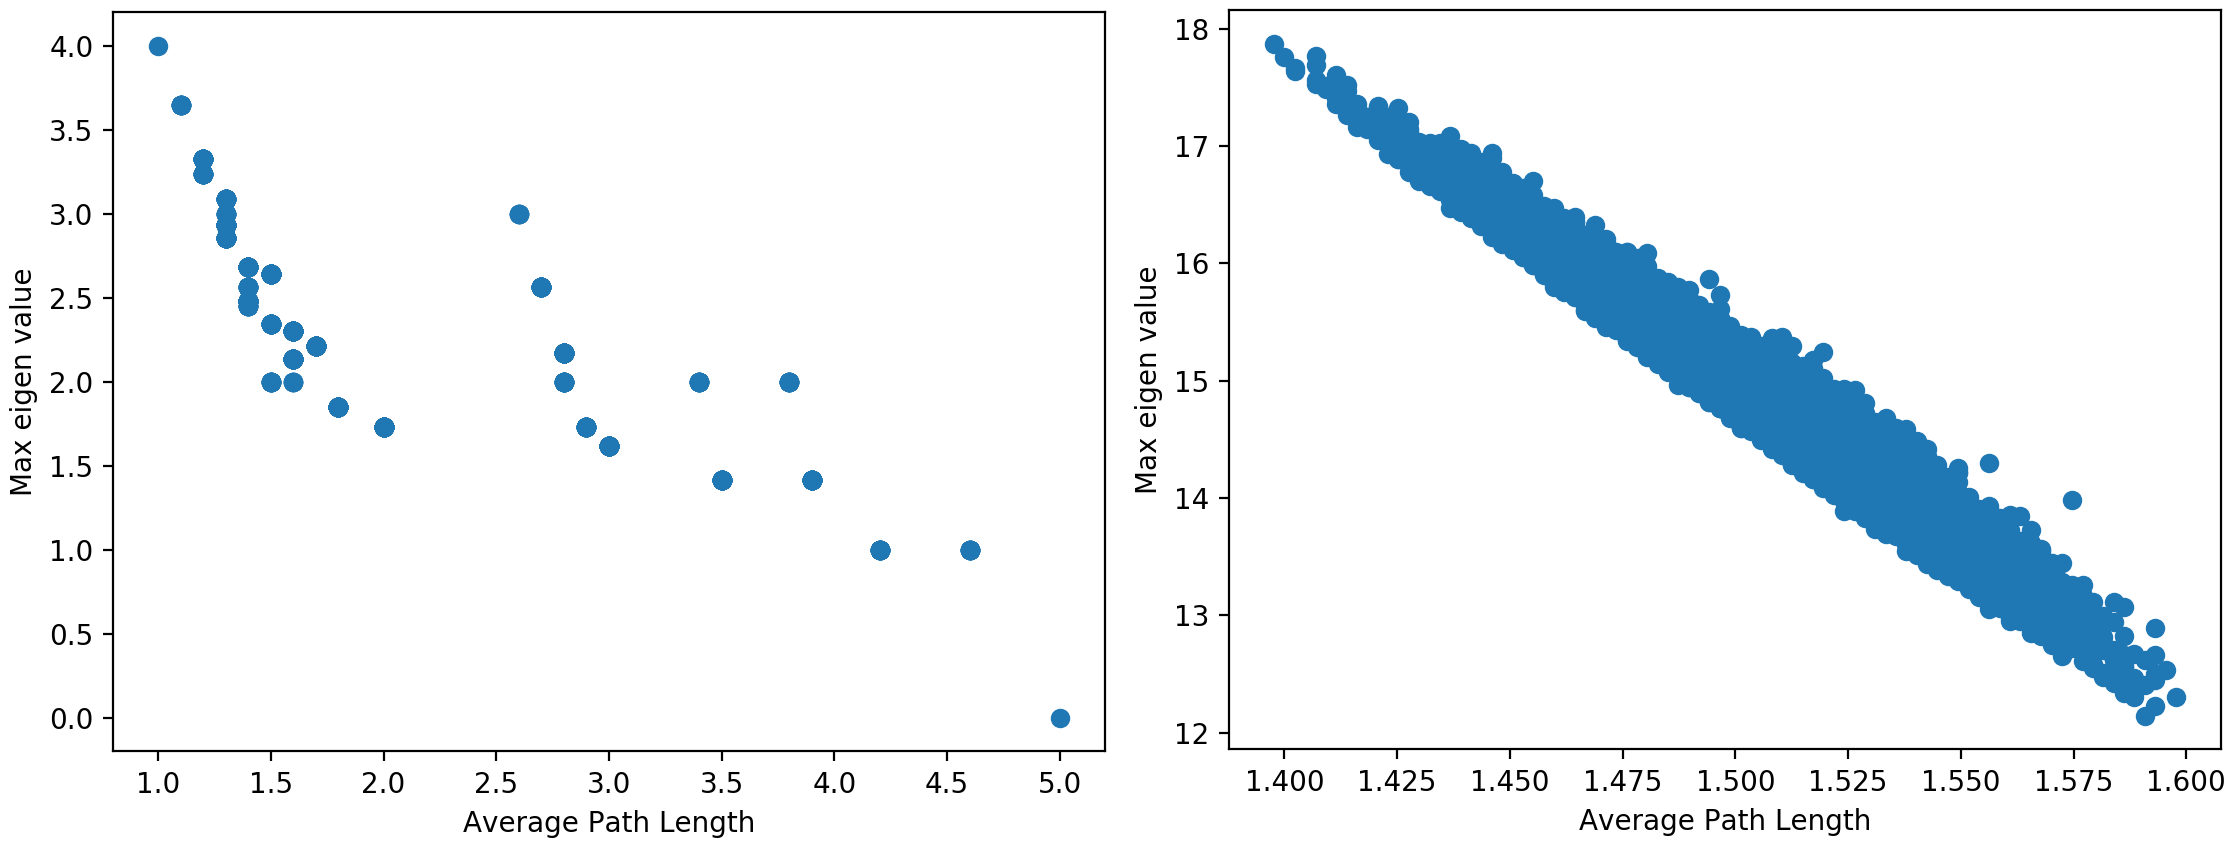
\includegraphics[width=1\textwidth]{results_graph_measures/Average_Path_Length_c}

  \caption{Average path length plotted against eigenvalue. Left: full enumeration for 5 vertices. Right: Monte Carlo sampling}
  \label{fig:measure_apl}
\end{figure}

\subsection{Number of Cliques}

There is a positive correlation between number of cliques and the eigenvalue as shown by Figure \ref{fig:measure_nql} and Table \ref{tbl:pcc}. As a clique is a set of vertices that are all connected to each other, it intuitively seems reasonable that a larger number of cliques would mean that infections could spread more easily. Although as with the average degree and the average path length, there is appears to be a range in which the points fall, again indicating that this metric does not fully correspond with the eigenvalue metric. Also as finding the total number of cliques still grows exponentially with regards to the number of input vertices, it is still computationally unfeasible to find all of them for larger graphs. 
Finally, while the previous graphs show the measures scaling mostly linearly with the eigenvalue, this is not the case here. When the number of cliques increases, the eigenvalue increases less steeply. Furthermore, when looking at the right graph, the range appears to expand in the middle. This results in this measure being the only one where the Pearson correlation coefficient decreases slightly when increasing the number of vertices.

\begin{figure}[h!]
  \centering
    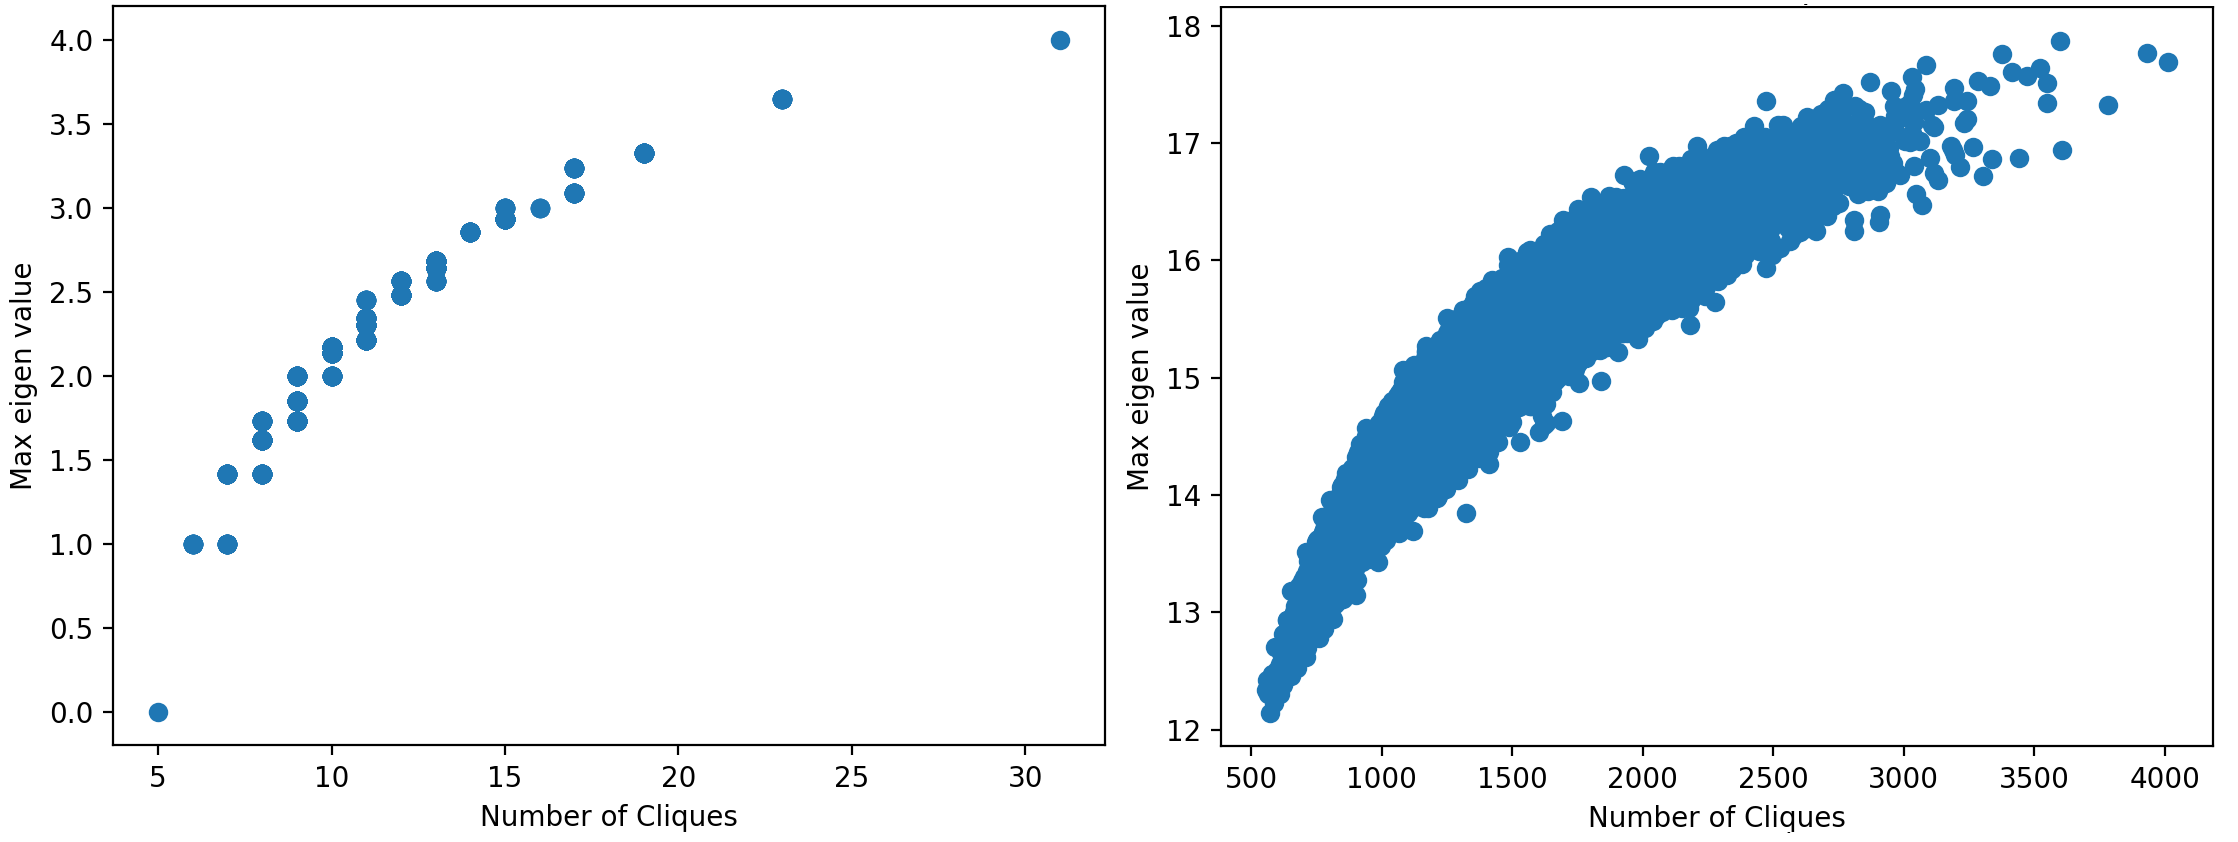
\includegraphics[width=1\textwidth]{results_graph_measures/Number_of_Cliques_c}

  \caption{Number of cliques plotted against eigenvalue. Left: full enumeration for 5 vertices. Right: Monte Carlo sampling}
  \label{fig:measure_nql}
\end{figure}

\subsection{Global Clustering Coefficient}

The global clustering coefficient is the number of closed triplets divided by all triplets. It would seem intuitive that if the number of closed triplets is high, an infection would spread more easily through a network. The left graph in Figure \ref{fig:measure_gcc} and Table \ref{tbl:pcc} show some positive correlation between eigenvalue and the global clustering coefficient. This correlation becomes stronger when moving to larger graphs as both the right graph and the Pearson correlation coefficients show. 

There is a group of outliers at the bottom left of the left graph in Figure \ref{fig:measure_gcc}. These are graphs where there are simply no closed triplets, so the global clustering coefficient is zero for these graphs. However, a closed triplet is unnecessary for an infection to spread, any edge will do. This means there are some graphs with different eigenvalues and therefore different vulnerability, but that do have the same global clustering coefficient. The same is also a probable cause for the other outliers. They may be less or more vulnerable to infection, but all have relatively few closed triplets. 

\begin{figure}[h!]
  \centering
    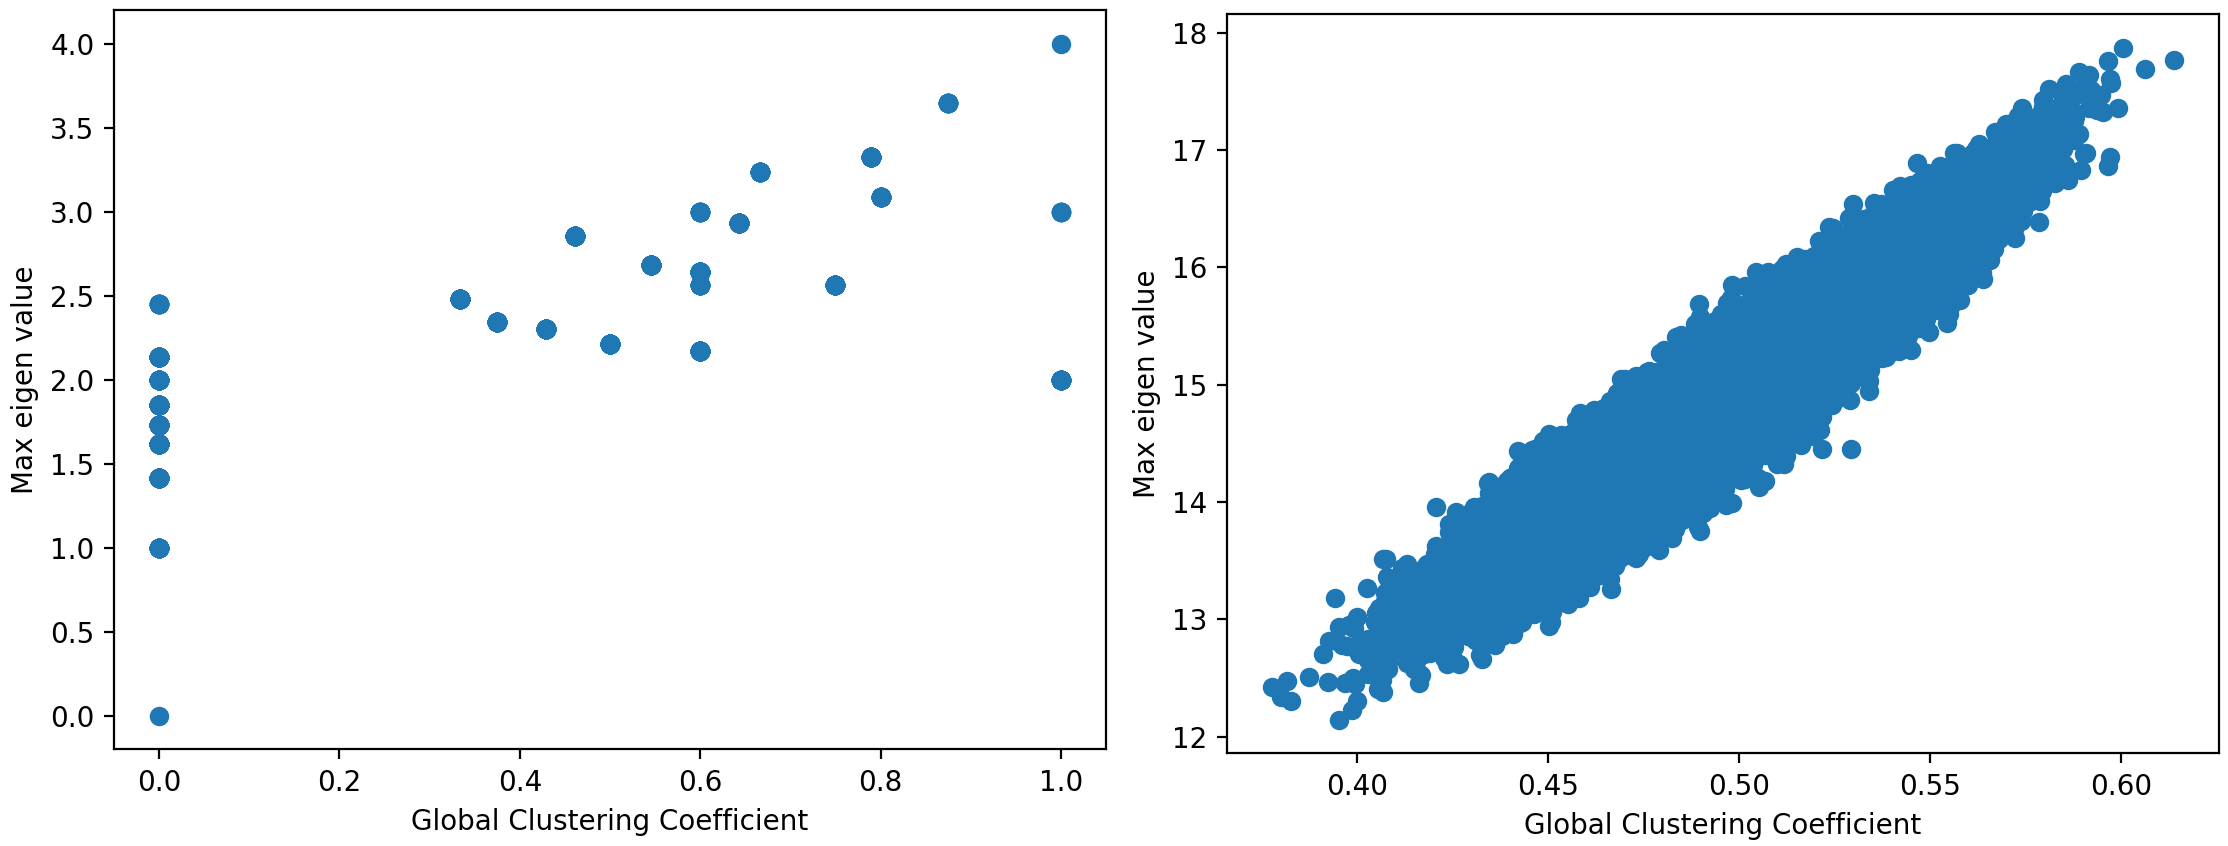
\includegraphics[width=1\textwidth]{results_graph_measures/Global_Clustering_Coefficient_c}

  \caption{Global clustering coefficient plotted against eigenvalue. Left: full enumeration for 5 vertices. Right: Monte Carlo sampling}
  \label{fig:measure_gcc}
\end{figure}

\subsection{Shield-value}

The final measure examined is the Shield-value. This measure is used in the NetShield and NetShield+ algorithms. \cite{chen2016node}. It uses the maximum eigenvalue and corresponding eigenvector to compute a so called Shield-value over a set of selected node. This Shield-value approximates how much the maximum eigenvalue of the graph would drop if all selected vertices were to be isolated. In this section the Shield-value is computed over all the nodes in the vertex. It should therefore approximate the eigenvalue of the graph, as removing all the vertices would drop the eigenvalue to zero.

The results are shown in Figure \ref{fig:measure_sv} and the last row in Table \ref{tbl:pcc}. This shows that there is a perfect linear correlation between eigenvalue and Shield-value. This is not unexpected, as the Shield-value is directly computed from the eigenvalue. This also indicates that the measure should work well for what it is designed for. Both graphs do however show that the Shield-value always overestimates the actual eigenvalue, with the exception of the fully disconnected graph. This is shown in the leftmost extreme of the left graph of Figure \ref{fig:measure_sv}. Both eigenvalue and Shield-value are zero.


\begin{figure}[h!]
  \centering
    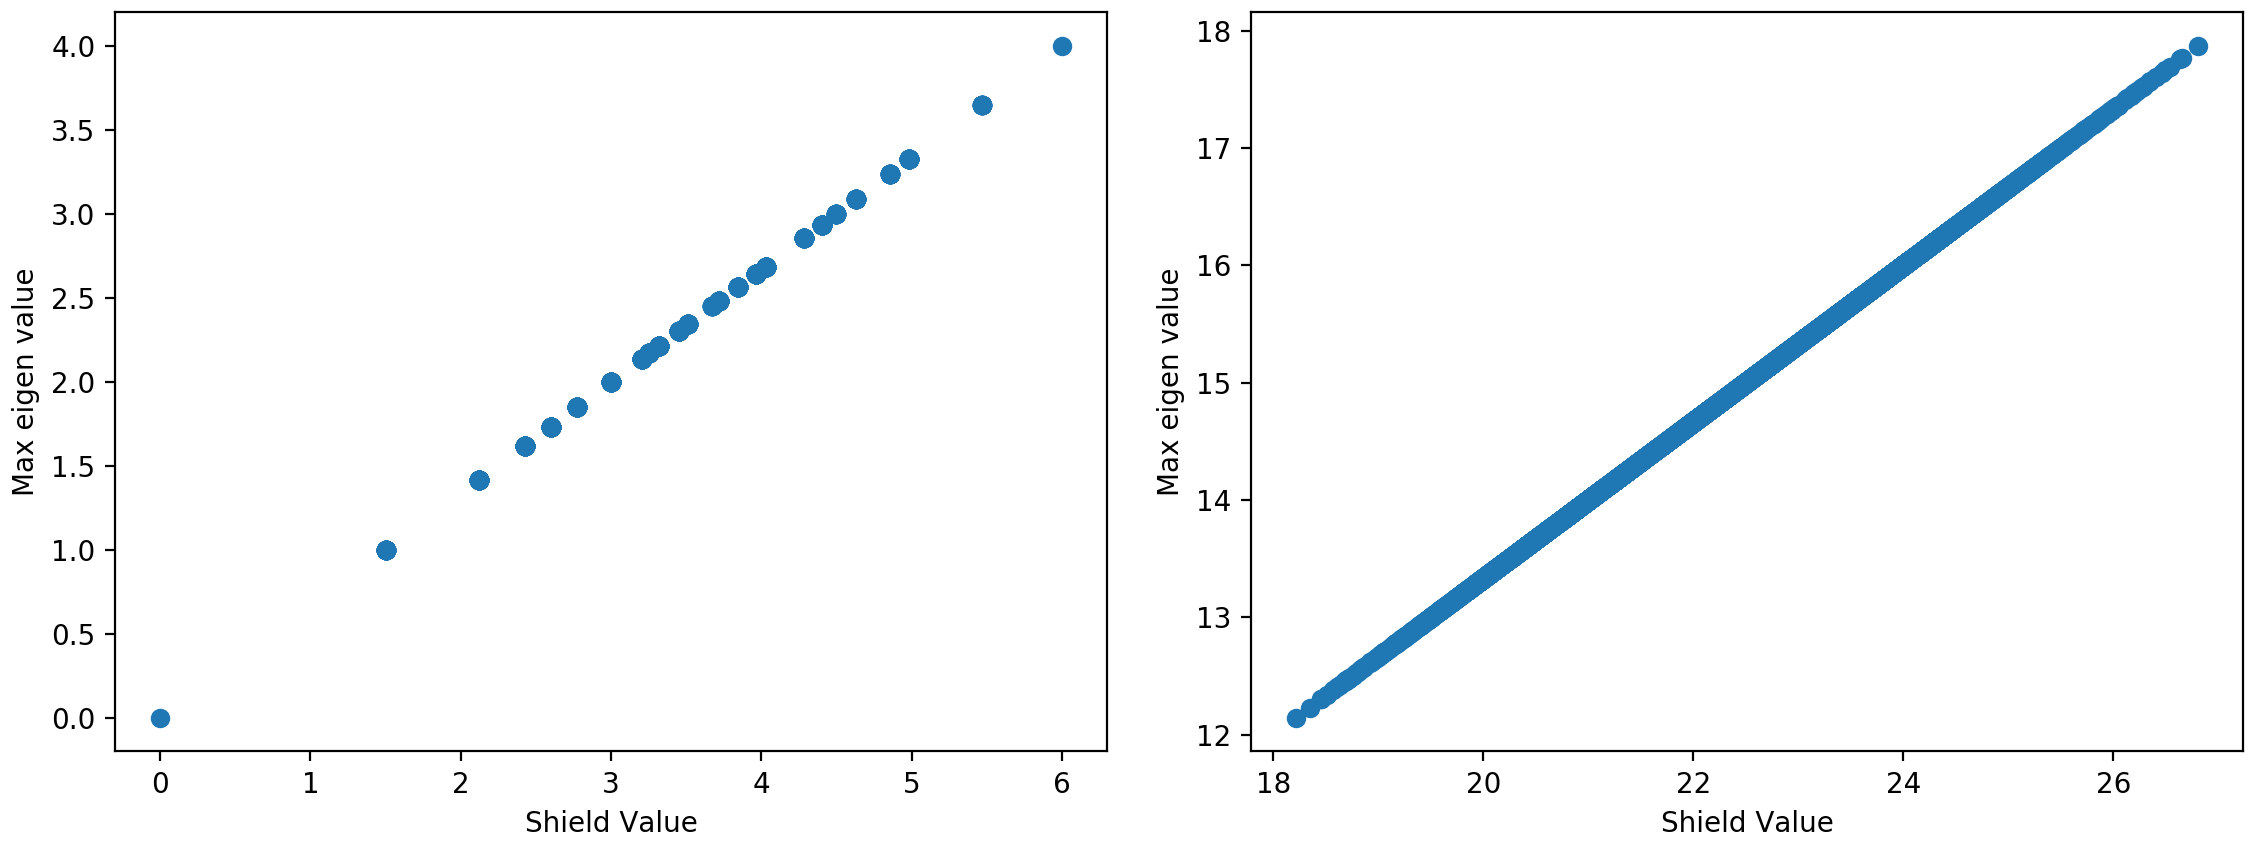
\includegraphics[width=1\textwidth]{results_graph_measures/Shield_Value_c}

  \caption{Shield-value plotted against eigenvalue. Left: full enumeration for 5 vertices. Right: Monte Carlo sampling}
  \label{fig:measure_sv}
\end{figure}

\cleardoublepage

\section{$k$-Node Immunisation}

The definition of the $k$-node immunisation problem is as follows.

\begin{definition}
Given a graph $G=(V,E)$ and $k \in\{1,\dots,|V|\}$, determine $S \subseteq V$ and $|S| = k$ such that removal of these nodes from $G$ maximises the eigen-drop $\Delta\lambda$
\end{definition}

This problem has been proven to be NP-Complete by Chen Chen et al \cite{chen2016node}. Therefore, two different approaches to solving such a problem are described in the next section. 

\subsection{Shield-value and NetShield algorithm}

To solve the problem of finding a subset which maximises the eigen-drop, the NetShield and NetShield+ algorithms have been designed by Chen Chen et al \cite{chen2016node}. Instead of working directly on the eigen-drop, these algorithms use a function that computes an approximation of the eigen-drop given a set of nodes that are to be isolated. This approximation is called the Shield-value. The definition of the Shield-value is given below.

\begin{equation}
    Sv(S) = \sum_{i \in S} 2 \lambda u_{i}^{2} - \sum_{i,j \in S} 2 u_{i}u_{j}A_{ij}
\end{equation}

In this equation A is the adjacency matrix of the network to be immunised. $\lambda$ is the first eigenvalue of the matrix $A$ and $u$ the corresponding eigenvector. The intuition is that a set of vertices has a high Shield-value if each node \textit{i} within the set has a high eigen-score. At the same time nodes should also be distant to each other, especially if they have high eigen-scores. This means that $A_{ij}$ should be small or zero if both node $i$ and $j$ are in the solution set.

To optimise this Shield-value, the NetShield algorithm has been designed. It is described in Algorithm~\ref{alg:netshield}. It uses a greedy approximation method to maximise the Shield-value. Initially, in lines 1-3 the first eigenvalue and corresponding eigenvector are computed and the solution set is initialised to be empty. Lines 4-6 compute the Shield-values of each individual node. Then in lines 7-20, the solution set of \textit{k} vertices is computed. Lines 8-17 compute what the increase in Shield-value would be if any not yet added vertices were to be added to the solution set. Then in lines 18-19, the vertex that would increase the Shield-value the most is added to the solution set.

For the Shield-value to be a good approximation of the eigen-drop, \cite{chen2016node} states that $k \leq d/8$ should hold. Here $d$ is the maximum degree of the network. To handle the problem where the number of vertices to be removed is too large, the NetShield+ algorithm has been designed. It is described in Algorithm \ref{alg:netshield_plus}. In addition to requiring the number of vertices to be removed, the NetShield+ algorithm also requires a batch size $b$. Then instead of removing $k$ vertices at once, the NetShield algorithm is performed $\lceil k/b \rceil$ times with at most $b$ vertices removed at each step. After each iteration, the vertices selected are removed from the adjacency matrix. Then the next call to the NetShield algorithm uses the new perturbed matrix instead. As a consequence $\lambda$ and the eigen-scores will be recomputed for the new matrix. This way the NetShield+ method can trade-off computational time with accuracy of the result.

The Shield-value function is a submodular function \cite{chen2016node}. This means that the greedy approximation algorithm used by NetShield is guaranteed to be at most $1-1/e$ off from the maximum. As the Shield-value is also a quadratic function, it is possible to define the optimisation of the Shield-value function as a quadratic integer program.

\begin{equation}
\begin{gathered}
\text{Given an adjacency matrix A of size $m*m$, its first eigenvalue $\lambda$ and its first eigenvector u:}\\
f_{1}(x) = \sum_{i=1}^{m} 2 \lambda  u_{i}^{2} x_{i} - \sum_{i=1}^{m} \sum_{j=i+1}^{m} 2 u_{i} u_{j} A_{ij} x_{i} x_{j} \to \max \\
\text{Subject to:}\\
f_{2}(x) = \sum_{i=1}^{m} x_{i} = k\\
x = \{0,1\}^{m}
\end{gathered}
\end{equation}

Here the solution is defined as a binary decision vector $x$. If the component $x_{i}$ is one, this means the node has been selected. In case $x_{i}$ is zero, the node is not selected. The objective function is the Shield-value function, but defined in terms of the binary decision vector. The constraint fixes the maximum of selected vertices to $k$. Inputting this quadratic program in a solver, may result in a better solution than a greedy approximation as these solvers typically employ a branch and bound based method.

A quadratic program solver can also be used inside of the NetShield+ algorithm. Instead of multiple greedy approximations with a smaller batch size $b$, multiple quadratic programs with a modified constraint that fixes the maximum number of selected vertices to $b$ can be solved. This may lead to more accurate results. However, if the batch size is set to 1 the second quadratic part of the Shield-value function will always evaluate to zero. Furthermore only a single vertex may be selected. This results in a trivially solvable linear integer program: the vertex with the highest eigen-score should be selected. The NetShield+ algorithm will in this case also select the same vertex. This means that in case of a batch size of one, both the NetShield approximation and the quadratic program method will always give the same solution.

\begin{algorithm}
  \caption{NetShield
    \label{alg:netshield}}
  \begin{algorithmic}[1]
    \Require{The adjacency matrix $A$ and an integer $k$}
    \Ensure{a set $S$ with $k$ nodes}
    
    \Statex
    \Let{$\lambda$}{First eigenvalue of $A$}
    \Let{$u$}{Corresponding eigenvector of $\lambda$}
    \Let{$S$}{$\emptyset$}
    \For{$j$ $\leftarrow$ 1 to $n$}
        \Let{$v_j$}{2 * $\lambda$ $-$ $A_{jj}$ $*$ $u_j^2$}
    \EndFor
    
     \For{1 to \textit{k}}
        \Let{$B$}{$A$(:,$S$)}
        \Let{$b$}{$B$ * $u$($S$) }
        \For{\textit{j} $\leftarrow$ 1 to \textit{n}}
        
        \If{\textit{j} $\in$ \textit{S}}
            \Let{score$_j$}{$-1$}
        \Else
            \Let{score$_j$}{$v_j$ $-$ 2 $*$ $b_j$ $*$ $u_j$}
        \EndIf
        \EndFor
        \Let{\textit{i}}{argmax(score)}
        \Let{\textit{S}}{\textit{S} $\cup$ \{\textit{i}\}}
    \EndFor
    \State \Return{\textit{S}}
  \end{algorithmic}
\end{algorithm}


\begin{algorithm}
  \caption{NetShield+
    \label{alg:netshield_plus}}
  \begin{algorithmic}[1]
    \Require{The adjacency matrix $A$ and two integers $k$ and $b$}
    \Ensure{a set \textit{S} with \textit{k} nodes}
    
    \Statex
    \Let{$S$}{$\emptyset$}
    \Let{iterations}{$\lfloor k/b \rfloor$}
    \For{$j$ $\leftarrow$ 1 to iterations}
        \Let{$S'$}{\textit{NetShield}($A$, $b$)}
        \Let{$S$}{$S$ $\cup$ $S'$}
        \Let{$A$}{DeleteNodes($A$, $S'$)}
    \EndFor
    \If{$k$ $>$ iterations $*$ $b$}
        \Let{$S'$}{\textit{NetShield}($A$, $b$)}
        \Let{$S$}{$S$ $\cup$ $S'$}
    \EndIf
    \State \Return{$S$}
  \end{algorithmic}
\end{algorithm}

\subsection{Genetic Algorithm}

The NetShield algorithm does not work on eigen-drop directly, but is a greedy algorithm that uses the Shield-value to approximate a good solution. This means that a better solution can exist that the NetShield algorithm cannot find. A genetic algorithm is a metaheuristic that samples from the search space in an efficient way. Genetic algorithms are inspired by the process of natural evolution. Such a method can be made to work directly on the eigen-drop and can consider more solutions that a greedy algorithm would. Because of this, a genetic algorithm may potentially result in better solutions. This section describes a genetic algorithm specifically designed for optimising the problem of eigen-drop by Maulana et al. ~\cite{maulana2017immunization}.

A genetic algorithm requires a population of solutions represented in some form and a fitness function to evaluate how good every individual solution is.
Here the fitness function to be maximised is the eigen-drop. The solutions are represented as a permutation of the integers $\{1..n\}$. The first $k$ nodes from the permutations are the nodes to be selected.

At the beginning a population of $\mu$ of solutions is initialised randomly. From this population the next generation is created via a process of parent selection, crossover and mutation. Crossover can occur with a probability of $p_c$. When this occurs, two parents are selected with scaled proportional selection. This means that parents with higher fitness are more likely to be selected for crossover. The crossover operator combines the selected parents, $p_1$ and $p_2$, into a new candidate solution $c$. The GA uses a problem specific crossover operator. The nodes $c[1:k]$ of the new solutions are chosen by taking the union of the nodes $p_1[1:k]$ and $p_2[1:k]$. If this union is larger than $k$, nodes are randomly discarded until a selection of nodes of size $k$ is reached. The nodes $c[k+1:n]$ are chosen by taking the complement of $\{1,..,n\}$ and $c[1:k]$. This way, the candidate solution remains a valid permutation of $\{1,..,n\}$ 

This newly created candidate is modified with the mutation operator. This mutation operator is also problem specific. It works with two mutation rates: $p_m^1$ and $p_m^2$. The first mutation rate is assigned to nodes with the top $k$ eigen-scores and the second to the other nodes. Then a single node is selected from $c[1:k]$ and from $c[k+1:n]$ with the above rates. The probability of choosing a node is computed by dividing the rate of the node by the sum of all rates of the nodes in the selection from which the node is chosen. These nodes are then switched. By choosing a higher rate $p_m^1$ than $p_m^2$, the search will be more focused on nodes with high eigen-score. This uses the intuition from the Shield-value that says that choosing nodes with high eigen-scores is more likely to result in a larger eigen-drop. 

This process continues until $\mu$ new solutions have been created. Then the $\mu$ solutions with the best fitness are chosen from both the new and old solutions. The chosen solutions form the population of the next generations. The GA stops when it reaches a set number of generations. In addition, this GA uses an early termination criterion. If the best fitness found does not improve for $k(n-k)$ generations, the GA stops immediately. The number $k(n-k)$ is used as it is proportional to the number of possible mutations in a single solution.

\subsection{Continuous Time Markov Chain Simulation}

Both the NetShield algorithms and the genetic algorithms work by selecting a subset of vertices that maximise the eigen-drop. This yields a good indicator for the vulnerability for large networks. It needs to be investigated if this is also true for smaller finite graphs. To this end a stochastic simulation of virus infection can be employed. We perform this simulation on all networks in the data set. The simulation method is the continuous time Markov chain (CTMC). The simulation is defined as a jump and hold system. At any particular point in time the system is in a certain state. This state is held for a period of time until an event occurs. During the event, the system jumps to the next state. The next state is solely dependent on the current state and is randomly chosen from a set of possible state transitions.

The epidemic model used for the infection process in the simulations is the SIS model. In this model vertices are initially set to the susceptible state after which a random node gets infected. After a vertex is infected, there is a chance that that the vertex will recover at a later time. When this happens, the vertex reverts to a susceptible state, meaning it is possible for the vertex to be infected again. Hence for this simulation, the full state of the system is which nodes are infected and which nodes are susceptible. This means that the complete state space has a size of $2^n$, where $n$ is the number of nodes in the network. During a state change of the system, the state of a single node is changed. A node is changed from susceptible to infected or vice versa. This means that from a state $i$ at most $n$ other states can potentially be reached.

During a state change, the system changes from state $i$ to state $j$. The rate $q_{ij}$ defines how likely it is for the state $i$ to transition into state $j$. If $q_{ij}$ is zero, it is impossible to reach state $j$ from state $i$. The rate $q_{ii}$ is the rate at which the system leaves the current state:

\begin{equation}
    q_{ii} = \sum_{j=1, j \neq i}^{N} q_{ij}
\end{equation}

The holding time until the next state change depends on this rate. The holding time is drawn from the exponential distribution with a mean of $1/q_{ii}$. In case $q_{ii}$ is zero, the holding time is infinite and the system will no longer transition to any subsequent state. This is the absorbing state.

For the infection simulation, the rates $q_{ij}$ depend on two parameters $\zeta$ and $\eta$. $\eta$ represents the contagiousness of the virus, $\zeta$ represents the recovery rate. During a state change to state $j$, a node $j$ will either become infected or vulnerable. The rate at which a node becomes infected is:

\begin{equation}
    q_{ij} = \textit{infected neighbours of j} * \eta
\end{equation}

The rate at which a node recovers is:

\begin{equation}
    q_{ij} = \zeta
\end{equation}

The probability of the system transitioning from state $i$ to state $j$, $p_{ij}$, depends on both the rates $q_{ij}$ and $q_{ii}$.

\begin{equation}
    p_{ij} = q_{ij} / q_{ii}
\end{equation}

All probabilities together form a probability distribution from which the next state is then sampled. At the start of the simulation, a single random node is infected. With the SIS epidemic model, the simulation will only reach the absorbing state when no nodes are infected anymore. This means the network has fully recovered. The full simulation is also described in pseudo code in Algorithm \ref{alg:CTMC}

Aside from the solutions found by the NetShield algorithms and the GA, two additional immunisation methods are also used to create solutions for simulation. The first method is to simply select $k$ random nodes. This to check if there is indeed a point to targeting eigen-drop instead of randomly removing nodes. The results from Section 3 show that the strongest correlation found is that between eigenvalue and average degree. The second method therefore removes the $k$ nodes with the highest degree to lower the average degree of the perturbed network as much as possible. This is to check if a comparatively much simpler solution than NetShield or a GA would suffice to get good results.

\begin{algorithm}
  \caption{CTMC
    \label{alg:CTMC}}
  \begin{algorithmic}[1]
    \Require{A graph G(V,E), infection rate $\eta$, recovery rate $\zeta$, maximum number of events}
    
    \Statex
    \Let{infection\_states}{Initialise all to SUSCEPTIBLE}
    \Let{infection\_states[random\_node]}{INFECTED}
    
    \While{not maximum events reached and not absorbing state reached}
        \ForAll{nodes $j$ of G}
            \If{infection\_states[node] is INFECTED}
                \Let{$q_{i}$[$j$]}{$\zeta$}
            \Else
                \Let{$q_{i}$[$j$]}{$\eta$ $*$ \# infected neighbours of $j$}
            \EndIf
        \EndFor
        \Let{$q_{ii}$}{ $\sum_{j=1, j \neq i}^{|V|} q_i[j]$}
            \If{$q_{ii}$ is 0}
                \State Absorbing state reached
            \Else
                \Let{$\Delta T$}{RandExp($1/q_{ii}$)}
                \State Wait($\Delta T$)
                
                \ForAll{$q_{ij}$ in $q_i$}
                    \Let{$p_i[j]$}{$q_{ij}/q_{ii}$}
                \EndFor
                \Let{selected\_node}{Sample($p_i$)}
                \If{infection\_states[selected\_node] is INFECTED}
                    \Let{infection\_states[selected\_node]}{SUSCEPTIBLE}
                \Else
                    \Let{infection\_states[selected\_node]}{INFECTED}
                \EndIf
            \EndIf
    \EndWhile
  \end{algorithmic}
\end{algorithm}

\subsection{Experiments and Results}

Three different sets of experiments have been run. The first section first describes the graphs in the test set. The second section focuses on the performance of the NetShield algorithm versus the optimising of the Shield-value with a quadratic program solver. The third section compares the performance of the GA against the NetShield+ algorithm. The final section shows the results of the CTMC simulations.

\subsubsection{Data set}

The test set contains eight different graphs. Six of these are medium sized graph from literature. The last two are sampled from two different random graph models. The networks with the number of nodes and edges are summarised in the appendix in section A.1. In addition all networks have also been visualised in the appendix in section A.2. In these visualisations, the nodes are scaled based on their degree.

\begin{itemize}
    \item Karate: This is a social network between members of a karate club at a university in the US in the 1970s \cite{zachary1977information}. It consists of 34 nodes. See Figure \ref{fig:karate}.
    \item Dolphins: A social network of frequent associations between dolphins living in a community of Doubtful Sound, New Zealand \cite{lusseau2003bottlenose}. It consists of 62 nodes. See Figure \ref{fig:dolphins}.
    \item USA: A graph of 27 of the most important airports in the USA. If there is a flight from one airport to another, they are connected by an edge. Data retrieved from \cite{usaref}. See Figure \ref{fig:USA}.
    \item Pandemic: Based on a board game in which a global virus outbreak is fought. The graph connects 27 cities in the world to each other \cite{pandemicref}. See Figure \ref{fig:pandemic}.
    \item Conference Day 1: Interactions between members of a conference on the first day. Only the largest connected components has been selected from this graph. Retrieved from \cite{confref}. See Figure \ref{fig:day1}
    \item Conference Day 3: Same as the above, except from the third day of the conference. See Figure \ref{fig:day3}
\end{itemize}

The first random graph model is the Erd\H{o}s-R\'enyi model. This model is defined with two different variations that have different input parameters. The first takes as input parameters the number of vertices and a probability. This is the probability that there is an edge between every pair of vertices. The second variant defines a number of vertices and a number of edges. Then with a uniform distribution one graph is chosen of all possible graphs with that number of vertices and edges. 

The second random graph model is the Barab\'asi-Albert model. Unlike the Erd\H{o}s-R\'enyi model this model creates a scale-free network. In such a network the degree distribution follows a power law: the fraction of nodes with a degree of $k$ is roughly proportional to $k^{-\tau}$ for some $\tau > 1$. This is largely independent of the actual size of the network. It is argued that many real life networks, such as the internet itself, are examples of scale-free networks. The model does this via a preferential attachment mechanism. The algorithm works by adding one node at a at a time. After a node is added, $m$ connections to other nodes are created from the just added node. The probability $p_i$ of choosing a node $i$ as the other end of the edge is given as follows: 

\begin{equation}
    p_i = \frac{k_i}{\sum_{j} k_j}
\end{equation}

In this formula $k_i$ denotes the degree of the vertex $i$. A vertex that already has many connections is therefore more likely to get even more. This ``rich gets richer"-scheme ensures that there will be a few large hub vertices to which many of the other vertices are attached. 

To make comparison between the Erd\H{o}s-R\'enyi graph and Barab\'asi-Albert graph as straightforward as possible, the parameters were set in such a way that for both models the sampled graphs have the same number of vertices and edges. In addition, they were also chosen so that the Erd\H{o}s-R\'enyi graph would likely be connected, because the Barab\'asi-Albert models always generates connected graphs. The Barab\'asi-Albert graph was generated with 100 vertices and $m$ was set to 3. The resulting graph has 294 edges. The Erd\H{o}s-R\'enyi graph was then created via the second definition to get the same number of edges and vertices. Erd\H{o}s-R\'enyi graphs were sampled until a network was created that was fully connected. The Erd\H{o}s-R\'enyi graph is visualised in Figure \ref{fig:erdosrenyi} and the  Barab\'asi-Albert graph in \ref{fig:barabasialbert}. The vertices are scaled by their the degree. These figures indeed show that there are a few nodes with high degree in the Barab\'asi-Albert graph, while the degree distribution of the Erd\H{o}s-R\'enyi graph is a lot more uniform.

\subsubsection{NetShield and Quadratic Program Solver}

To compare the greedy NetShield algorithm with a quadratic programming solver, both algorithms have been run on the Conference day 1, Conference day 2, Barab\'asi-Albert and Erd\H{o}s-R\'enyi graphs. To purely focus on the optimising method of the Shield-value function, the NetShield+ variants are not considered here. The quadratic program solver used was Gurobi~\cite{gurobi}. This was done for five different values of $k$: 20, 25, 30, 35, and 40. The results are shown in Table \ref{tbl:ns_qp}. The table lists both the result of the Shield-value, which is what both methods try to maximise, and the actual eigen-drop.

The results show that in the majority of cases, both methods find the same Shield-value and the same eigen-drop. In these cases, using a quadratic program solver provides no additional benefit. There are a few exceptions shown in the table, however. There are some entries where the Shield-value found by the exact QP solver of Gurobi is slightly higher than the one found by NetShield. The actual eigen-drop however, remains the same. Examples of these are Conference day 3 for $k$=20 and Conference day 1 for $k$=30. It appears that due to the Shield-value being an approximation, the higher Shield-values here do not translate to higher eigen-drop. It also indicates that the Shield-value that is obtained by NetShield does not exploit the full range of the interval [sv, sv $*$ $1/(1-1/e)$]

Other entries, however, show that a higher Shield-value found by Gurobi can improve the eigen-drop found. Examples of these are the Barab\'asi-Albert graph for both $k$=30, 35 and 40 and the Erd\H{o}s-R\'enyi graph for $k$=35 and 40. Something different occurs for the Erd\H{o}s-R\'enyi graph for $k$=25 and $k$=30. In these configurations, using the quadratic program solver results in a higher Shield-value. The resulting eigen-drops are however higher for the NetShield algorithm. Due to the inaccuracy of the Shield-value approximation, the solutions that appear to be better are actually worse. So while the quadratic program solver is at least as good or better than a greedy approximation for optimising the Shield-value, this does not guarantee better solutions in terms of eigen-drop. In addition, the run time of the quadratic solver is also longer than that of the greedy approximation of NetShield.

\begin{table}
\begin{center}
        \begin{tabular}{ | l | l | l | l | l | l |}
        \hline
                & Networks & NetShield & & QP &  \\ \hline
                & & Sv & $\Delta\lambda$ & Sv & $\Delta\lambda$ \\ \hline
                k = 20 & Conf. day 1 & 14.33199 & 4.25089 & 14.33199 & 4.25089 \\ \hline
                & Conf. day 3 & 12.52694 & 3.85426 & 12.54548 & 3.85425 \\ \hline
                & Erd\H{o}s-R\'enyi & 5.05541 & 2.71367 & 5.05541 & 2.71367 \\ \hline
                & Barab\'asi-Albert & 10.73832 & 8.56809 & 10.73832 & 8.56809 \\ \hline
                & & & & & \\ \hline
                k = 25 & Conf. day 1 & 14.6101 & 4.25092 & 14.6306 & 4.25092 \\ \hline
                & Conf. day 3 & 12.65449 & 3.8543 & 12.65811 & 3.8543 \\ \hline
                & \textbf{Erd\H{o}s-R\'enyi} & 5.52321 & \textbf{3.24538} & \textbf{5.58681} & 3.01326 \\ \hline
                & Barab\'asi-Albert & 10.8274 & 8.75419 & 10.8274 & 8.75419 \\ \hline
                & & & & & \\ \hline
                k = 30 & Conf. day 1 & 14.75607 & 4.25092 & 14.76146 & 4.25092 \\ \hline
                & Conf. day 3 & 12.70727 & 3.85431 & 12.7129 & 3.85431 \\ \hline
                & \textbf{Erd\H{o}s-R\'enyi} & 5.90837 & \textbf{3.64478} & \textbf{5.98921} & 3.44243 \\ \hline
                & \textbf{Barab\'asi-Albert} & 10.88558 & 8.75419 & \textbf{10.88985} & \textbf{8.98469} \\ \hline
                & & & & & \\ \hline
                k = 35 & Conf. day 1 & 14.78678 & 4.25092 & 14.79102 & 4.25111 \\ \hline
                & Conf. day 3 & 12.72336 & 3.85431 & 12.72442 & 3.85431 \\ \hline
                & Erd\H{o}s-R\'enyi & 6.22505 & 3.9166 & \textbf{6.28713} & \textbf{3.9883} \\ \hline
                & \textbf{Barab\'asi-Albert} & 10.92716 & 9.22226 & \textbf{10.93192} & \textbf{9.5401} \\ \hline
                & & & & & \\ \hline
                k = 40 & Conf. day 1 & 14.79809 & 4.25092 & 14.79776 & 4.25111 \\ \hline
                & Conf. day 3 & 12.72711 & 3.85432 & 12.72748 & 3.85432 \\ \hline
                & \textbf{Erd\H{o}s-R\'enyi} & 6.46002 & 4.51194 & \textbf{6.50417} & \textbf{4.80631} \\ \hline
                & \textbf{Barab\'asi-Albert} & 10.94982 & 9.5401 & \textbf{10.95267} & \textbf{9.95431} \\ \hline
        \end{tabular}
        \caption{Shield-value and eigen-drop as found by NetShield and quadratic program solver}
        \label{tbl:ns_qp}
\end{center}
\end{table}

\subsubsection{NetShield+ and GA comparison}

To measure the performance of the GA, it has been run with all the graphs as input and for a number of different $k:$ 2, 3, 5, 10 and 20. In addition multiple probabilities for the nodes with top-$k$ eigen-score to be selected during mutation have been tested. These are $1/n$, $2/n$, $3/n$, $6/n$ and $1$. The crossover probability was set to 0.75 and the maximum number of generations to 30000 for all runs. The GA has been run 10 times for each configuration. For the NetShield+ algorithm, a batch size of 1 was used.

Table \ref{tbl:ns_ga} shows the median results for the GA together with the results from the NetShield+ algorithm. Results tend to get better when choosing a higher probability for the top-k eigen-score nodes. This confirms that there is a benefit to guiding the search towards these nodes.

With the right configuration, the results of the GA are comparable for many of the graphs. In some cases the GA gives somewhat better results. One of these cases is the Pandemic graph for $k$=3, 5 and 10. This graph has a maximum degree of 6. As this is lower than 8, this a difficult graph for the NetShield+ algorithm: the Shield-value is not accurate, even when only removing a single node at a time. A better result is also found for the Conference day 1 graph for $k$=10. This graph does have a higher maximum degree of 20, but the Shield-value is again not fully accurate here despite meeting the condition. As the GA works directly on the eigen-drop, it does not suffer from this issue and can find better solutions in these cases.

The GA loses effectiveness however, when increasing $k$ to 20. Here the NetShield+ algorithm is better in almost all cases. It is likely that the search space has become too large. In addition, the search is guided by the eigen-scores of the original matrix. These become less accurate when more nodes are removed at once. Therefore the NetShield+ algorithm recalculates these to increase the accuracy of the Shield-value. The mutation operator of the GA as it is now, does not employ such a strategy. Extending the mutation operator may increase performance of the GA would come at the cost of more eigen-decompositions and consequently higher run times.

The only exceptions are the karate and USA graphs. Here the eigen-drop is the same regardless of the configurations. All the solutions found here drop the eigenvalue to zero. These graphs are all sufficiently small that they are likely to fall apart completely if 20 vertices are removed. All edges then have at least one endpoint in a node in the solution. The resulting graph consists only of isolated nodes.

The GA appears to have trouble especially with the Barab\'asi-Albert graph. The graph has a few important vertices to which most other vertices have been attached. These vertices get a comparatively high eigen-score. The search may be guided too much towards these. The Shield-Value function penalises sets of vertices that contain high eigen-score for vertices that are connected to each other. The GA does not do this, which may result it getting stuck in some local optimum. 

In conclusion, the GA can outperform the NetShield algorithm under the right circumstances. These are a relatively small search space and a network for which the Shield-value fails to compute an accurate estimation of the eigendrop. In its current state however, it does not scale as well as the NetShield+ algorithm. In addition, the run time required for the GAs is also longer than that of the NetShield+ algorithm as it will perform more eigen-decompositions.

\begin{table}
\begin{center}
        {\small
        \begin{tabular}{ | l | l | l | l | l | l | l | l | }
        \hline
                & Networks & $1/n$ & $2/n$ & $3/n$ & $6/n$ & $1$ & NetShield+ \\ \hline
                k = 2 & karate & 2.103674& 2.103674& 2.103674& 2.103674& 2.103674& 2.103674 \\ \hline
                & Dolphins & 1.203444& 1.203444& 1.203444& 1.203444& 1.203444& 1.203444 \\ \hline
                & USA & 2.880762& 2.880762& 2.880762& 2.880762& 2.880762& 2.880762 \\ \hline
                & Pandemic & 0.411588& 0.411588& 0.411588& 0.411588& 0.411588& 0.411588 \\ \hline
                & Conf. day 1 & 1.264015& 1.264015& 1.264015& 1.264015& 1.264015& 1.264015 \\ \hline
                & Conf. day 3 & 2.058068& 2.058068& 2.058068& 2.058068& 2.058068& 2.058068 \\ \hline
                & Erd\H{o}s-R\'enyi & 0.466955& 0.466955& 0.466955& 0.466955& 0.466955& 0.466955 \\ \hline
                & Barab\'asi-Albert & 3.069362& 3.069362& 3.069362& 3.069362& 3.069362& 3.069362 \\ \hline
                & & & & & & & \\ \hline
                k = 3 & karate & 3.031487& 3.031487& 3.031487& 3.031487& 3.031487& 3.031487 \\ \hline
                & Dolphins & 1.447190& 1.447190& 1.447190& 1.447190& 1.433805& 1.427201 \\ \hline
                & USA & 4.321868& 4.321868& 4.321868& 4.321868& 4.321868& 4.321868 \\ \hline
                & Pandemic & 0.549761& 0.549761& 0.549761& 0.549761& \textbf{0.549761} & 0.469880 \\ \hline
                & Conf. day 1 & \textbf{2.101622} & \textbf{2.101622} & \textbf{2.101622} & \textbf{2.101622} & 2.068066& \textbf{2.101622} \\ \hline
                & Conf. day 3 & 3.004630& 3.004630& 3.004630& 3.004630& 3.004630& 3.004630 \\ \hline
                & Erd\H{o}s-R\'enyi & 0.662274& 0.662274& 0.662274& 0.662274& 0.662274& 0.662274 \\ \hline
                & Barab\'asi-Albert & 4.757897& 4.757897& 4.757897& 4.757897& 4.757897& 4.757897 \\ \hline
                & & & & & & & \\ \hline
                k = 5 & karate & 3.958298& 4.106751& 3.958298& 4.106751& 4.106751& 4.106751 \\ \hline
                & Dolphins & 2.048481& 2.016046& 2.000649& 2.098072& 2.098072& 2.081674 \\ \hline
                & USA & 7.075782& 7.204260& 7.204260& 7.204260& 7.204260& 7.204260 \\ \hline
                & Pandemic & 0.946078& 0.892969& 0.924049& 0.942324& 0.952912& 0.955593 \\ \hline
                & Conf. day 1 & 2.980555& 2.967626& 3.023201& 3.041137& 3.063620& 3.063814 \\ \hline
                & Conf. day 3 & 3.854244& 3.854210& 3.854245& 3.854248& 3.854248& 3.854224 \\ \hline
                & Erd\H{o}s-R\'enyi & 0.971126& 0.967189& 0.974764& 0.999619& 1.006536& 1.006536 \\ \hline
                & Barab\'asi-Albert & 5.451000& 5.367392& 5.404579& 5.417661& 6.062593& 6.062593 \\ \hline
                & & & & & & & \\ \hline
                k = 10 & karate & 4.993647& 4.993647& 5.050655& 5.107664& 5.311484& 5.311484 \\ \hline
                & Dolphins & 2.816364& 2.875595& 2.924318& 3.041564& 3.399719& 3.399719 \\ \hline
                & USA & 11.297736& 11.652886& 11.611745& 11.869542& 12.607768& 12.607768 \\ \hline
                & Pandemic & 1.409978& 1.433328& 1.439598& 1.463734& \textbf{1.535889} & 1.444183 \\ \hline
                & Conf. day 1 & 4.275110& 4.297282& 4.443788& 4.634587& \textbf{5.015037} & 4.912077 \\ \hline
                & Conf. day 3 & 4.888697& 4.907517& 4.969415& 5.208996& 5.648360& 5.648326 \\ \hline
                & Erd\H{o}s-R\'enyi & 1.509861& 1.506790& 1.477267& 1.569459& 1.783944& \textbf{1.808400} \\ \hline
                & Barab\'asi-Albert & 6.602295& 6.389592& 6.403945& 6.489605& 7.711414& \textbf{7.769625} \\ \hline
                & & & & & & & \\ \hline
                k = 20 & karate & 6.725698& 6.725698& 6.725698& 6.725698& 6.725698& 6.725698 \\ \hline
                & Dolphins & 4.153212& 4.263063& 4.340891& 4.455441& 4.812633& \textbf{5.055319} \\ \hline
                & USA & 17.031770& 17.031770& 17.031770& 17.031770& 17.031770& 17.031770 \\ \hline
                & Pandemic & 2.417608& 2.440914& 2.426045& 2.495268& 2.610976& \textbf{2.928814} \\ \hline
                & Conf. day 1 & 5.860949& 5.839077& 5.995123& 6.416211& 7.541056& \textbf{7.814221} \\ \hline
                & Conf. day 3 & 5.988369& 5.986015& 6.013227& 6.244920& 7.236602& \textbf{7.497784} \\ \hline
                & Erd\H{o}s-R\'enyi & 2.329995& 2.300153& 2.402612& 2.452867& 2.866304& \textbf{3.053456} \\ \hline
                & Barab\'asi-Albert & 7.448153& 7.413209& 7.332345& 7.310766& 8.239603& \textbf{8.922868} \\ \hline
        \end{tabular}}
        \caption{Median results for all networks GA 1 to 5 and NetShield+}       
        \label{tbl:ns_ga}
\end{center}
\end{table}

\subsubsection{CTMC Simulation}

To check if the results from both the NetShield and GA immunisation methods that optimise eigen-drop translate in actual measurable better performance, the CTMC simulations have been run. In addition to this, simulations have also been run for removing random nodes and removing to the nodes with the highest degree. For the GA, the best solutions found across all runs were chosen for the simulation. In total 10000 simulations were run for every solution on all networks. For the random removal method, a different selection of nodes was used every simulation. $\eta$ was set to 0.05 and $\zeta$ to 0.025 across all simulations. The maximum number of steps for each simulation was set to twice the original number of nodes in each graph. Simulations were stopped early if all nodes recovered.
For the Barab\'asi-Albert and Erd\H{o}s-R\'enyi graphs, 20 nodes were removed. For all the other graphs this was 10.

The results are shown in Figure~\ref{fig:sim_karate_dolphin} for the Karate and Dolphins graphs, Figure~\ref{fig:sim_usa_pandemic} for the USA and pandemic graphs, Figure~\ref{fig:sim_day1_day3} for both conference graphs and Figure~\ref{fig:sim_barabasi_erdos} for the Barab\'asi-Albert and Erd\H{o}s-R\'enyi graphs. These figures are box plots that show the distribution of the number of infected nodes at the end of each simulation. The figures also show the eigen-drop, both as percentage and absolute value. For the random node removal method, these drops are averages. 

In general, both NetShield+ and the GA solutions perform the best in terms of solution quality, followed by degree removal and lastly the random node removal. All methods, however, show some degree of improvement in vulnerability over the original network. The random removal tends to show the highest distribution range. This indicates that sometimes the random removal happens to find a decent solution and a poor one at other times.

For the karate network NetShield+, the GA and the degree method give very similar simulation results. Despite the fact that the eigen-drop of the degree method is less than that of the NetShield+ and GA method, the median of infected vertices at the end is 0 for all. This is the smallest graph and with these simulation settings the eigen-drop found by the degree method already appears to be enough to drop the eigenvalue below the critical threshold.

The Dolphins network shows similar results for the NetShield+, GA and degree method. the GA and NetShield+ solutions for this network happen to be the same. The difference between results here appears to be the result of the randomness in the simulation method. Despite the differences in eigen-drop between the degree method and the NetShield+ and GA methods, under these simulations settings there does not appear to additional benefit from the higher eigen-drop for this graph.

For the pandemic graph all results appear as expected. The GA is able to find a somewhat better solution that the NetShield+ algorithm, with a median of 0 infected vertices at the end. The median for this NetShield+ solution is higher. The NetShield+ network is followed by the degree removal method. The infection dies out in this NetShield+ network more often than in the degree removal one. The random removal results in lower eigen-drop on average and also shows the highest median and the largest distribution. 

The results also appear as expected for the USA graph. Both the NetShield+ and GA methods find the same solution and appear to have almost immunised the graph.

Both conference graphs appear to be relatively hard to immunise when compared to the previous graphs. They are the largest graphs in the data set, so it may be that a larger number of nodes needs to be removed for more effective immunisation. For Conf. day 1, the GA has found a slightly better solution in terms of eigen-drop and also comes out of the simulation slightly better. The degree and NetShield+ method are very similar. For the Conf. day 3 graph all removal methods result in similar simulation performance. It appears that none of the methods immunise the graph enough for there to be noticeably different results. The random removal method does show the a lot more outliers than the other graph.

For the Barab\'asi-Albert graph, both the NetShield method and degree method outperform the GA, both in terms of eigen-drop and simulation results. The Barab\'asi-Albert graph has a few high degree nodes and multiple nodes with lower degrees. It appears that targeting the high degree nodes is an effective type of immunisation for graphs sampled from this random model. Although the eigen-drop for the degree removal is less than that of NetShield+, it appears to be enough to immunise this graph anyway.

In contrast to the Barab\'asi-Albert graph, in the graph sampled from the Erd\H{o}s-R\'enyi model, the nodes are more equal to each other. This shows from the simulation results, as this network is harder to immunise. Otherwise the results are as expected from the eigen-drops. In the NetShield+ network the infection dies for more runs than in the GA network. This is followed by the degree network. The median for the random removal network is higher and the distribution is larger than all the others.

The results indicate that in general, the solution with the highest eigen-drop performs the best. This means that also for the smaller finite graphs in the test set, aiming to maximise the eigen-drop is a good strategy. This does not always fully hold in the simulations due to the random element. In addition, it is possible for a solution to be good enough already to fully immunise a network, such as with the Barab\'asi-Albert graph. In such cases, a simple method that finds an inferior solution in terms of eigendrop does not perform worse than a theoretically better solution under the chosen simulation parameters.


\begin{figure}[h!]
  \centering
    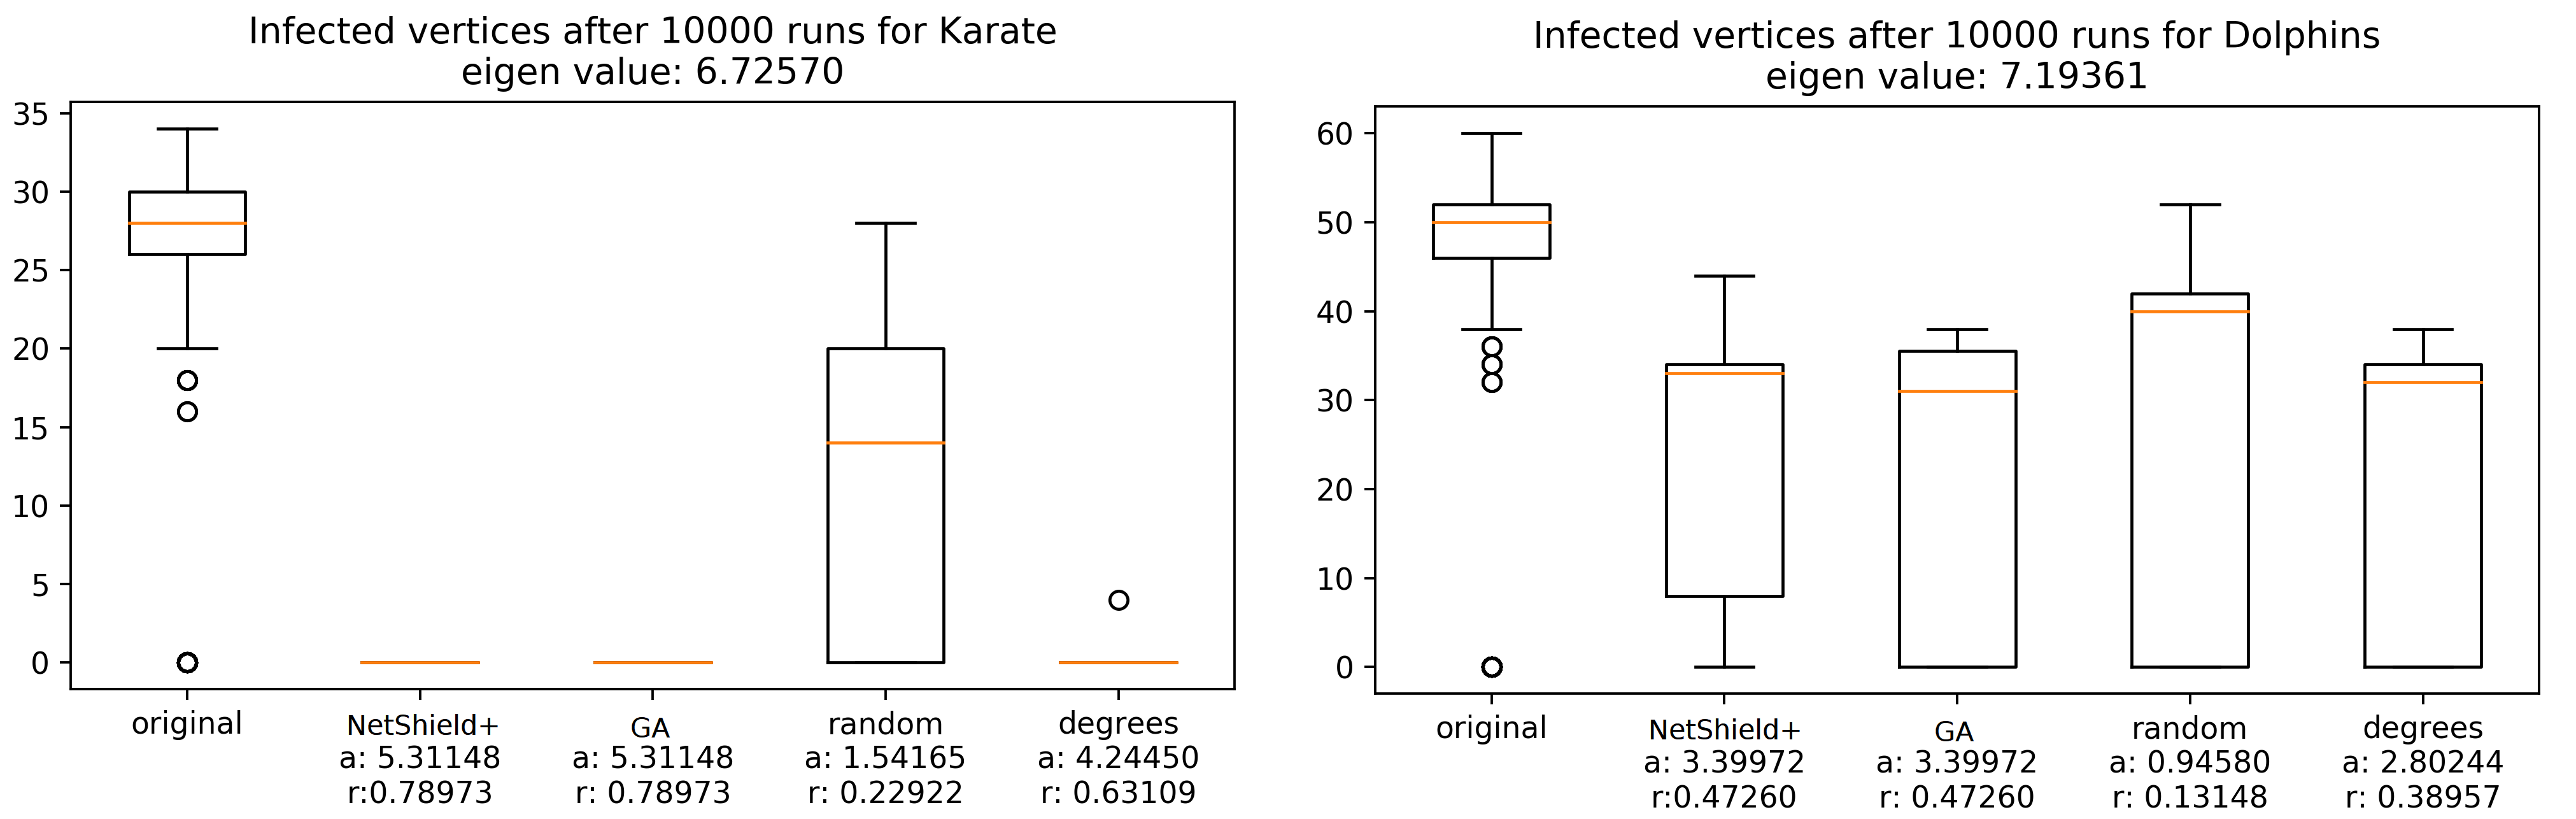
\includegraphics[width=1\textwidth]{sim_res_e/Karate_Dolphin}
  \caption{Simulation results for Karate and Dolphin graphs. 'a' denotes the absolute eigen-drop, 'r' denotes the percentage eigen-drop}
  \label{fig:sim_karate_dolphin}
\end{figure}

\begin{figure}[h!]
  \centering
    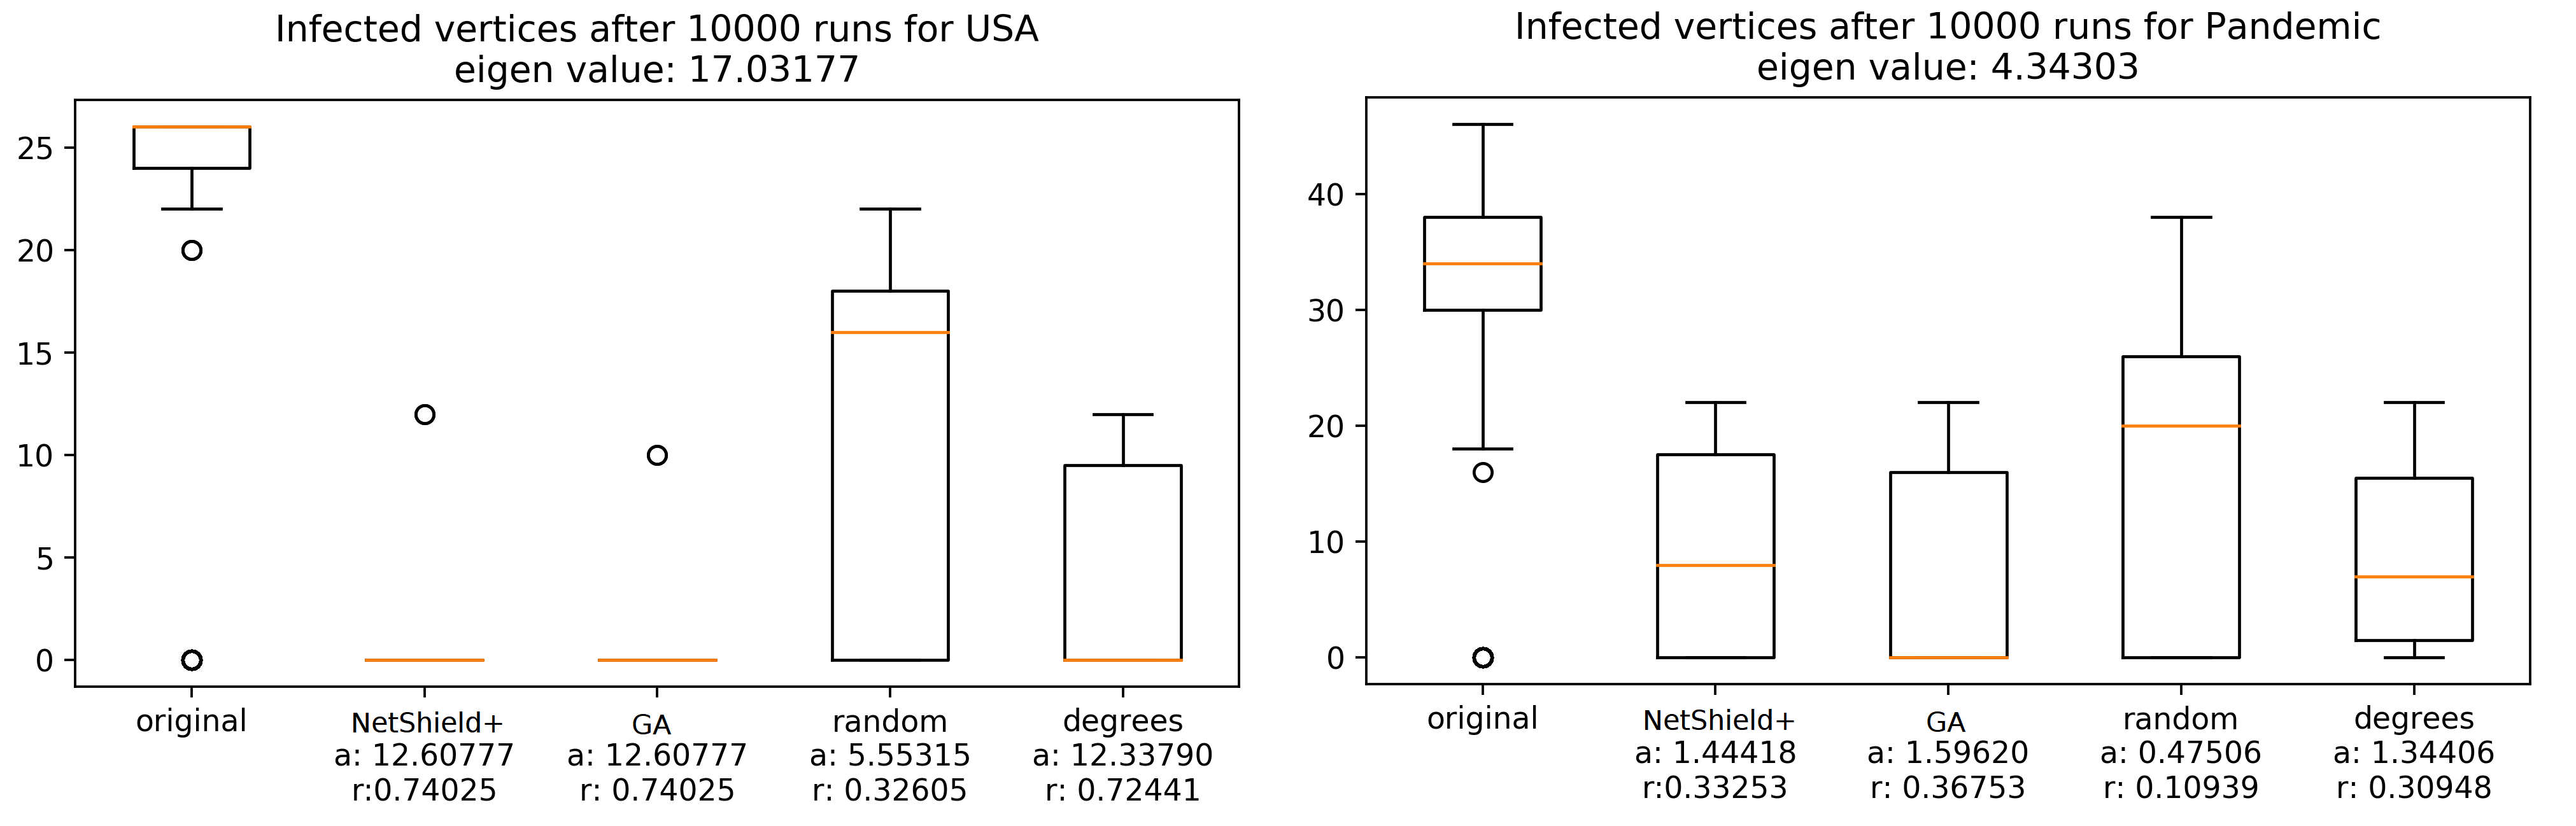
\includegraphics[width=1\textwidth]{sim_res_e/usa_pandemic}
  \caption{Simulation results for USA and Pandemic graphs. 'a' denotes the absolute eigen-drop, 'r' denotes the percentage eigen-drop}
  \label{fig:sim_usa_pandemic}
\end{figure}

\begin{figure}[h!]
  \centering
    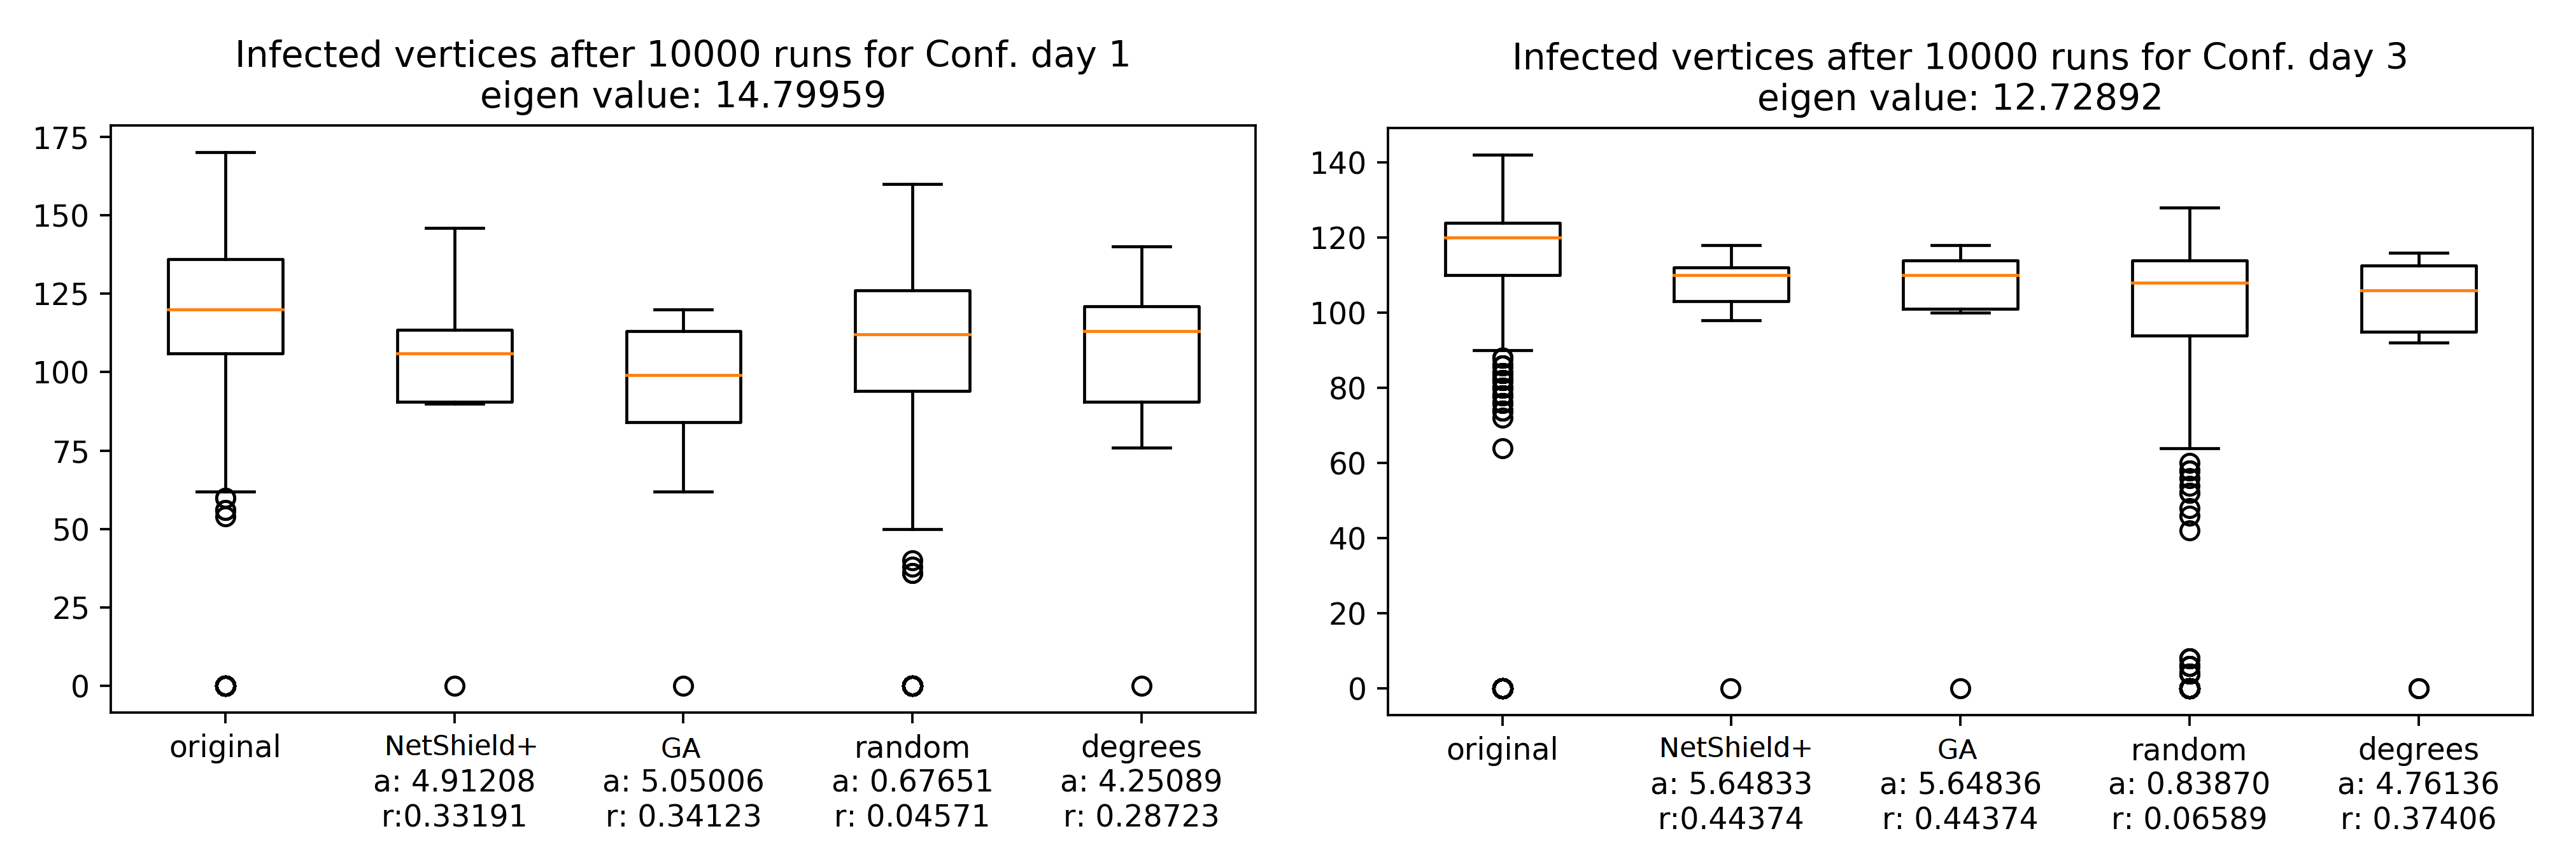
\includegraphics[width=1\textwidth]{sim_res_e/day1_day3}
  \caption{Simulation results for Conf. day 1 and Conf. day 3 graphs. 'a' denotes the absolute eigen-drop, 'r' denotes the percentage eigen-drop}
  \label{fig:sim_day1_day3}
\end{figure}

\begin{figure}[h!]
  \centering
    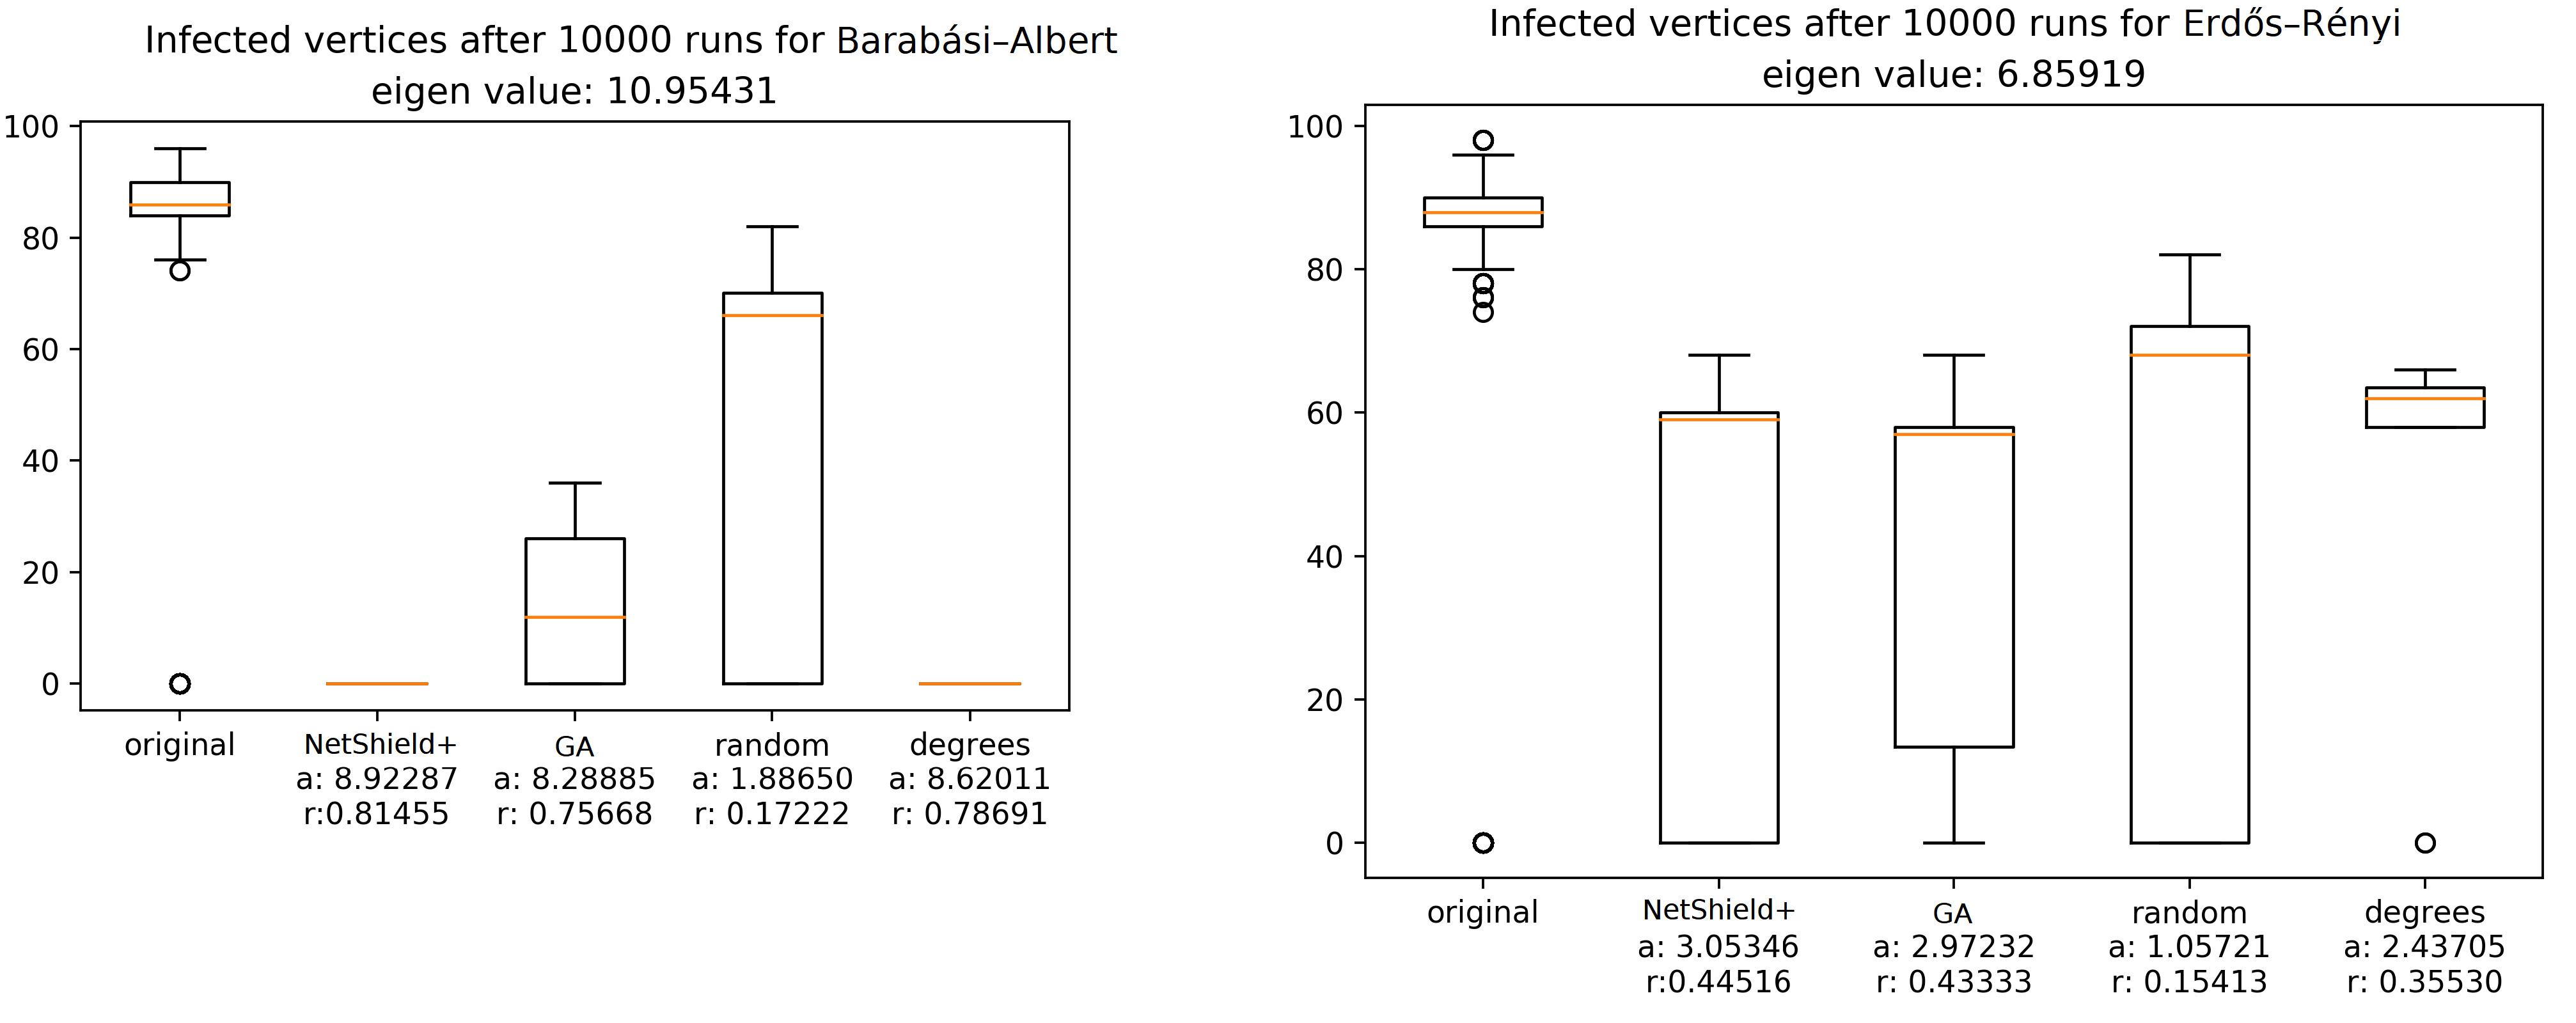
\includegraphics[width=1\textwidth]{sim_res_e/Barabasi_Erdos}
  \caption{Simulation results for Barab\'asi-Albert graph and Erd\H{o}s-R\'enyi graph. day 1 and Conf. day 3 graphs.'a' denotes the absolute eigen-drop, 'r' denotes the percentage eigen-drop}
  \label{fig:sim_barabasi_erdos}
\end{figure}



\cleardoublepage

\section{ Multi-Objective Node Immunisation }

For the $k$-node immunisation problem, every node is treated as having an equal cost. It is then the task to find the best possible solution that contains $k$ nodes. This may not always translate well to real world scenarios. For example, it may be that the nodes of a network represent cities to be immunised. In such scenarios it is likely that it is more expensive to immunise a large city than a small town, but more effective in terms of immunisation of the network. It appears then that there is a trade-off between two objectives: maximisation of the immunisation effect and minimisation of the total cost. Furthermore, the methods for the $k$-node problem, require that $k$ is known a priori. A good value of $k$ may however not been known a priori. By defining the immunisation problem as a multi-objective problem, the trade-off between eigen-drop and cost can be captured and no value of $k$ is needed:

\begin{equation}
\begin{gathered}
\Delta\lambda = \lambda - \lambda' \to \max \\
Cost = \sum_{i \in S} Cost(i) \to \min \\
\end{gathered}
\end{equation}

Here the effectiveness of the immunisation is again defined as the eigen-drop caused by removal of the nodes in the set $S$ from the network. The cost is defined as the sum of the cost of removal of each individual node in the solution set. Instead of a single solution that would maximise only the first objective, we are now looking for the Pareto front. This is the set of solutions that can no longer be improved in a single objective without worsening the other. Solutions that are not on the Pareto front are dominated by at least one other solution. The solutions that lie on the Pareto front form the efficient set. For this problem these are all the solutions for which no better immunisation can be achieved without raising the cost.

In this chapter we devise two ways to approximate the Pareto front for this problem. The first is combining the NetShield and NetShield+ algorithms with the $\epsilon$-constraint method. The second is using two different genetic algorithms specifically designed for multi-objective optimisation problems. For more about multi-objective optimisation and methods to solve such problems, we point the reader to~\cite{emmerich2018tutorial} and~\cite{KaisaNMO}.


\subsection{NetShield with $\epsilon$-constraint method}

For this method the Shield-value function is again used as an approximation method, instead of working directly on the eigen-drop. In combination with the cost function, the problem definition is as follows:

\begin{equation}
\begin{gathered}
\text{Given an adjacency matrix A, its first eigenvalue $\lambda$ and its first eigenvector $u$, the objectives read:}\\
f_{1}(x) = \sum_{i=1}^{m} 2 \lambda  u_{i}^{2} x_{i} - \sum_{i=1}^{m} \sum_{j=i+1}^{m} u_{i} u_{j} A_{ij}  x_{i} x_{j} \to \max \\
f_{2}(x) = \sum_{i=1}^{m} x_{i} * Cost(i) \to \min\\
\text{Subject to:}\\
x \in \{0,1\}^{m}
\end{gathered}
\end{equation}

Here the solution is again represented as a binary vector. The first objective function is to maximise the eigenvalue drop, whereas the second objective function is to minimise the cost.

The $\epsilon$ constraint method works by transforming one of the objectives in a constraint~\cite{KaisaNMO}. For the NetShield program, we have chosen this to be the cost function. 

\begin{equation}
\begin{gathered}
\text{Given an adjacency matrix A, its first eigenvalue $\lambda$ and its first eigenvector $u$:}\\
f_{1}(x) = \sum_{i=1}^{m} 2 \lambda  u_{i}^{2} x_{i} - \sum_{i=1}^{m} \sum_{j=i+1}^{m} u_{i} u_{j} A_{ij} x_{i} x_{j} \to \max \\
\text{Subject to:}\\
f_{2}(x) = \sum_{i=1}^{m} x_{i} * Cost(i) \leq \epsilon\\
x \in \{0,1\}^{m}
\end{gathered}
\end{equation}

Then by solving this problem multiple time with different values for $\epsilon$, it is possible to sample multiple points that lie on the Pareto front of the cost and Shield-value objectives. As the Shield-value can be a good approximation of the actual eigen-drop, this should then translate in a good approximation of the Pareto front of the eigen-drop and cost objectives. The transformed problems are examples of quadratic integer problems with a linear constraint. Therefore we can again optimise these via a quadratic program solver.

To deal with the inaccuracy of the Shield-value function in case a larger number of nodes is removed, this method can be extended similarly to the way it is done for the NetShield+ algorithm. This is done by adding an extra constraint that limits the number of vertices to the same batch size as used in the NetShield+ algorithm. This limits the number of vertices that can be added to the solution during the optimisation. After an intermediate solution is found, the found nodes can be removed from the matrix and added to the complete solution set. Then a new Shield-value function can be created with the new first eigenvalue and eigenvector. This process can be repeated until no more nodes can be added. This happens when all nodes are already added to the solution or because no new nodes can be added without violating the $\epsilon$-constraint. This procedure is also described in Algorithm \ref{alg:enetshieldp}

The extra constraints added are still linear constraints, meaning that all programs are still quadratic linearly constrained ones. Just as with the NetShield+ algorithm, if the batch size is set to 1, the second part of the Shield-value function will always be 0. This means that the programs in this case change to integer linear programs. While in general solving an integer linear program is still NP-complete, the very restricted search space makes these special instances straightforward to solve.

\begin{algorithm}
  \caption{NetShield+ with $\epsilon$-constraint
    \label{alg:enetshieldp}}
  \begin{algorithmic}[1]
    \Require{An adjacency matrix $A$, batch size $b$ and constraint $\epsilon$ and cost function}
    
    \Statex
    \Let{$s$}{ $(0,..,0) \in {0,1}^m $}
    \Let{done\_flag}{false}
    \While{done\_flag is false}
        \Let{$\lambda, u$}{Compute from A}
       \begin{equation}
            \begin{gathered}
            \text{Solve:}\\
            \sum_{i=1}^{m} 2 \lambda  u_{i}^{2} x_{i} - \sum_{i=1}^{m} \sum_{j=i+1}^{m} u_{i} u_{j} A_{ij} x_{i} x_{j}\to \max \\
            \text{Subject to:}\\
            \sum_{i=1}^{m} x_{i} \cdot Cost(i) \leq \epsilon\\
            \sum_{i=1}^{m} x_{i} \leq \sum_{i=1}^m s_i + b \\
            \sum_{i=1}^{m} x_{i} > \sum_{i=1}^m s_i \\
            s_{i} = 1 \rightarrow x_{1} = 1 \\
            x \in \{0,1\}^{m} \\
            \end{gathered}
        \end{equation}
        
        \If{infeasible}
            \Let{done\_flag}{true}
        \Else
            \State Set $s_i$ to 1 where $x_i$ is 1.
            \State Remove node $i$ from $A$ for where $x_i$ is 1.
        \EndIf
    \EndWhile
  \end{algorithmic}
\end{algorithm}



\subsection{Multi-Objective Genetic Algorithms}

Several genetic algorithms have been designed for optimising multi-objective problems. The selection of solutions that survive to the next generation is straightforward if there is only a single fitness value. However, care must be taken in multi-objective problems. It is important that solutions do not cluster around a few points on the Pareto front, but that a good spread of solutions over the whole Pareto front is found. Two of these methods are described here. These will will also be used to approximate the Pareto fronts for the multi-objective node immunisation problem. They are NSGA-II ~\cite{deb2002fast} and SMS-EMOA ~\cite{emmerich2005emo}. Key to their design is the selection operator that aims to achieve convergence and spread.

First both algorithm partition the solutions into layers based on their dominance rank. Within these layers, no solutions dominate another, but all solutions in a lower ranked layer are dominated by at least one solution in the next higher ranked layer. Solutions in lower ranked layers are considered first for removal from the population.

Within the layers, both methods rank the solutions as well. The lowest ranked solution within in the lowest ranked layer will then be removed first. The methods differs in how they perform this ranking. The NSGA-II algorithm makes use of the crowding distance metric. This metric measures how close the solutions is to other solutions in the objective space. Solutions closely clustered together are given a lower rank than solutions that are further apart. See Figure \ref{fig:cde} for an example of the crowding distance of two points in a population in a 2D objective space.

\begin{figure}[h!]
  \centering
    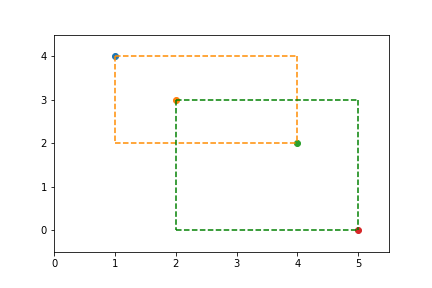
\includegraphics[width=0.75\textwidth]{other_img/crowding}
  \caption{Crowding Distance example of middle two points in 2-D. Crowding distance for each point is the circumference of the area denoted by the dotted lines}
  \label{fig:cde}
\end{figure}

The SMS-EMOA algorithm ranks within the group by using the hypervolume contribution which is defined for a population of mutually non-dominated solutions in the objective space. The hypervolume indicator (Lebesgue measure) is the size of the dominated hyperspace bound from above by a reference point. This point should be dominated by all possible solutions. Then each solution is ranked based on how much it contributes to the hypervolume indicator. Solutions that contribute more are ranked higher. As we are looking at a problem with two objectives, the objective space is two-dimensional and the hypervolume indicator will be the area of the dominated space truncated by the reference point. See Figure \ref{fig:chve} for an example.

\begin{figure}[h!]
  \centering
    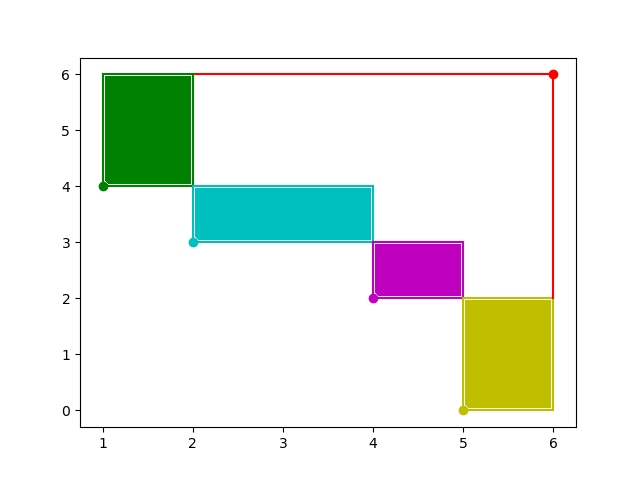
\includegraphics[width=0.75\textwidth]{other_img/hpc_example_filled}
  \caption{Example of 2-D hypervolume indicator (size of entire coloured region) and 2-D hypervolume contributions of points (size of coloured rectangular regions adjacent to the points). Both objectives are to be minimised and the reference point is located at (6,6)}
  \label{fig:chve}
\end{figure}

The rest of the genetic algorithms work similar to a traditional one. As we are now interested in solutions without a specific number of nodes, the representation used for the $k$-objective immunisation and consequently the mutation and crossover operators is no longer suitable. Instead the solutions are represented in a traditional manner: a binary vector of size equal to the number of nodes in the network. During mutation there is probability of $1/n$ for every bit to flip as proposed by \cite{BackBook}. The crossover method is 1-point crossover. For parent selection, two random solutions are chosen from the population. A $\mu+1$ selection scheme is used, meaning that every generation a single new solution is created and the worst of all solutions is removed from the population.


\subsection{Hybrid Approach}

Using the NetShield or NetShield+ $\epsilon$-constraint method, a good approximation of the Pareto front may be found. By using the solutions from these methods as the initial population of the SMS-EMOA and NSGA-II GAs described above, it may be possible to further refine the solution set. This cuts out the potentially large search effort needed to come to a good Pareto front approximation by the GAs on their own. Then their ability to directly work on the actual objective-function instead of an approximation may explore solutions around the initial population that were not considered by the NetShield-algorithms that would further improve the solution set.

\subsection{Experiments and Results}

The data set used for the experiments is the same one as for the experiments in section 4. Furthermore, it is necessary to define a specific cost function. This cost function should be a good measure for the effort required for the removal of a node. For example the population size of cities could be used for the Pandemic board game graph or the number of flights could be chosen for the airports in the USA graph. Our data set however, also contains graphs that do not represent any real world network, but are instead sampled from two random graph models. Therefore, we made the choice to take the degree of a node as its immunisation cost. To keep the results comparable between graphs, we kept this cost function for all graphs. As section 3 showed a strong correlation between average degree and eigenvalue, nodes with a larger degree should in general be more important to the immunisation. This would make it so that the cost of each node would be roughly equivalent to the impact on immunisation, making it a suitable substitute for an actual real world cost function.

All of the GAs were run 5 times under each configuration, both when the population was initialised at random and when initialised with the NetShield solutions. The populations were set at a size of 100 for the random initialisation. The mutation probability $p_m$ was set to $1/n$, with $n$ being the number of vertices of the graph. Crossover probability $p_c$ was set to $0.75$. The reference-point for the SMS-EMOA algorithm was set to an eigen-drop value of -1 and cost was set to the the sum of all degrees plus 1. As the eigen-drop will always be positive when only removing nodes from a network and the cost of any possible solution will at most be the sum of all degrees, this ensures that every possible solution will dominate the reference point. All GAs were run for 10000 iterations.

Both the NetShield and NetShield+ methods with the $\epsilon$-constraint method were tested. For the NetShield+ method, the batch size was set to 1. The resolution of the Pareto front approximation depends on how many different values of $\epsilon$ are sampled. As the cost function chosen uses only non-negative integers, it is possible to get the best possible resolution by sampling only a finite amount of points: from 0 to the sum of all degrees increasing $\epsilon$ by 1 every step.

\subsubsection{NetShield with $\epsilon$-constraints and GAs}

The results of both the NetShield methods and the GAs are plotted in Figure~\ref{fig:karate_atns} to~\ref{fig:baral_atns}. For the GAs the first attainment curve is plotted. The $j$-th attainment curve is a set of points that are weakly dominated by $j$ runs out of the total number of runs \cite{Fonseca96a} \cite{Fonseca01}. Therefore these first attainment curves represent best case scenarios for the GAs.

When comparing the NSGA-II algorithm to the SMS-EMOA algorithm, no clear differences show. It changes from graph to graph which algorithm finds the better Pareto front approximation and the results consistently lie very closely together.

Differences do show when comparing the performance of the NetShield method with the NetShield+ method. Sometimes the differences are minor, e.g. the USA graph in Figure \ref{fig:USA_atns}. For other graphs the difference can be more significant, e.g. Figures \ref{fig:dolphin_atns}, \ref{fig:Pandemic_atns}, \ref{fig:day1_atns} and \ref{fig:day3_atns}. This is most likely due to the Shield-Value losing accuracy when the number of nodes removed increases. This shows in the figures: Initially the performance of NetShield is very similar to NetShield+. When the allowed cost increases and consequently more nodes can be selected, the NetShield+ method can find solutions that are significantly better. 

At the rightmost extremes however, the NetShield method sometimes finds a few better solutions that dominate those found by the NetShield+ method. See for example the  Erd\H{o}s-R\'enyi graph in figure \ref{fig:erdos_renyi_atns}, the Dolphins graph in Figure \ref{fig:dolphin_atns} and the Barab\'asi-Albert graph in \ref{fig:baral_atns}. In addition at the bottom left of the Conference day 3 graph in figure \ref{fig:day3_atns} there are gaps in the Pareto front found by the NetShield+ method where the NetShield method does find solutions. This may be because the NetShield+ method with a batch size of 1 is more greedy than the NetShield method. With a batch size of 1, the NetShield+ method selects at every step the node with the highest eigen-score that would not violate the $\epsilon$-constraint when added to the solution. It then recomputes a new Shield-value function with the node removed. The NetShield method however, only computes the Shield-value function at the beginning and selects multiple nodes at once to optimise this function. In this way it can take a more global view of the problem and if the Shield-Value happens to be a good approximation of the eigen-drop, better solution may be found. A possible approach would therefore be to repeat the NetShield+ method several times with different batch sizes if time allows. Then all results can be combined for the most accurate Pareto front approximation by filtering out all solutions dominated by another.

When comparing both the NetShield methods with the GAs, the GAs give very competitive performance for the smaller graphs. Here the search space is relatively small and the GAs have enough time to converge on the Pareto front. This results in some parts of the Pareto front being approximated better by the GAs, because they can work directly on the eigen-drop. See for example the karate graph in \ref{fig:karate_atns} and pandemic graph in figure \ref{fig:Pandemic_atns}. For the pandemic graph in particular, both NetShield methods have problems converging on the Pareto front. Just as in chapter 4, this is likely caused by this graph having a low maximum degree. This means that the Shield-value approximation loses accuracy quickly. However, the NetShield algorithms do appear to be better at finding points in the rightmost extremes than the GAs. 

When the search space is too large, however, it appears that the GAs lose effectiveness. This is shown in the results for the largest graphs: Conference day 1 and Conference day 3 in Figures \ref{fig:day1_atns} and \ref{fig:day3_atns}. Here the GAs do appear to be in the process of nearing the results of the NetShield+ method. They may give better approximations when the number of iterations is increased further, but the NetShield+ method outperforms them significantly under the used configuration.

When looking at the shape of the Pareto fronts, they can roughly be grouped in three different categories. The first are those whose Pareto fronts are roughly linear. These are the Karate graph in \ref{fig:karate}, the dolphins graph in Figure \ref{fig:dolphin_atns}, the pandemic graph in Figure  \ref{fig:Pandemic_atns} and the Erd\H{o}s-R\'enyi graph in Figure \ref{fig:erdos_renyi_atns}. Here the cost measure of the degree appears to strongly correlate with the eigen-drop. For the Erd\H{o}s-R\'enyi graph however, the two points found at the rightmost extreme by the NetShield method show a big increase in eigen-drop combined with a relatively low cost increase. Here the value chosen for $\epsilon$ allows for a large drop in eigen-value by making the graph fall apart with larger set of nodes with lower costs. As a result the Pareto front for this graph has a concave section at the end. 

The second group contains both the Conference graphs in Figure \ref{fig:day1_atns} and \ref{fig:day3_atns}. These Pareto fronts show the strongest bend in the middle. Initially, the eigen-drop increases quickly when compared to the cost. Eventually diminishing returns set in: higher costs are needed to get the same improvements in eigen-drop. 

The last category is the Barab\'asi-Albert graph in Figure \ref{fig:baral_atns}. This Figure shows that the Pareto front consists of several parts that are mostly linear, but also that there are a some gaps between these linear sections.  At these gaps the eigen-drop suddenly increases significantly with only a small increase in cost. The solution sets at the three biggest gaps are visualised in Figures \ref{fig:j1}, \ref{fig:j2} and \ref{fig:j3}.  The nodes in these visualisations are scaled by degree. The Figures show that at these points the cost budgets are increased enough so that a new high cost node can be added to the solution set, replacing a set of lower cost nodes. These high cost nodes are the ones that due to the preferential attachment mechanism of the Barab\'asi-Albert model have become the hubs of the network. Despite their large cost however, the impact of these nodes on the eigen-drop is still disproportionate, which causes the gaps in the Pareto front. 

In conclusion, which method works best depends in terms of quality of the Pareto front approximation depends on the size of the search space, in this case the number of vertices of the graph, and how accurate the Shield-value metric is for a graph. In case the search space is relatively constrained or the Shield-value is not accurate, the GAs give the better results. Otherwise, the NetShield(+) based methods have the advantage. No individual method gives the best results in all cases. In addition, the GAs also require a longer run time. The results also show that there appears to be no typical shape for the Pareto fronts for this problem. They depend on how the cost measure is chosen and how it correlates to the importance of the nodes in the network.


\begin{figure}[h!]
  \centering
    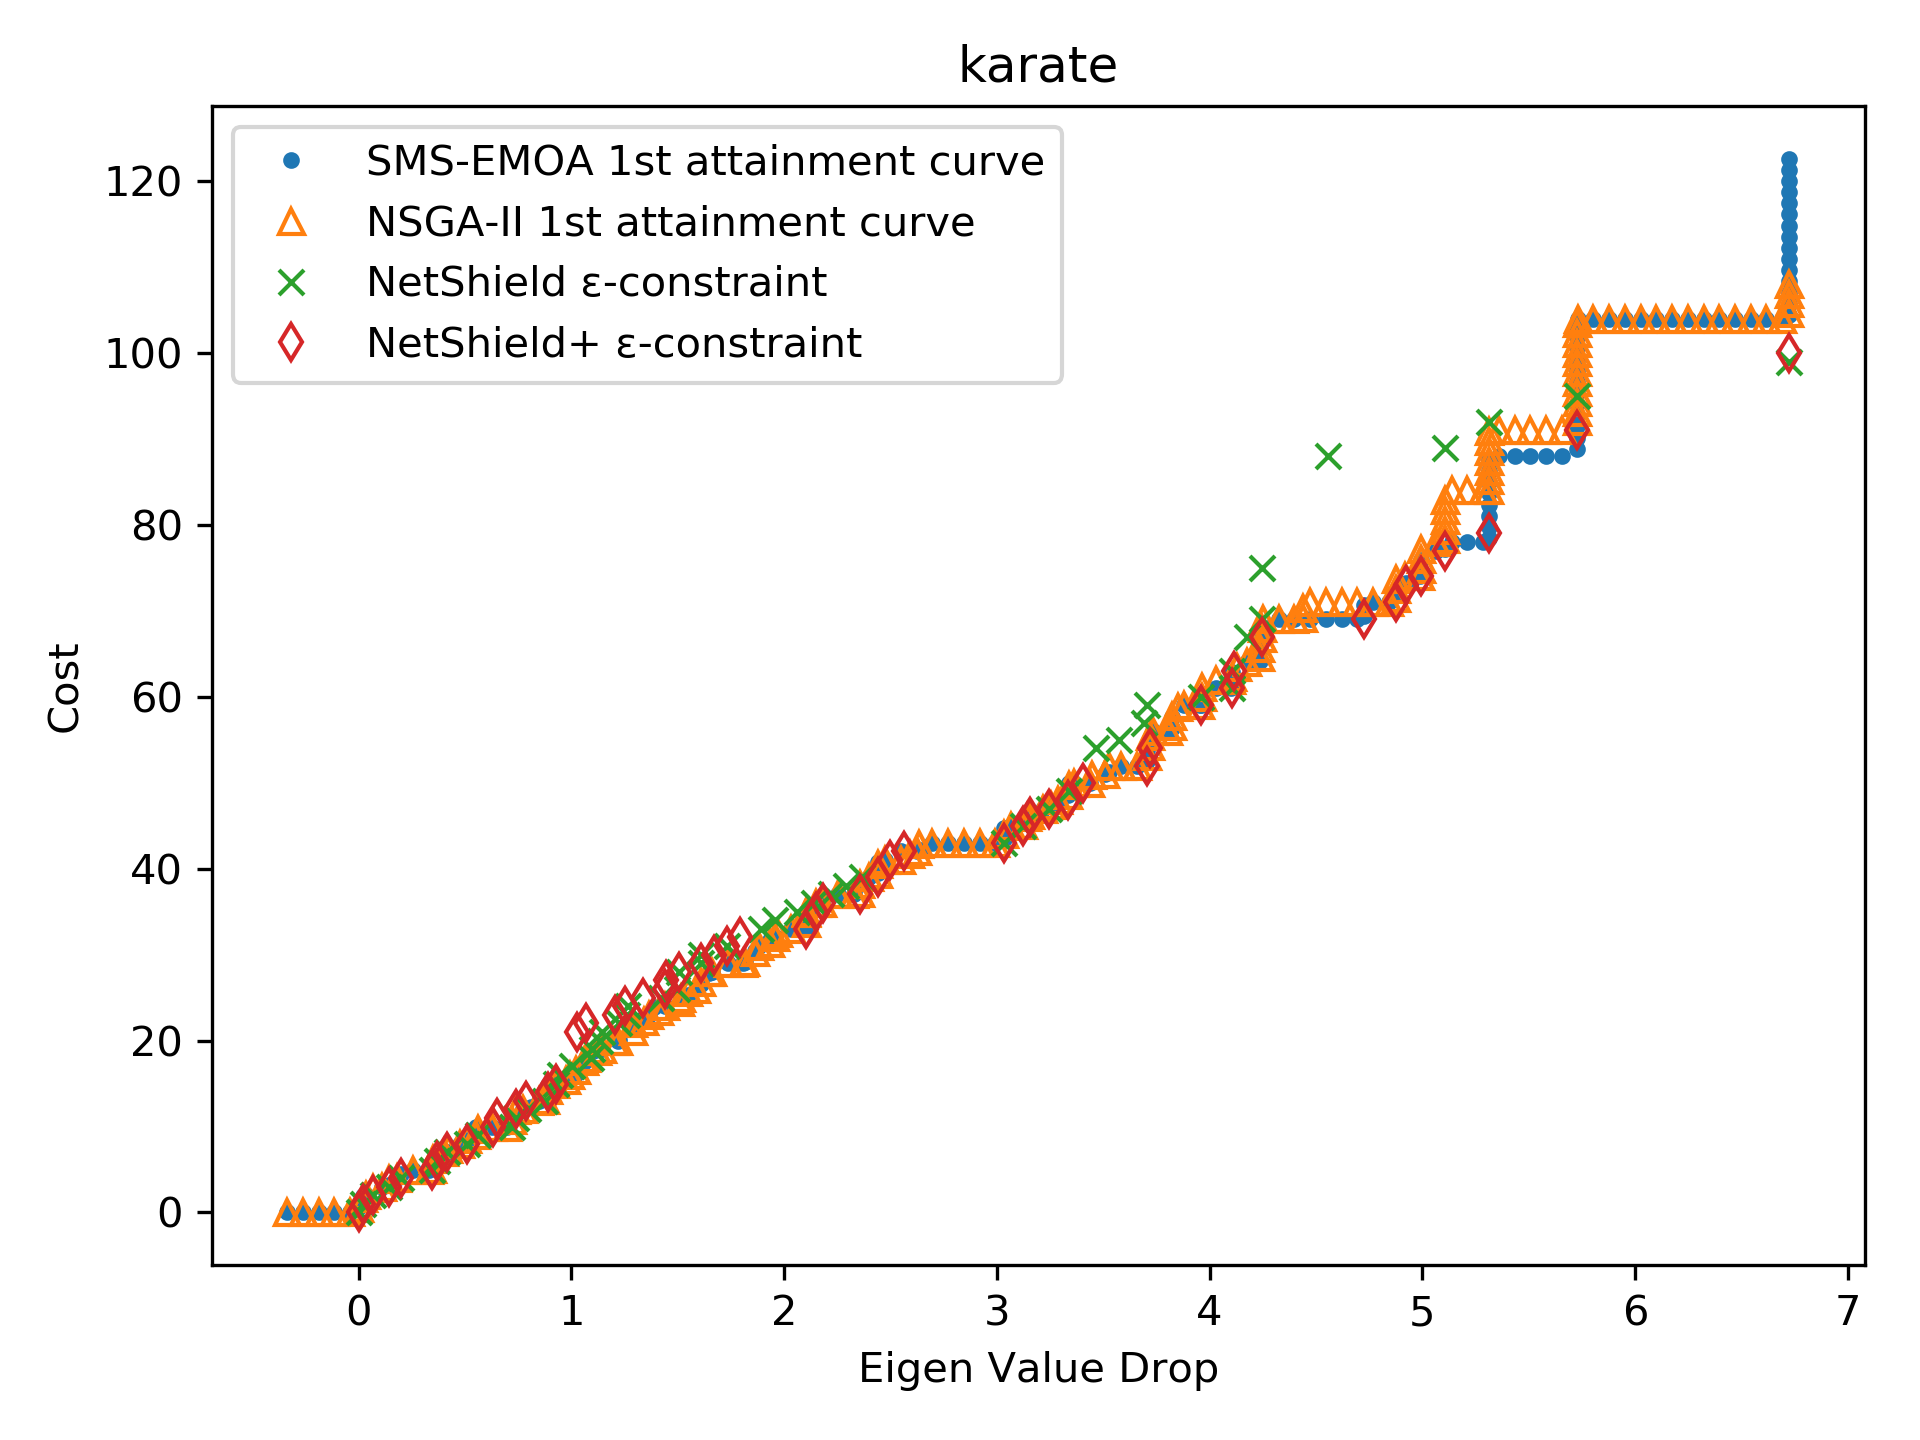
\includegraphics[width=0.75\textwidth]{results_ns_ga/karate_attaintment_netshield}
  \caption{Pareto front approximations of the GAs and NetShield(+) with $\epsilon$-constraint methods for the karate graph}
  \label{fig:karate_atns}
\end{figure}

\begin{figure}[h!]
  \centering
    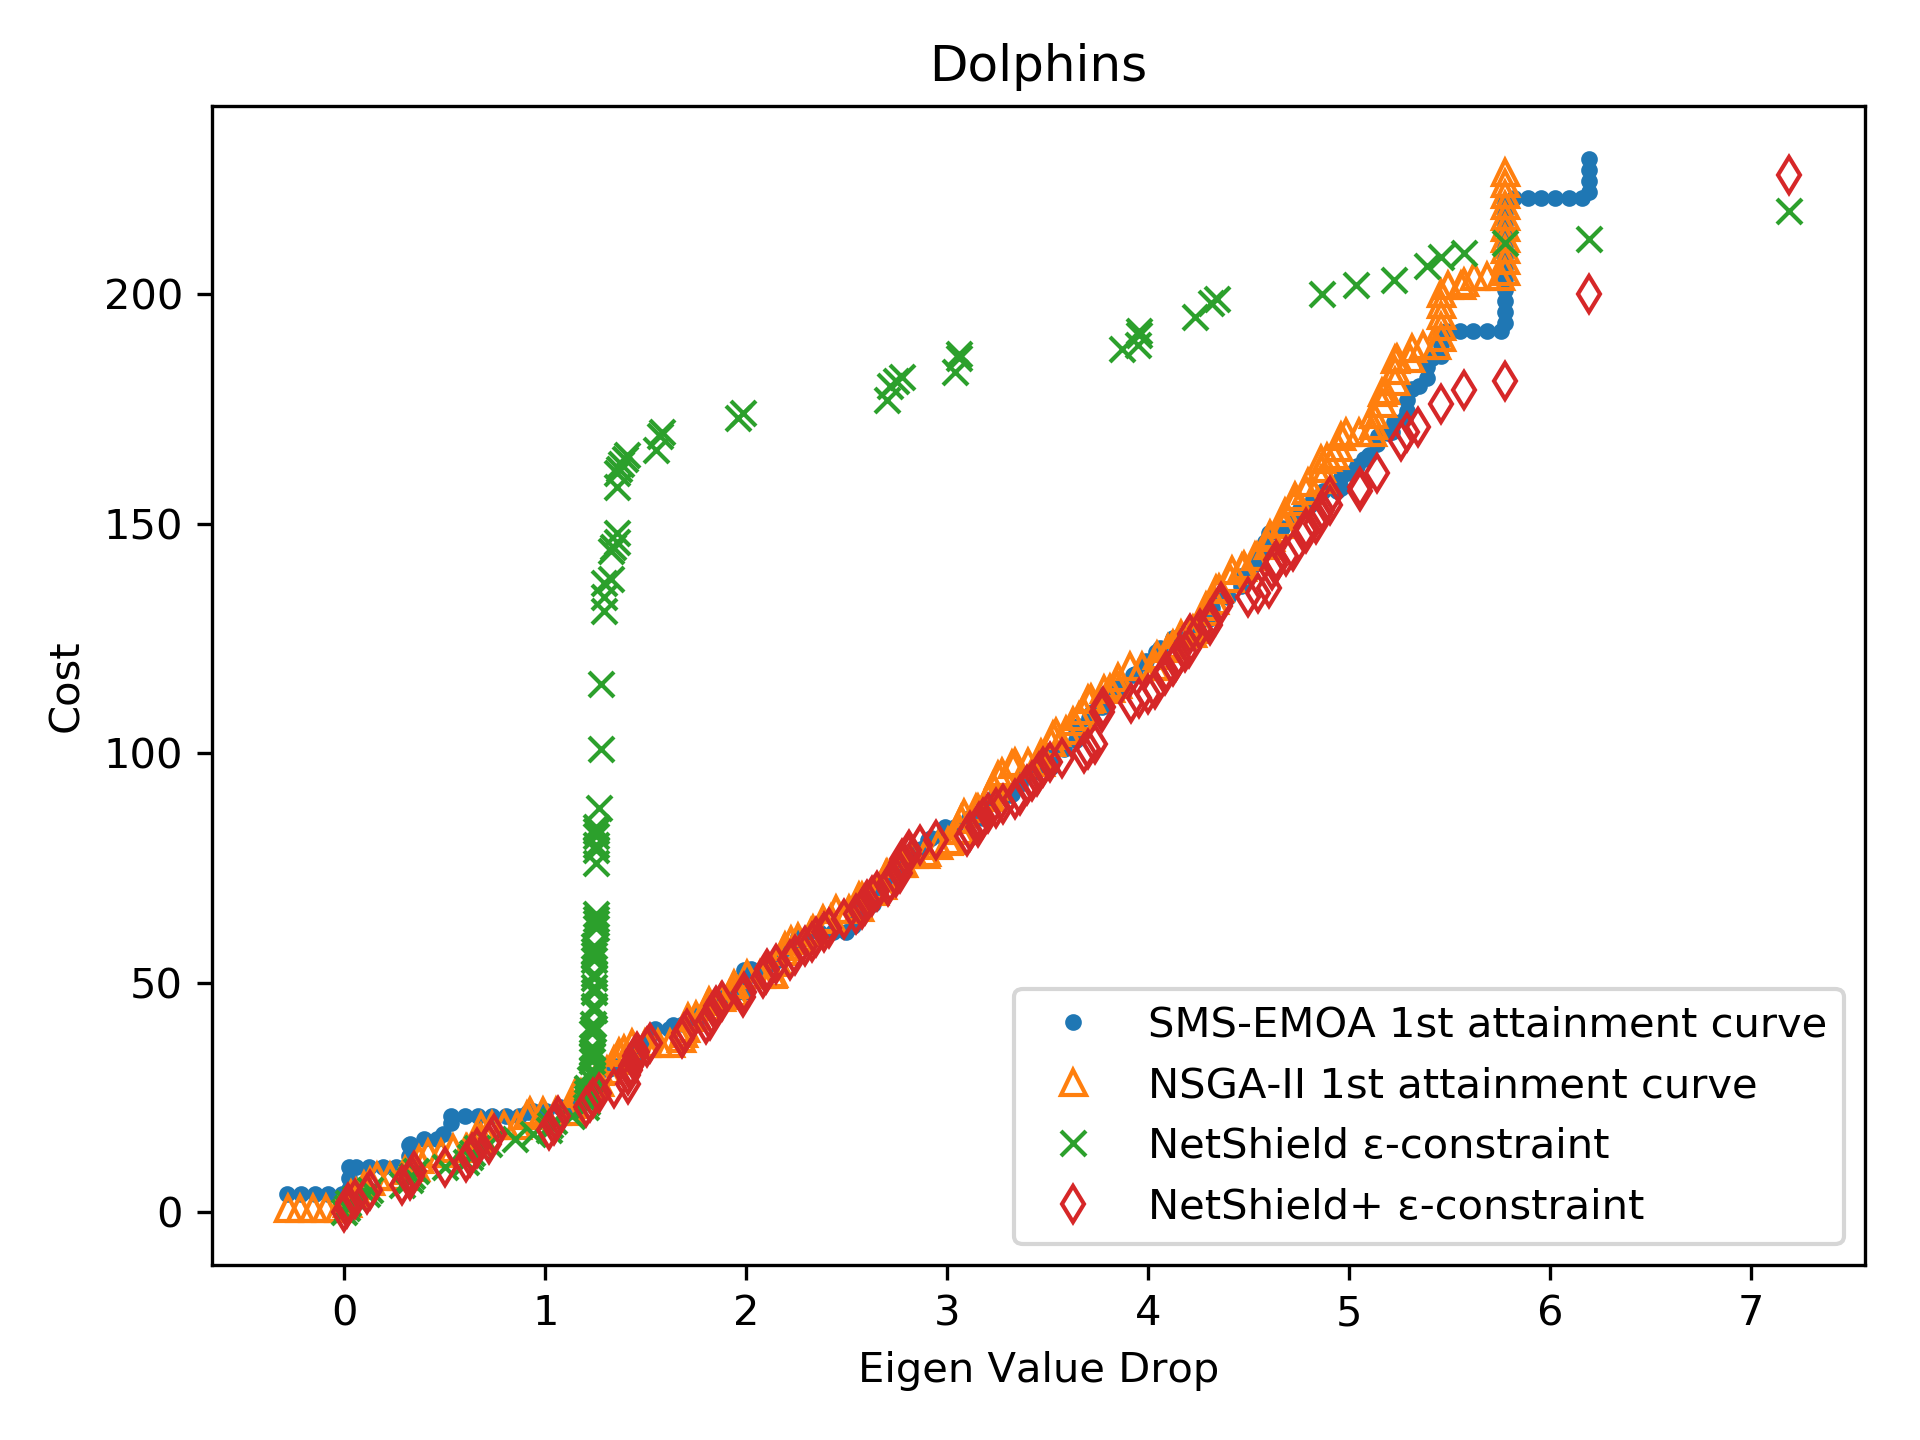
\includegraphics[width=0.75\textwidth]{results_ns_ga/dolphins_attaintment_netshield}
  \caption{Pareto front approximations of the GAs and NetShield(+) with $\epsilon$-constraint methods for the Dolphins graph}
  \label{fig:dolphin_atns}
\end{figure}

\begin{figure}[h!]
  \centering
    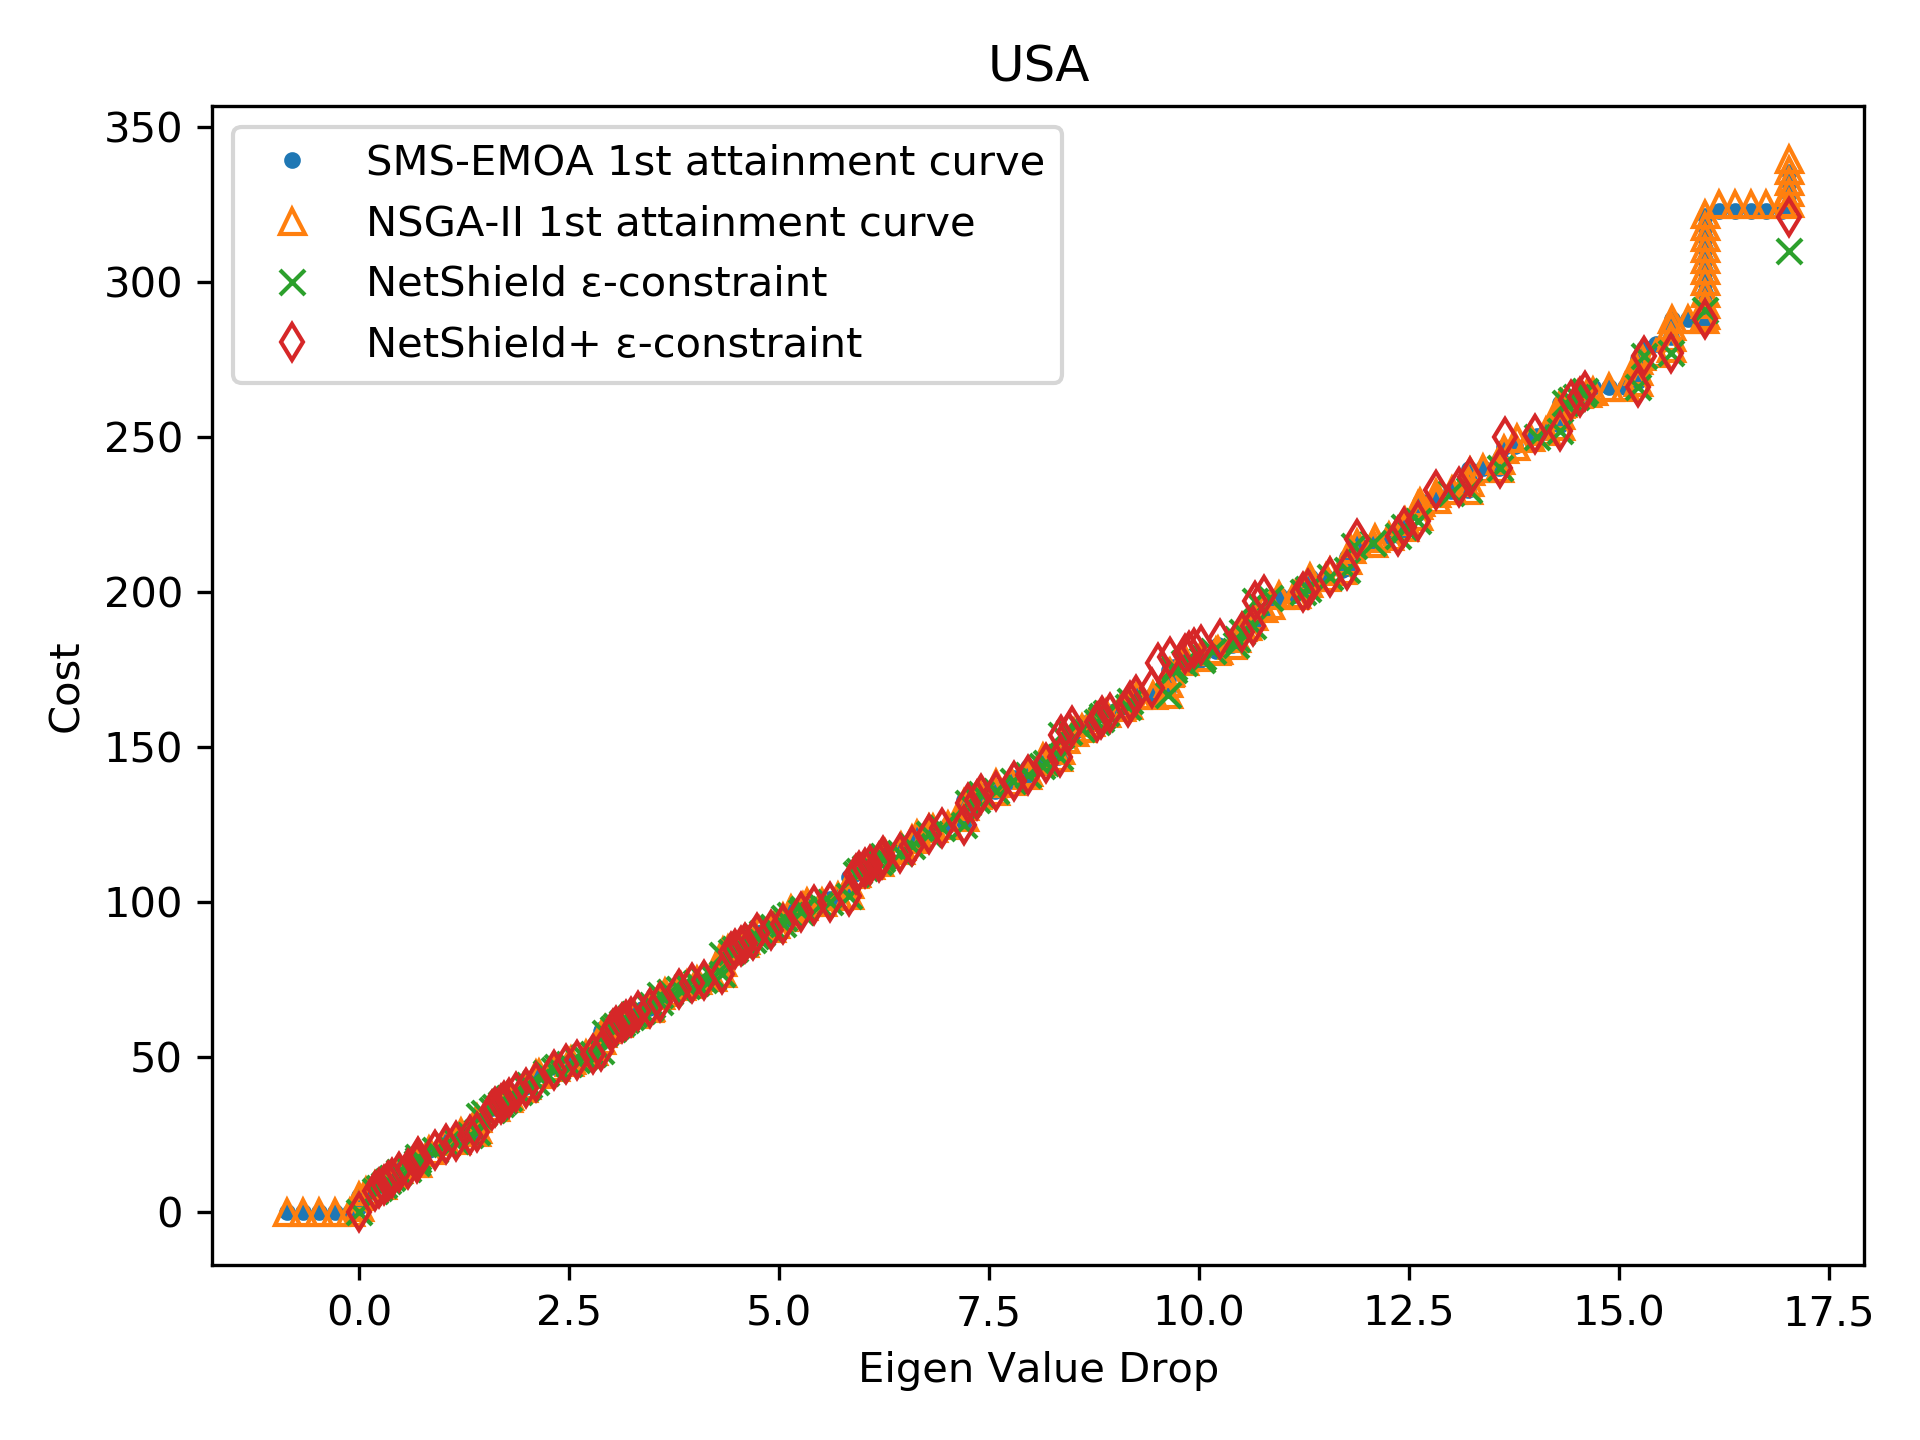
\includegraphics[width=0.75\textwidth]{results_ns_ga/USA_attaintment_netshield}
  \caption{Pareto front approximations of the GAs and NetShield(+) with $\epsilon$-constraint methods for the USA graph}
  \label{fig:USA_atns}
\end{figure}

\begin{figure}[h!]
  \centering
    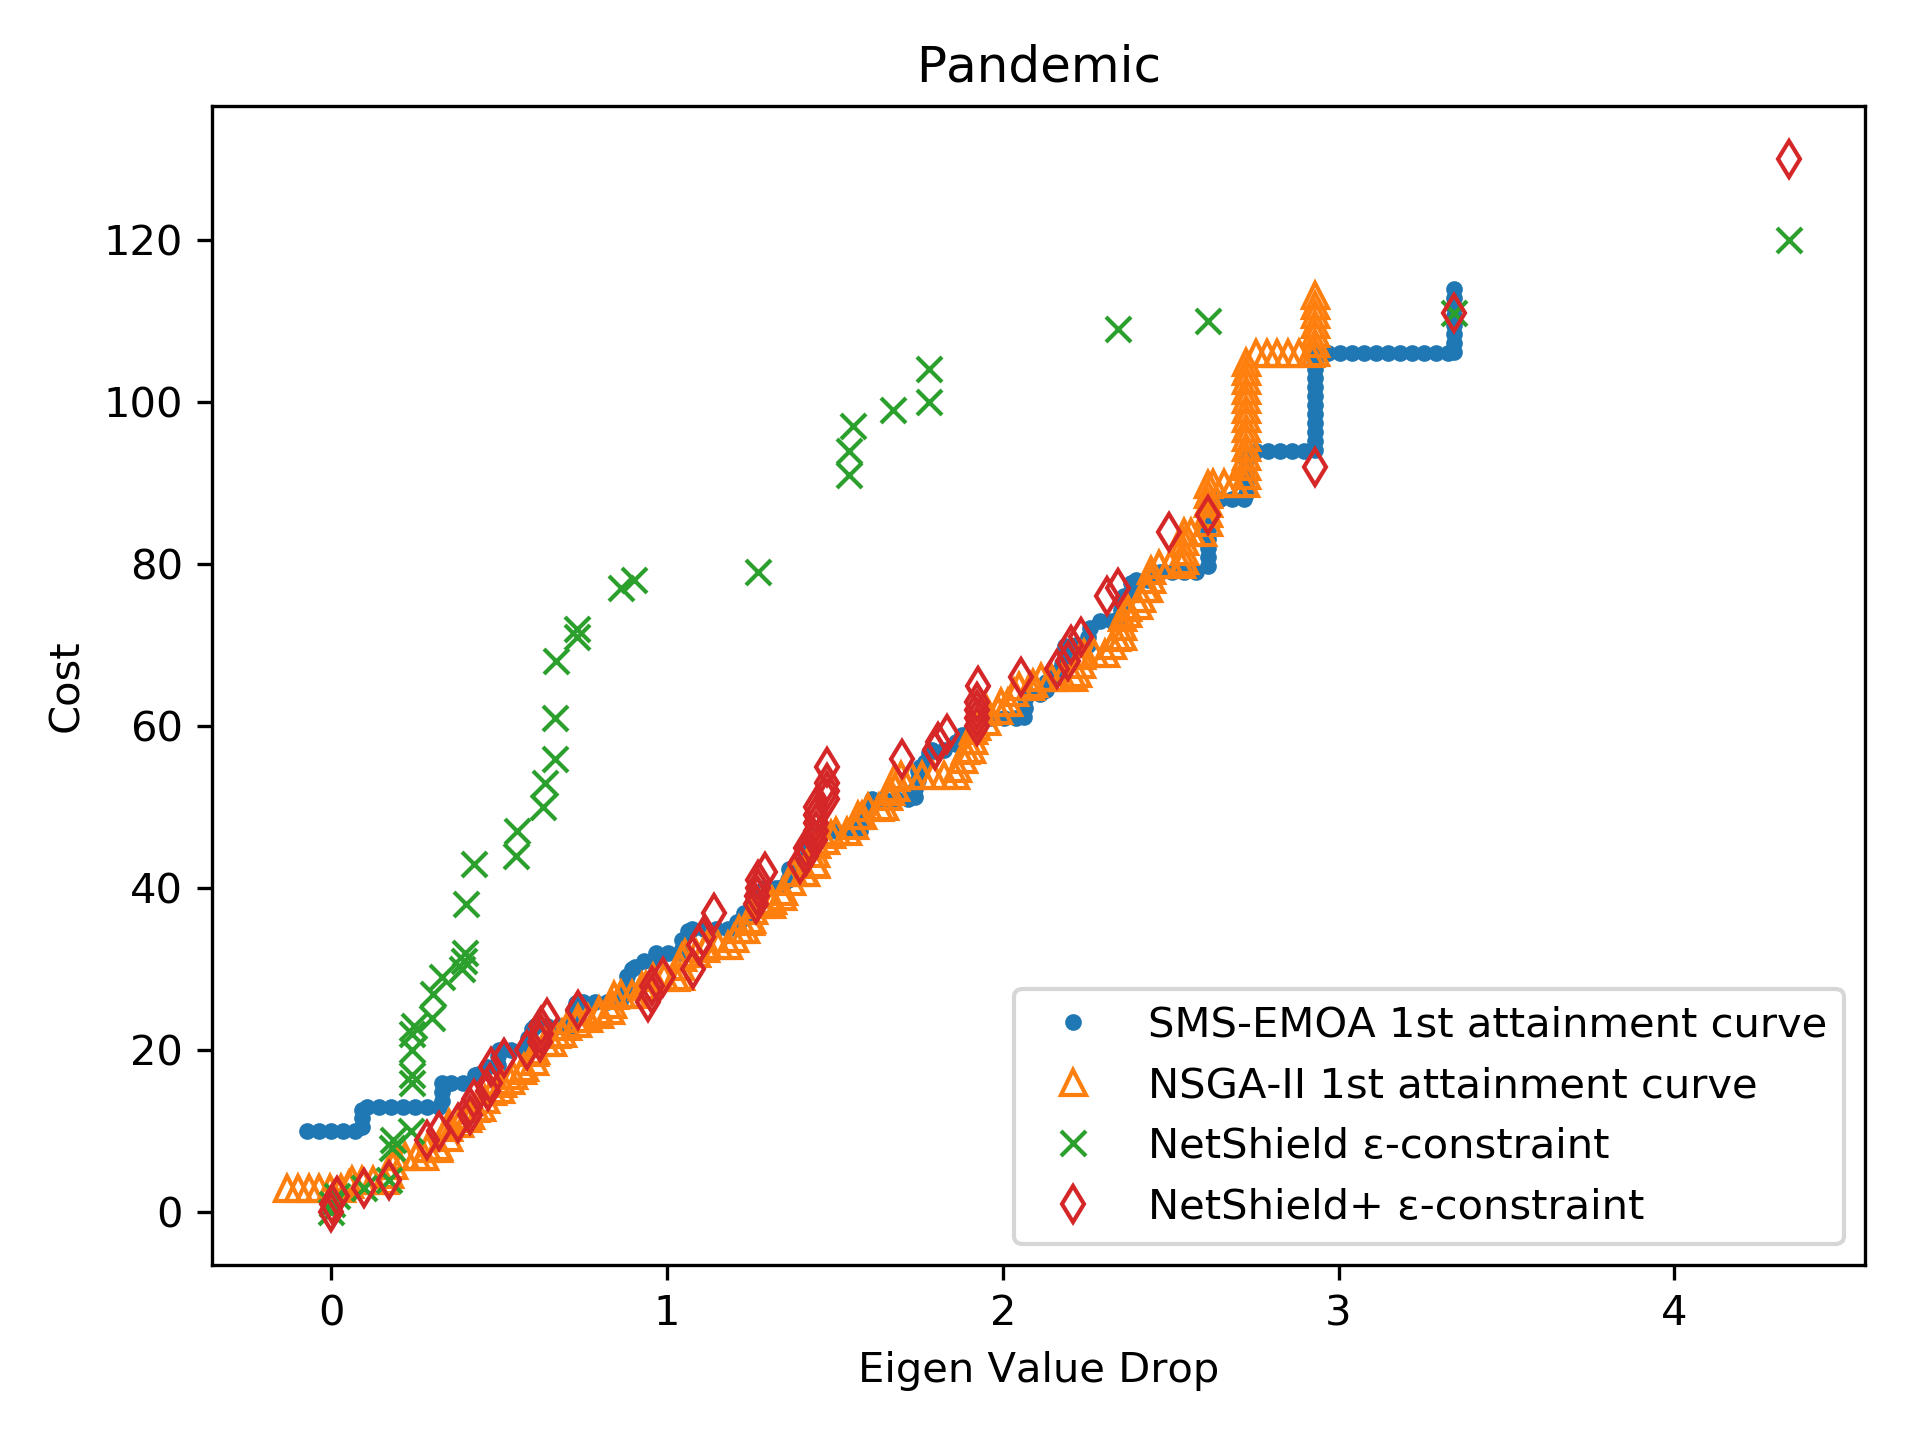
\includegraphics[width=0.75\textwidth]{results_ns_ga/pandemic_attaintment_netshield}
  \caption{Pareto front approximations of the GAs and NetShield(+) with $\epsilon$-constraint methods for the Pandemic graph}
  \label{fig:Pandemic_atns}
\end{figure}

\begin{figure}[h!]
  \centering
    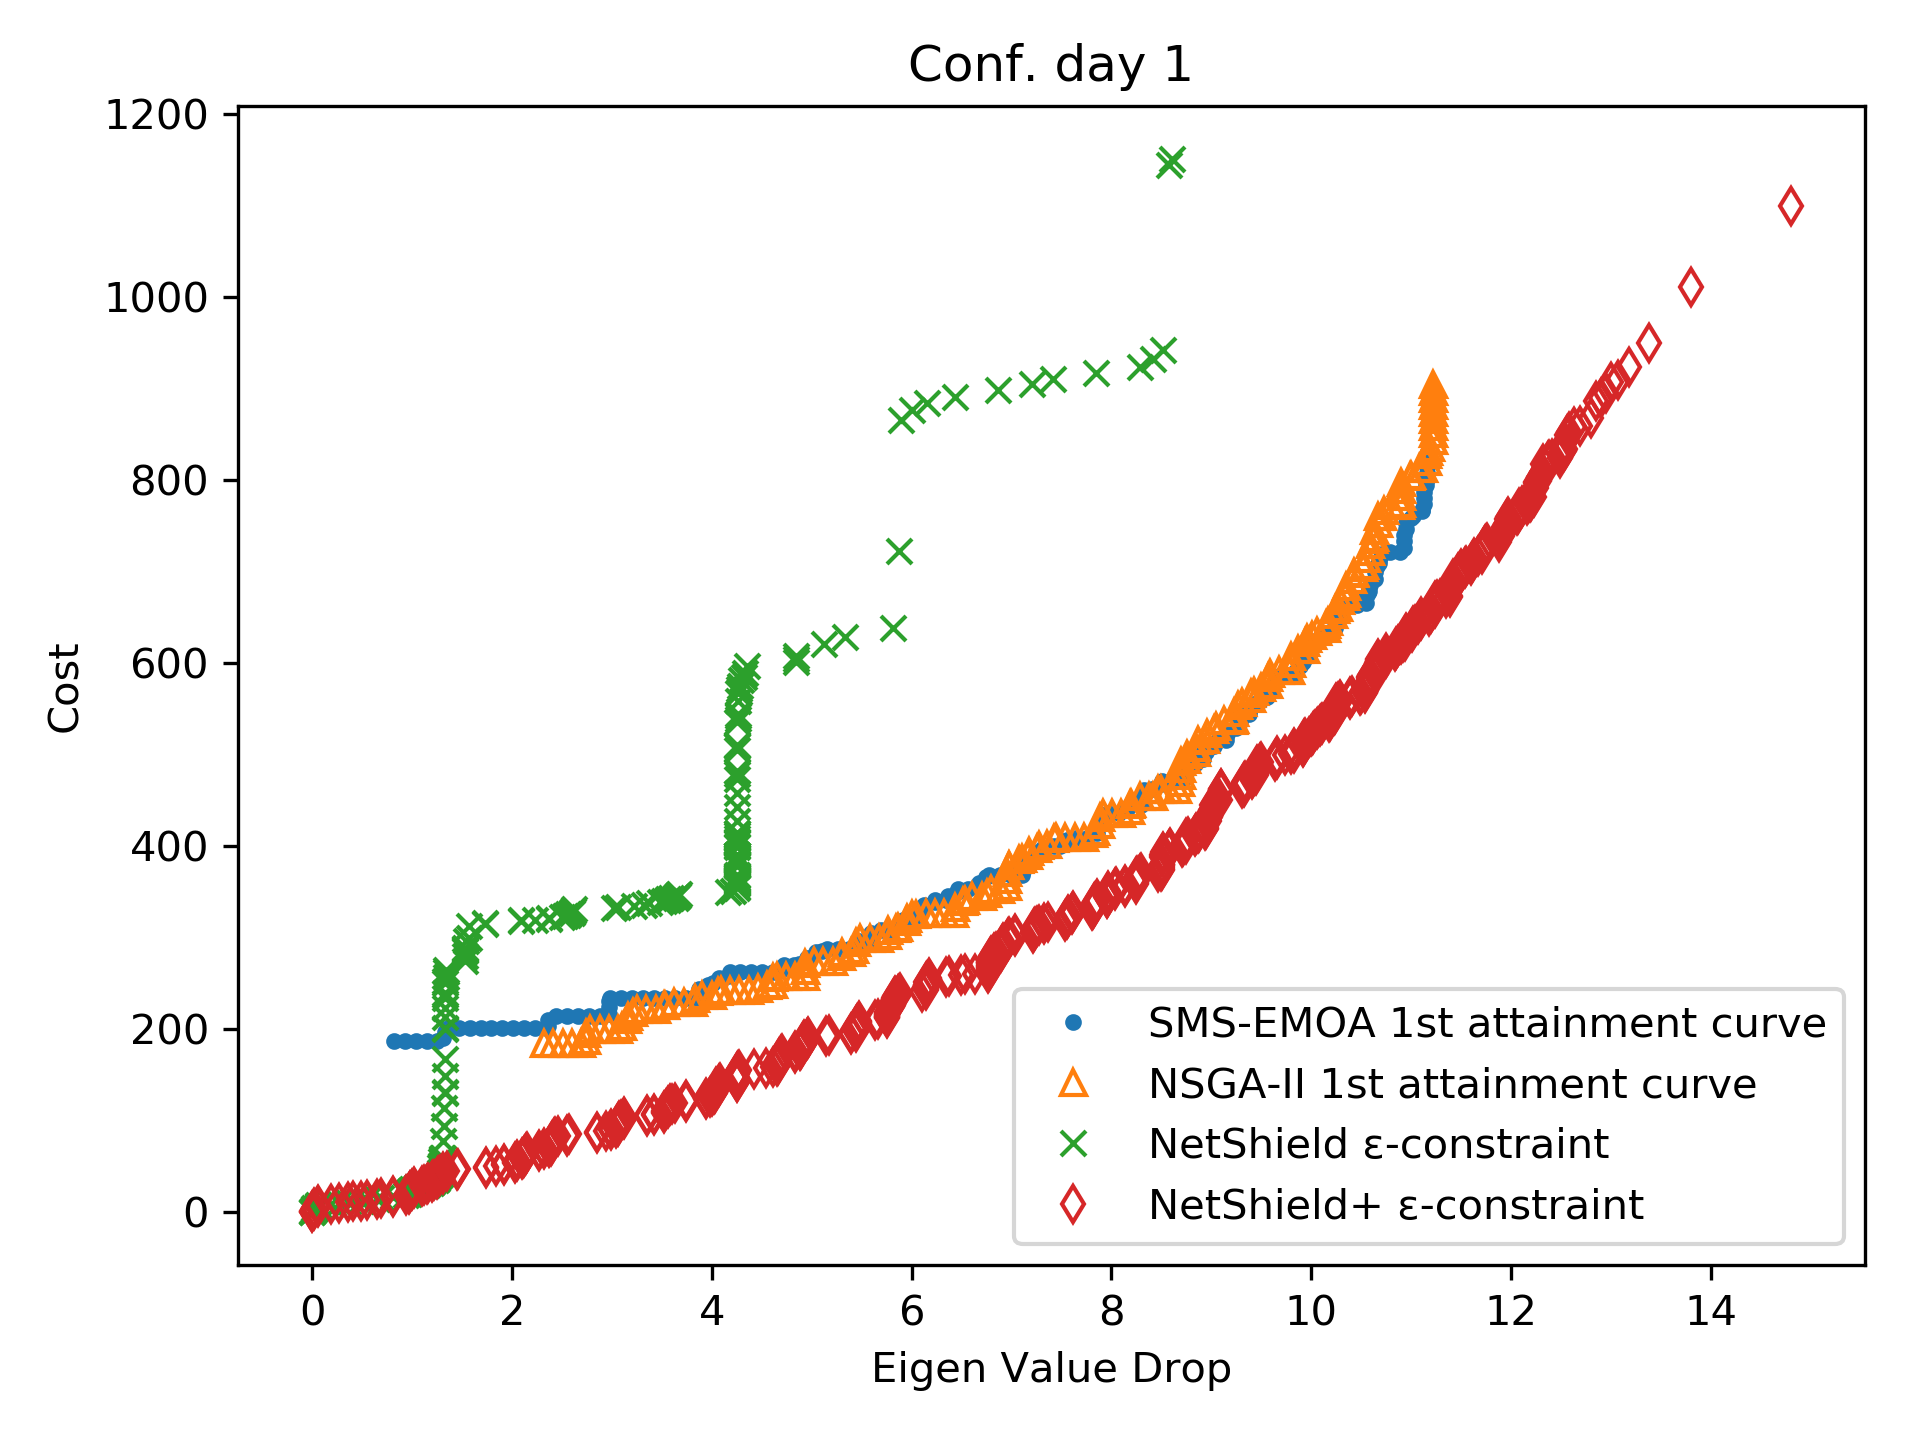
\includegraphics[width=0.75\textwidth]{results_ns_ga/day1_attaintment_netshield}
  \caption{Pareto front approximations of the GAs and NetShield(+) with $\epsilon$-constraint methods for the Conference Day 1 graph}
  \label{fig:day1_atns}
\end{figure}

\begin{figure}[h!]
  \centering
    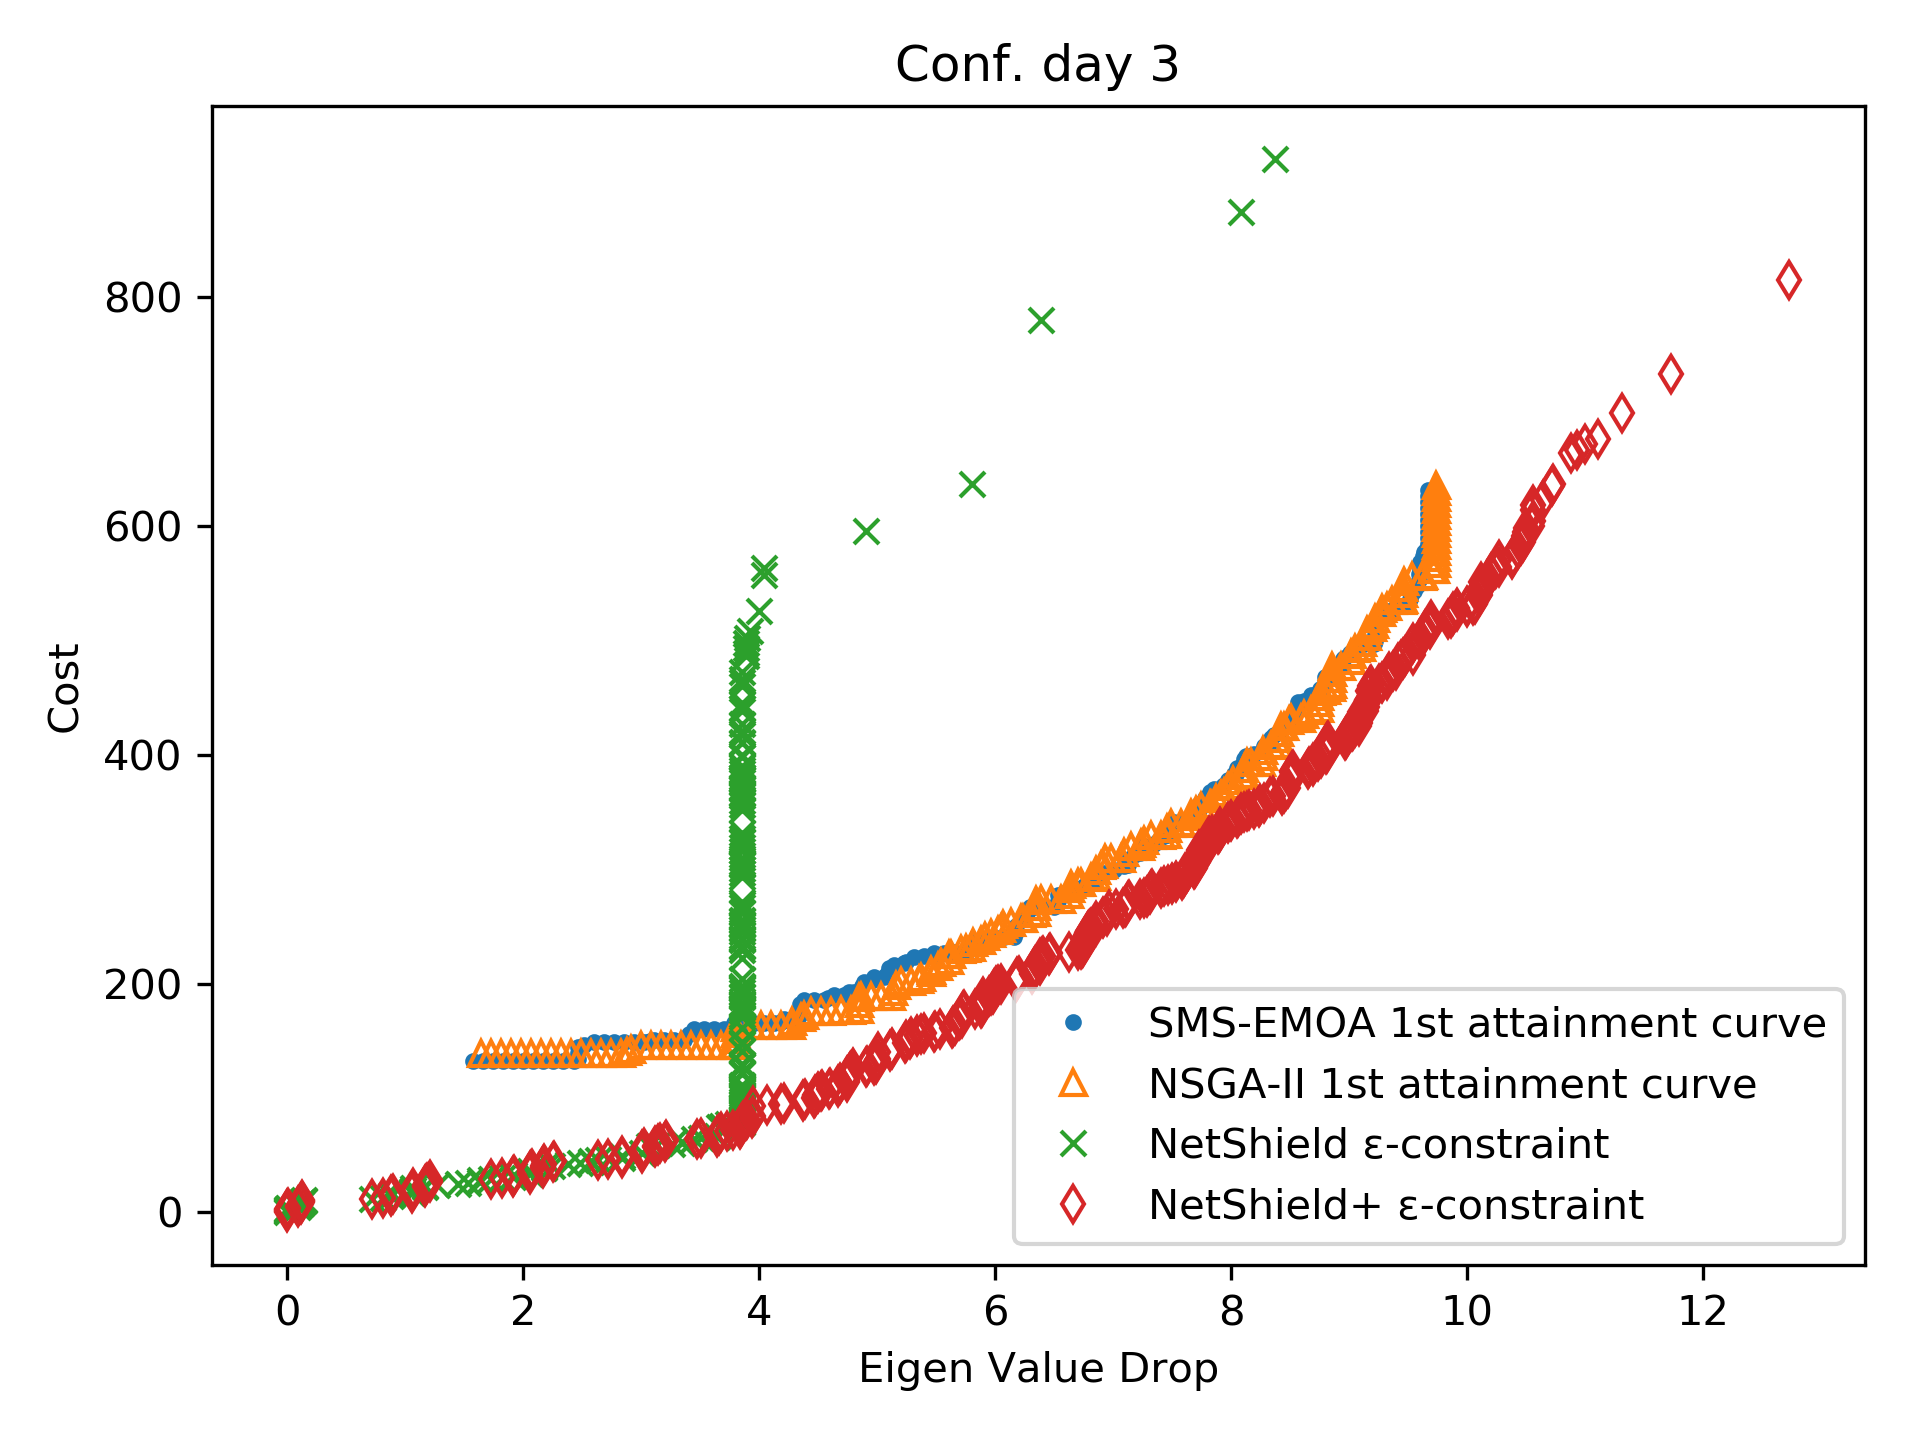
\includegraphics[width=0.75\textwidth]{results_ns_ga/day3_attaintment_netshield}
  \caption{Pareto front approximations of the GAs and NetShield(+) with $\epsilon$-constraint methods for the Conference Day 3 graph}
  \label{fig:day3_atns}
\end{figure}

\begin{figure}[h!]
  \centering
    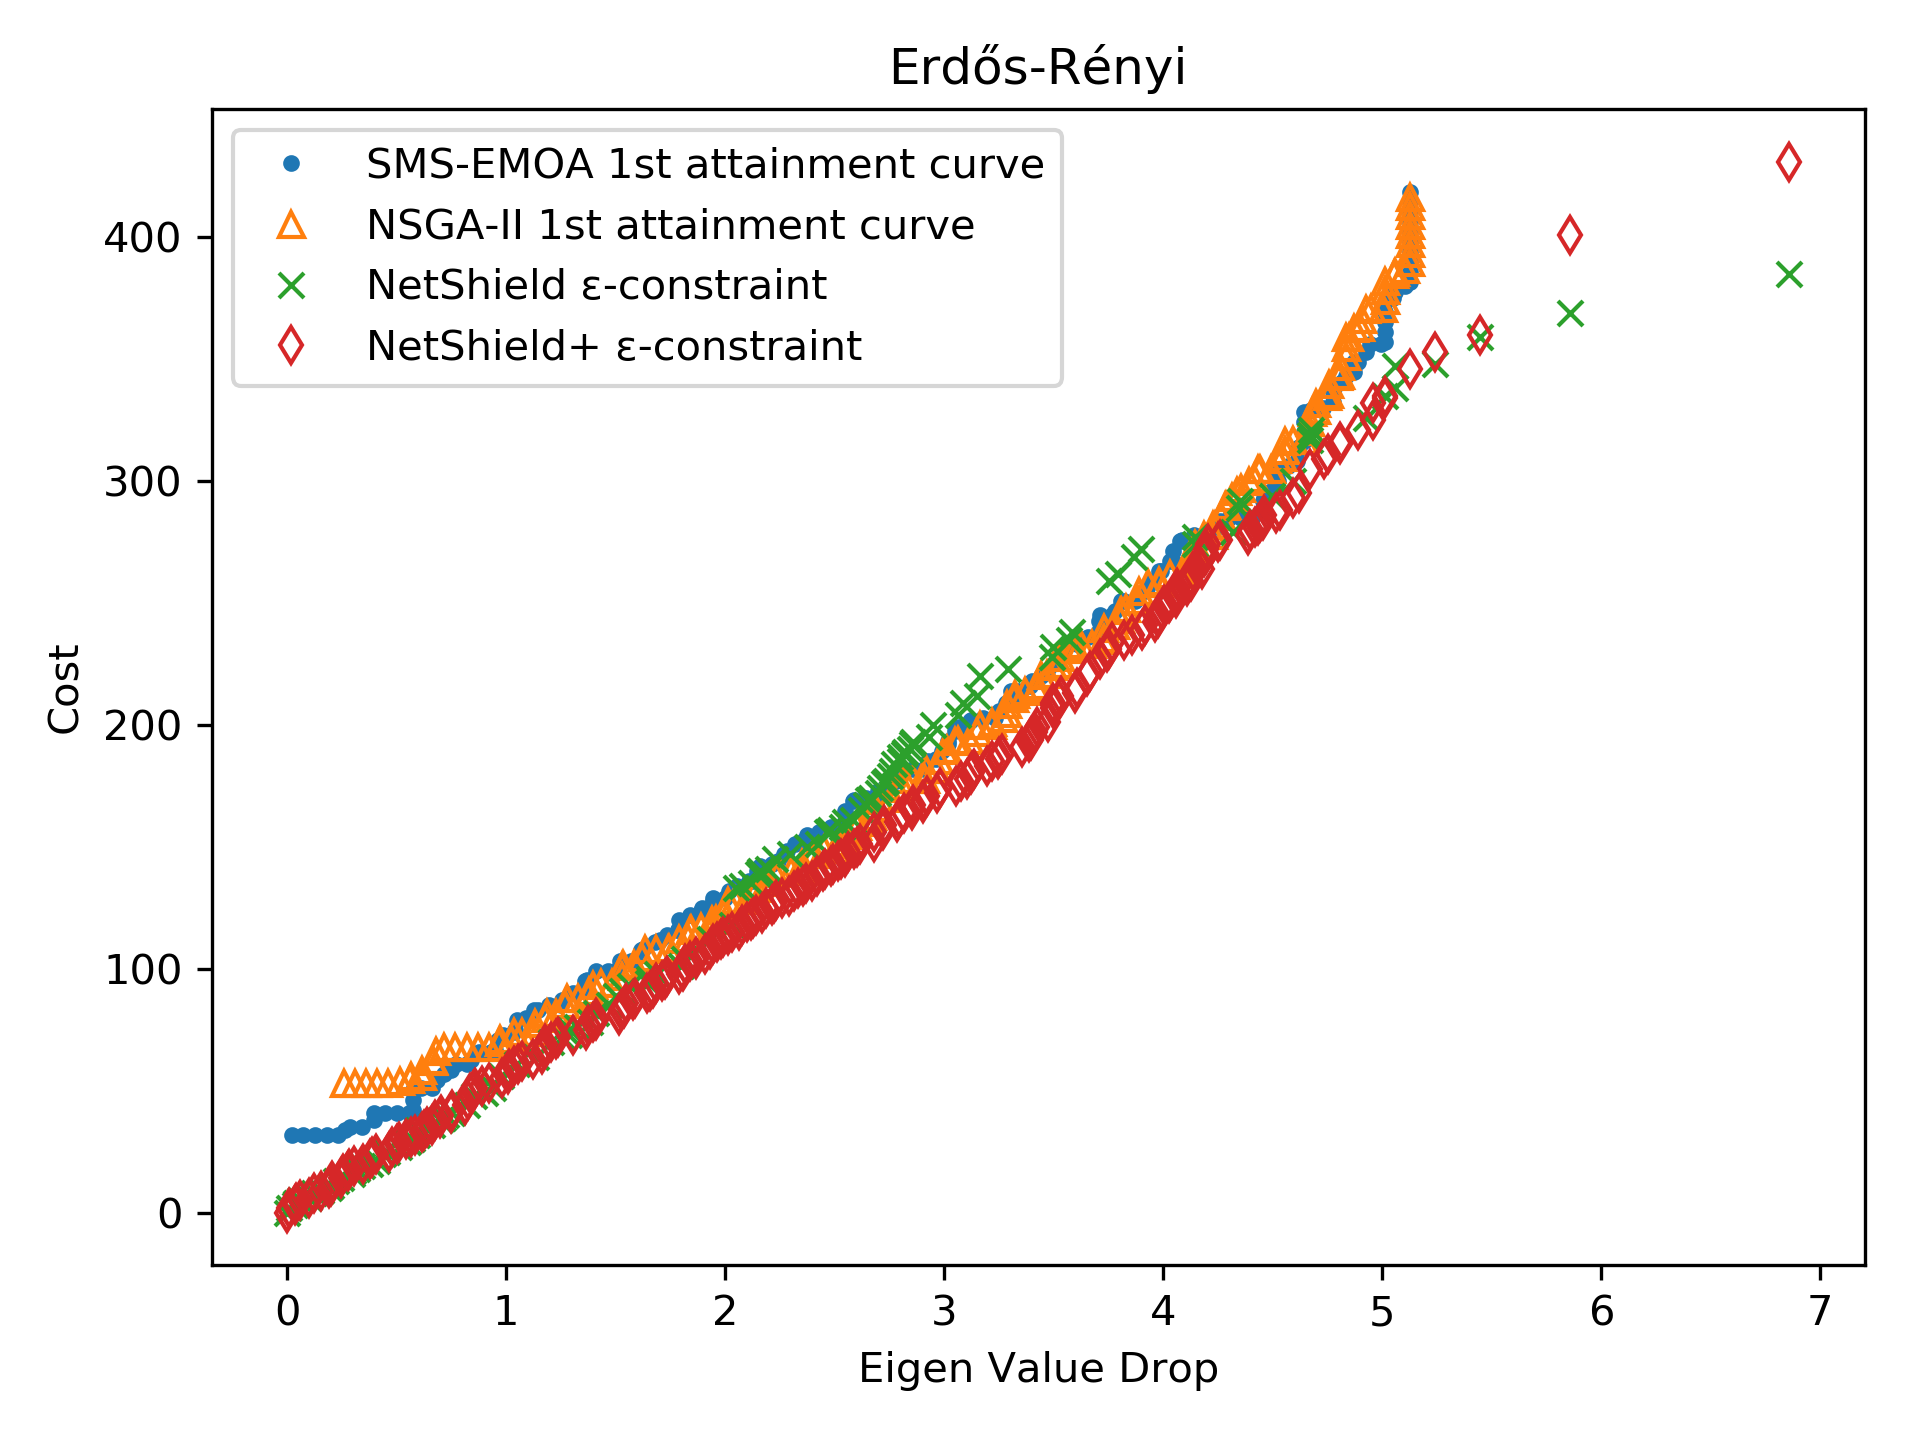
\includegraphics[width=0.75\textwidth]{results_ns_ga/Erdos_Renyi_V100_attaintment_netshield}
  \caption{Pareto front approximations of the GAs and NetShield(+) with $\epsilon$-constraint methods for the Erd\H{o}s-R\'enyi graph}
  \label{fig:erdos_renyi_atns}
\end{figure}

\begin{figure}[h!]
  \centering
    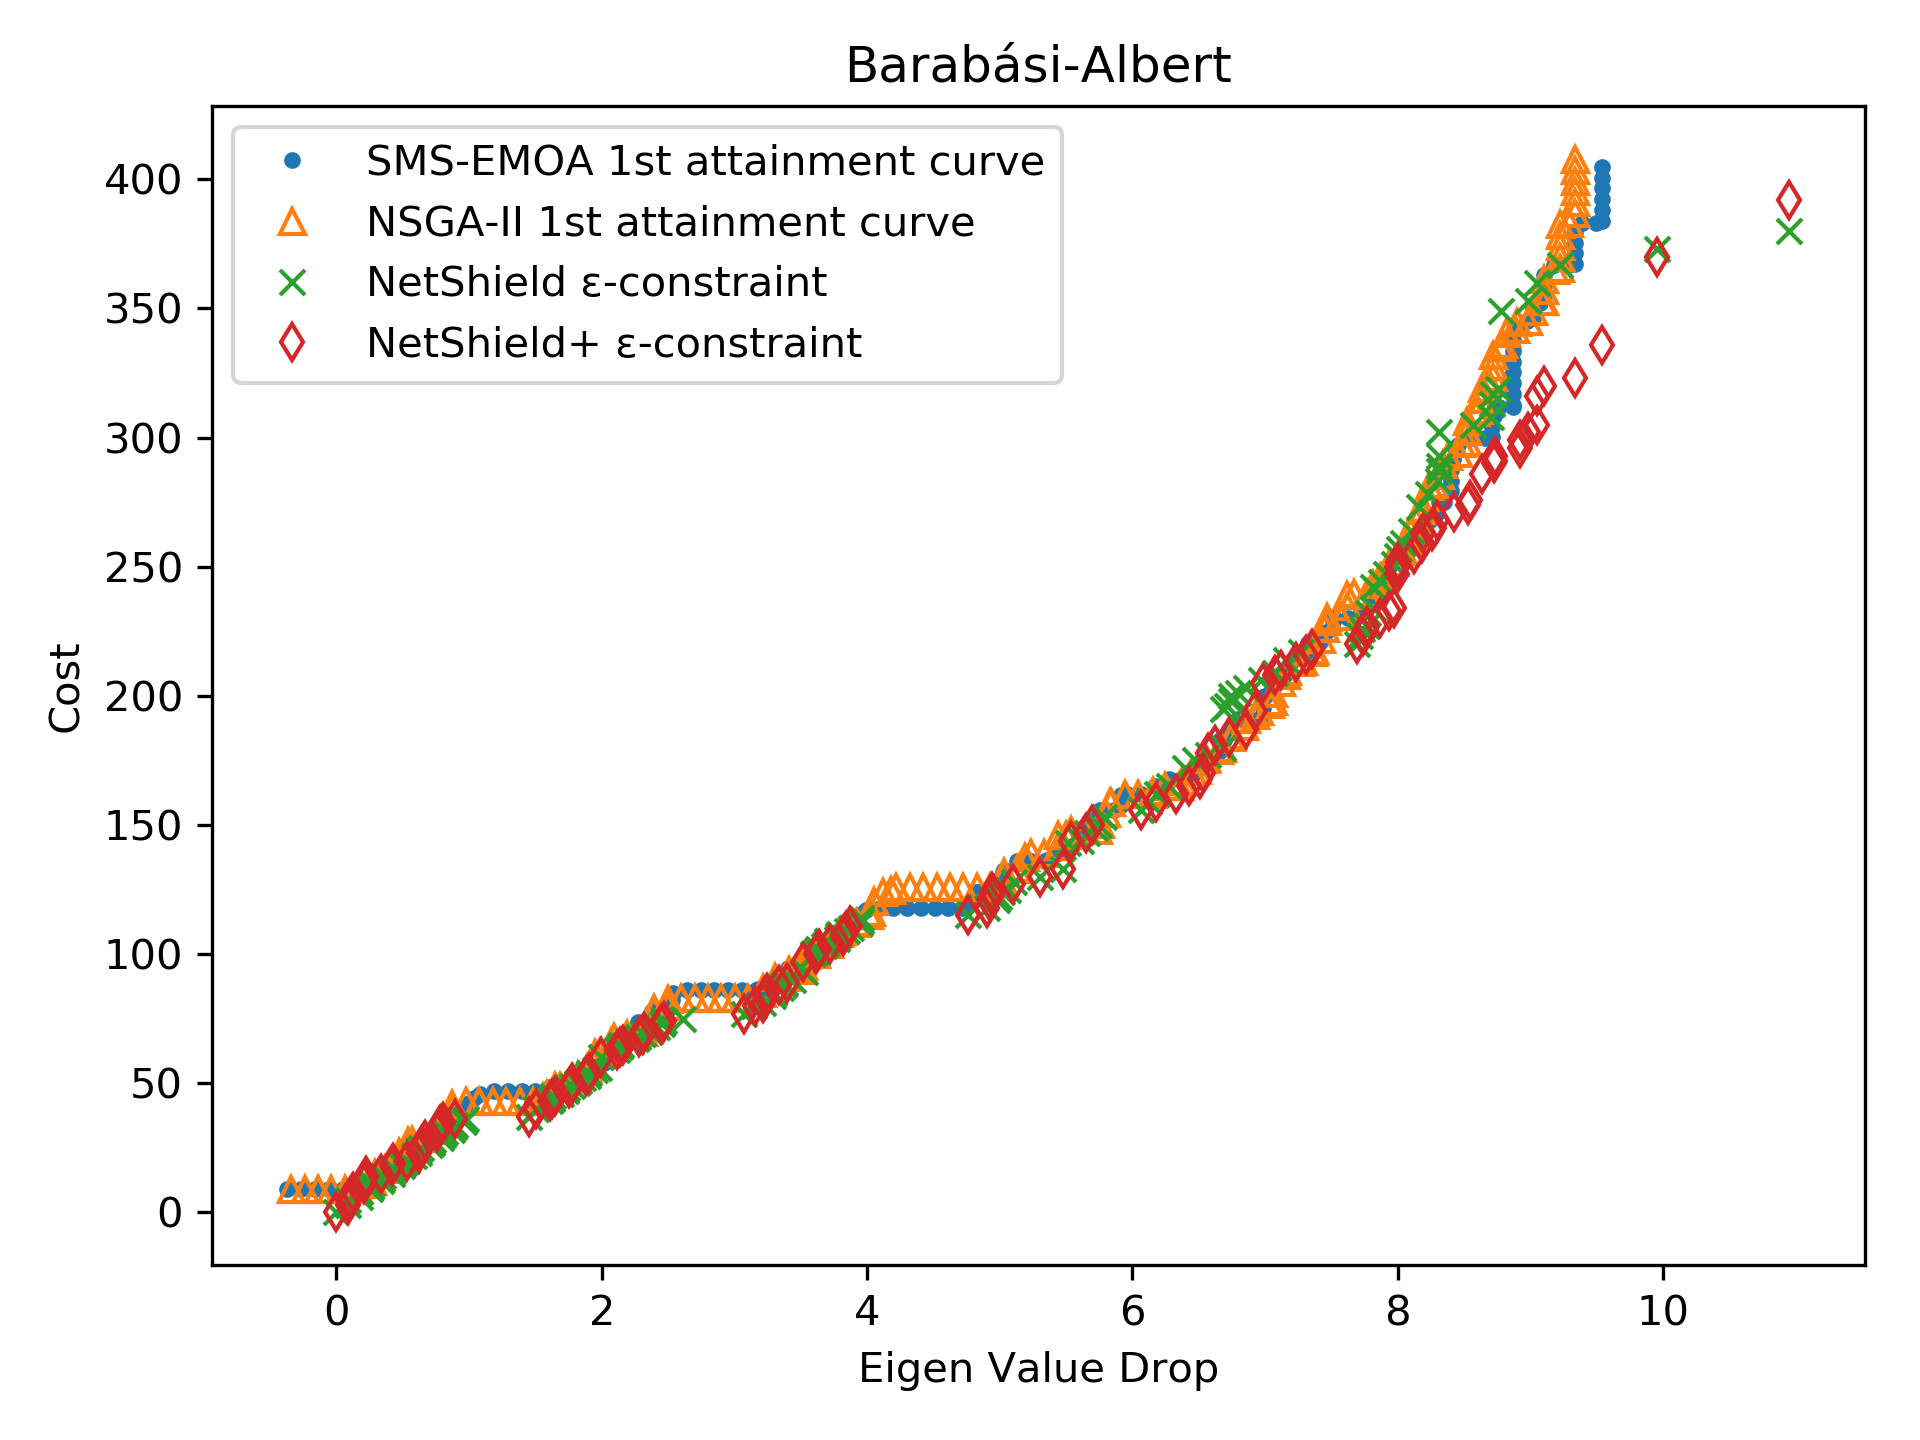
\includegraphics[width=0.75\textwidth]{results_ns_ga/Barabasi_Albert_V100_attaintment_netshield}
  \caption{Pareto front approximations of the GAs and NetShield(+) with $\epsilon$-constraint methods for the Barab\'asi-Albert graph}
  \label{fig:baral_atns}
\end{figure}

\begin{figure}[h!]
  \centering
    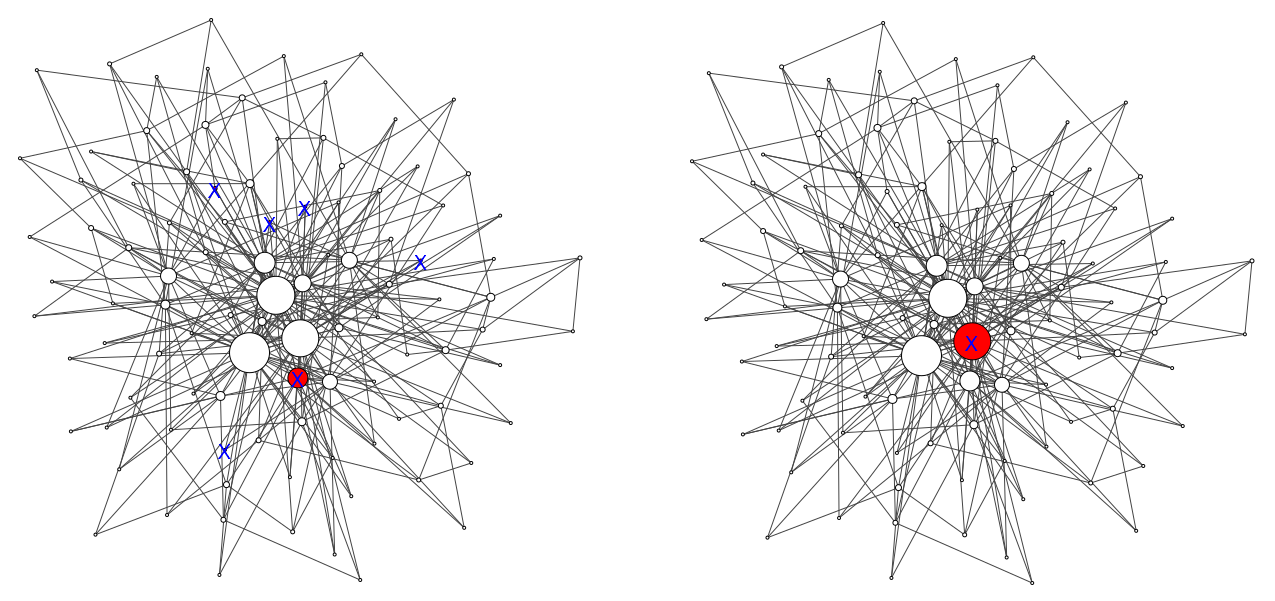
\includegraphics[width=1\textwidth]{other_img/j1}
  \caption{Example of large eigen-drop gain with small increase in cost for the Barab\'asi-Albert graph. 
    Left: 6 selected nodes, cost of 36, $\Delta\lambda$ of 0.975. 
    Right: 1 selected node, cost of 37, $\Delta\lambda$ of 1.455}
  \label{fig:j1}
\end{figure}

\begin{figure}[h!]
  \centering
    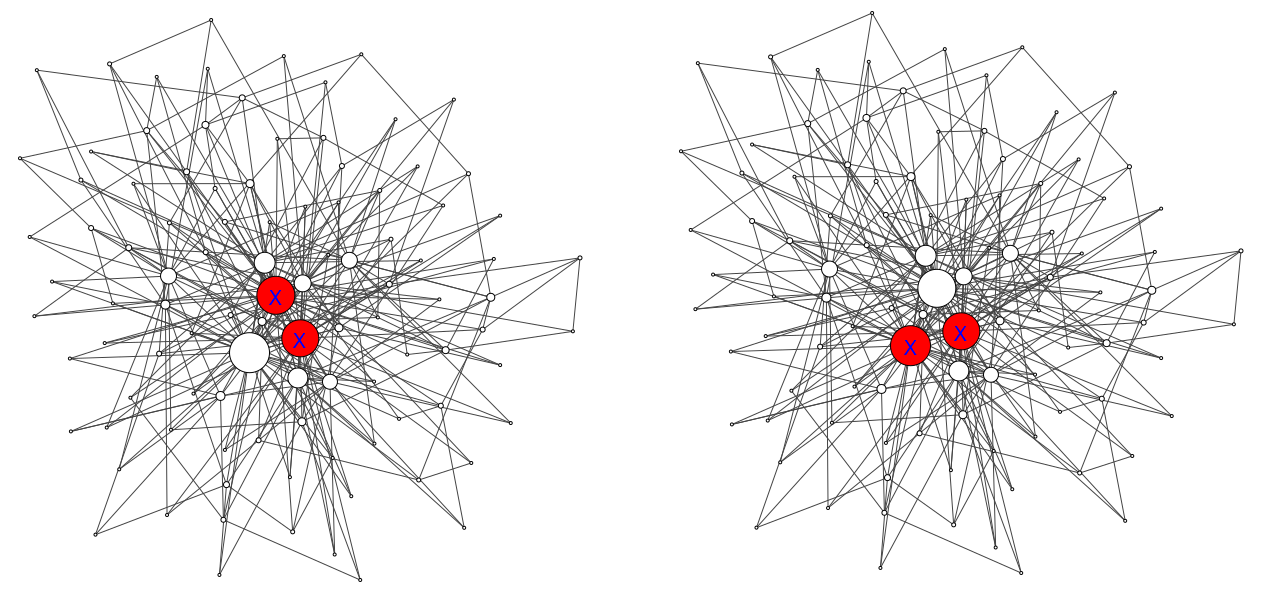
\includegraphics[width=1\textwidth]{other_img/j2}
  \caption{Example of large eigen-drop gain with small increase in cost for the Barab\'asi-Albert graph.
    Left: 2 selected nodes, cost of 75, $\Delta\lambda$ of 2.615.
    Right: 2 selected nodes, cost of 77, $\Delta\lambda$ of 3.069}
  \label{fig:j2}
\end{figure}

\begin{figure}[h!]
  \centering
    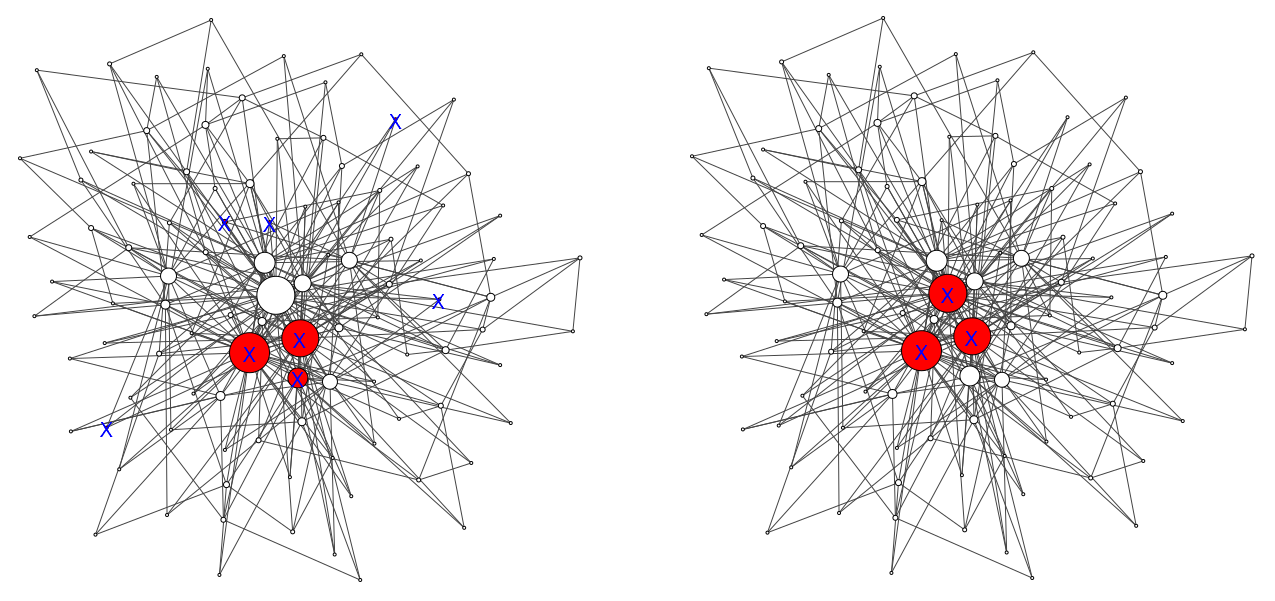
\includegraphics[width=1\textwidth]{other_img/j3}
  \caption{
    Example of large eigen-drop gain with small increase in cost for the Barab\'asi-Albert graph.
    Left: 8 selected nodes, cost of 75, $\Delta\lambda$ of 3.955.
    Right: 3 selected nodes, cost of 77, $\Delta\lambda$ of 4.979}
  \label{fig:j3}
\end{figure}

\clearpage

\subsubsection{Hybrid GA approach}

For the hybrid approach, the GAs were initialised with the results from the NetShield methods. The initialisation sets were created by combining the solutions found by both NetShield methods and filtering out the dominated solutions. The results given are again the first attainment curves. They are shown together with the initialisation sets in Figures \ref{fig:karate_atins} to \ref{fig:baral_atins}. In all cases, improvements have been made when compared to the initialisation sets. These improvements however, are consistently minor. Either the initialisation sets are already close to the Pareto fronts or there may not be enough diversity in the initial populations for the GAs to find better solutions.

The most notable improvements found by the GAs are for the Pandemic graph shown in figure \ref{fig:Pandemic_atins}. Here the results of the inaccuracies of the Shield-value have been corrected. It appears that in these cases, the GAs have the ability to repair such issues. On the whole however, the benefits are most likely not enough to justify the time investment needed for running the GAs.

\begin{figure}[h!]
  \centering
    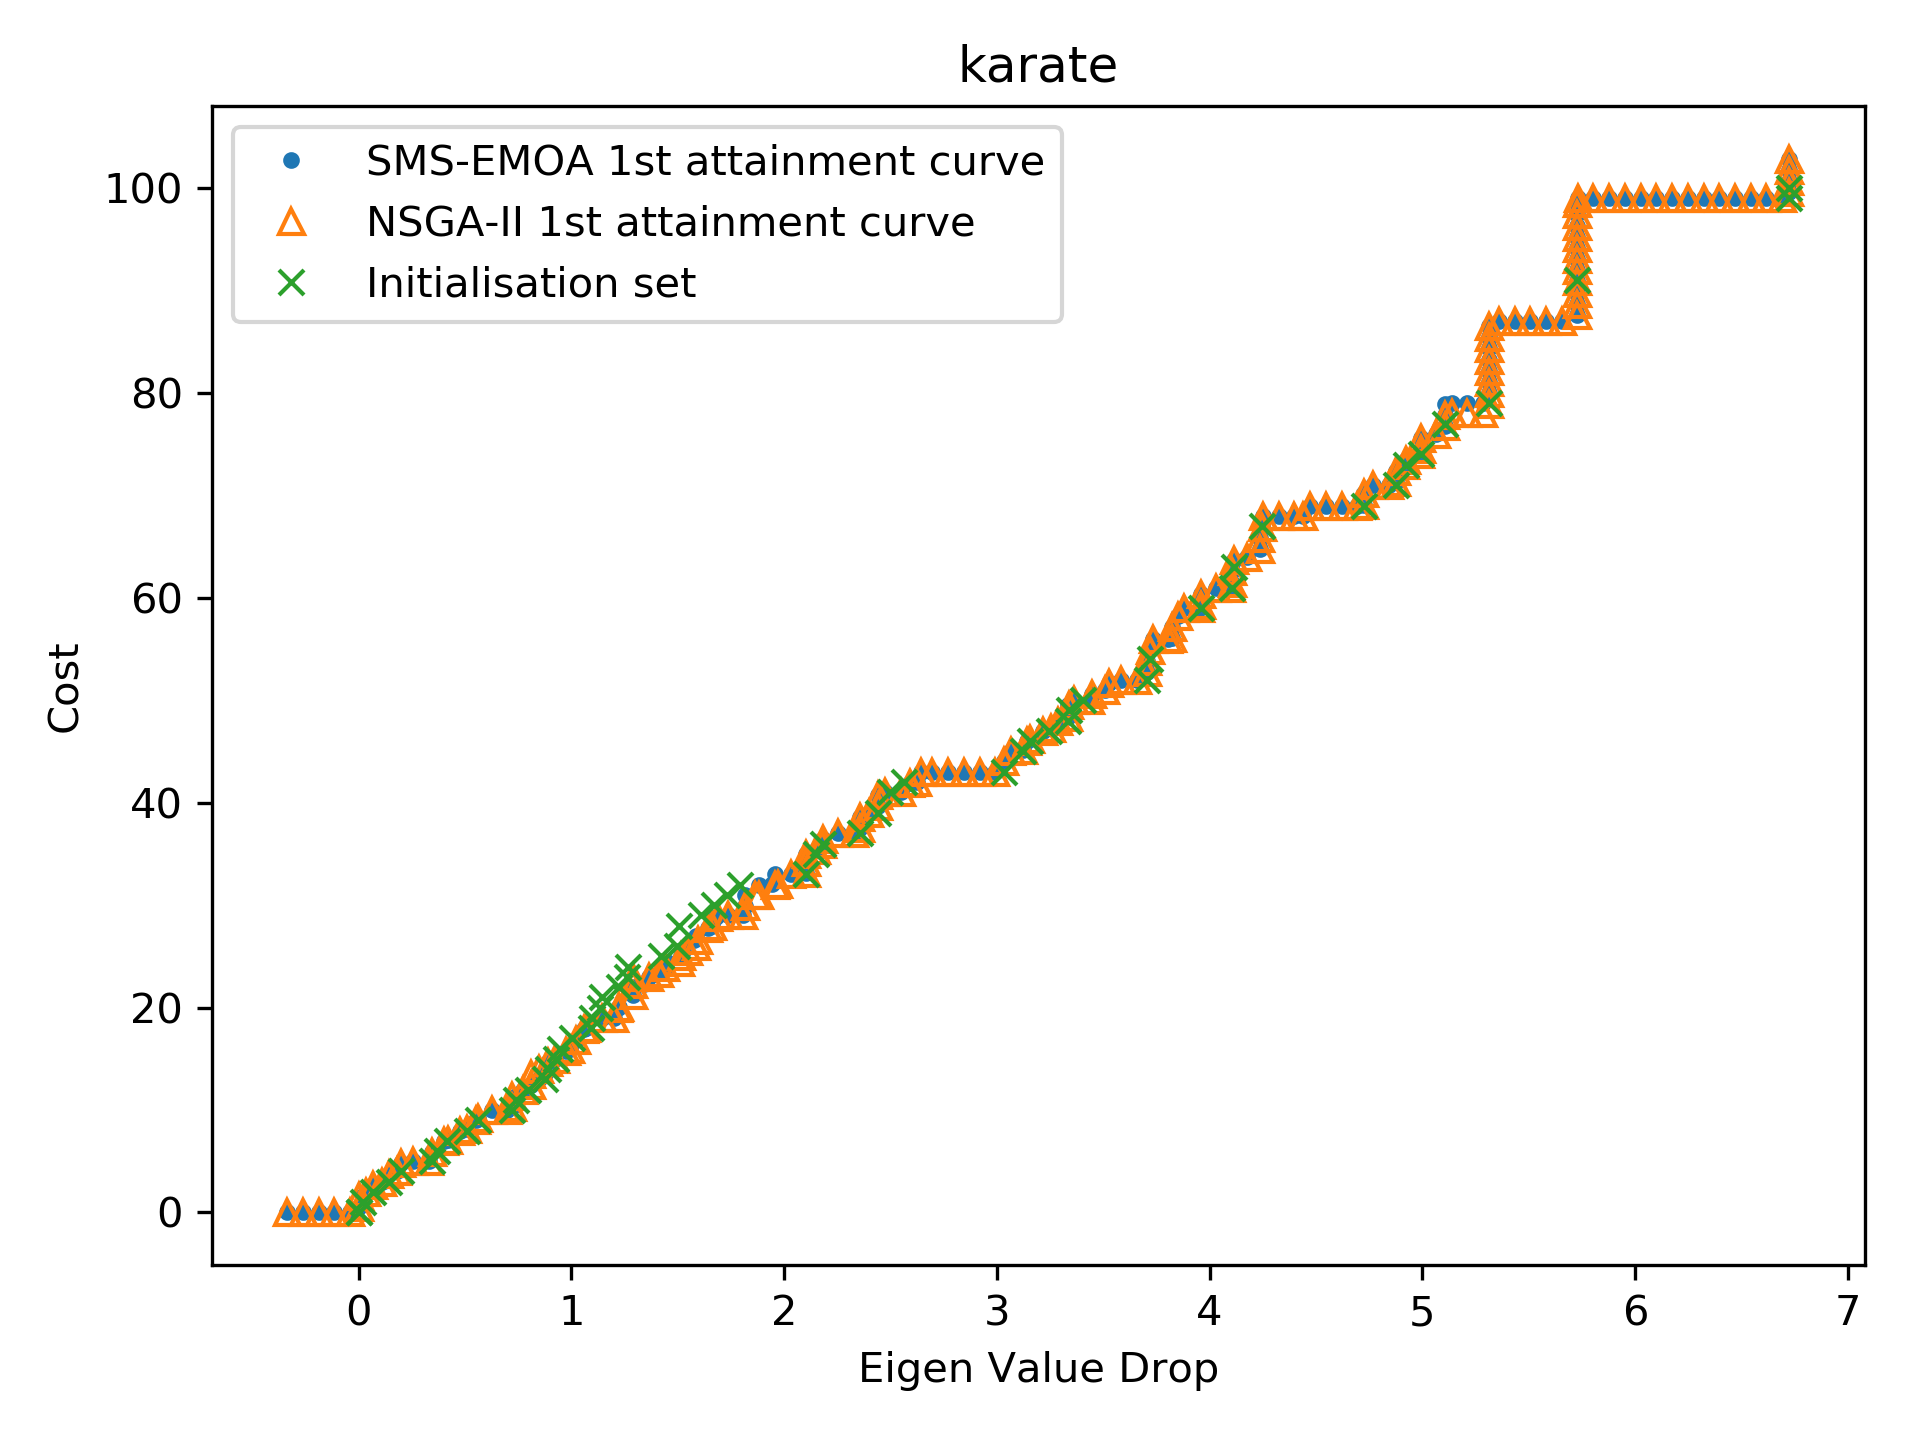
\includegraphics[width=0.75\textwidth]{results_ns_init/karate_attainment_nsinit}
  \caption{Pareto front approximation by the GAs and initialisation set based on NetShield and NetShield+ solutions for the karate graph}
  \label{fig:karate_atins}
\end{figure}

\begin{figure}[h!]
  \centering
    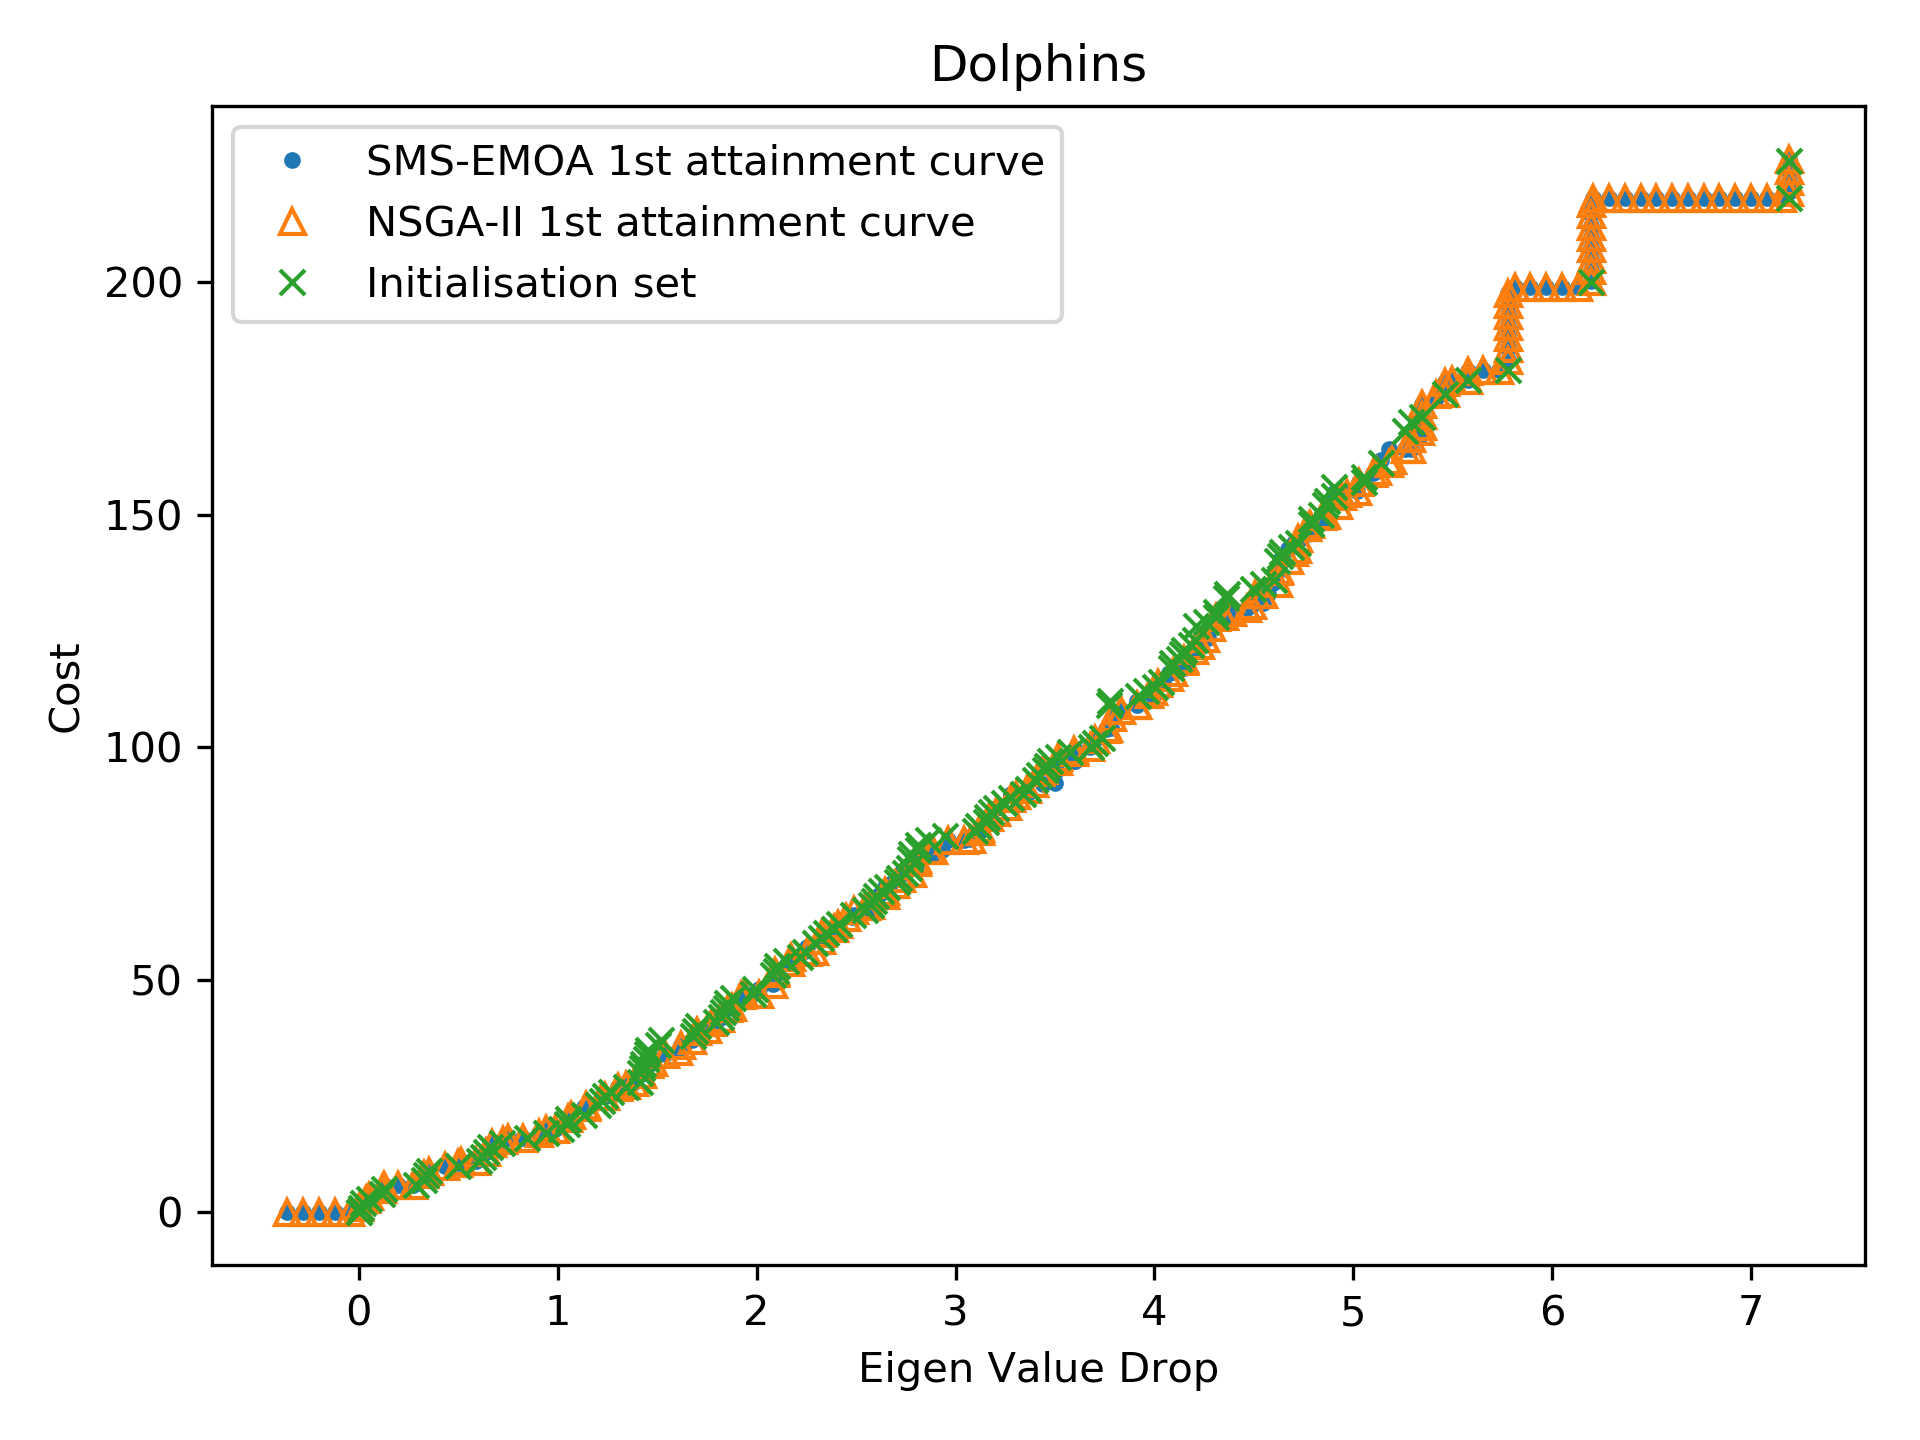
\includegraphics[width=0.75\textwidth]{results_ns_init/dolphins_attainment_nsinit}
  \caption{Pareto front approximation by the GAs and initialisation set based on NetShield and NetShield+ solutions for the Dolphin graph}
  \label{fig:dolphin_atins}
\end{figure}

\begin{figure}[h!]
  \centering
    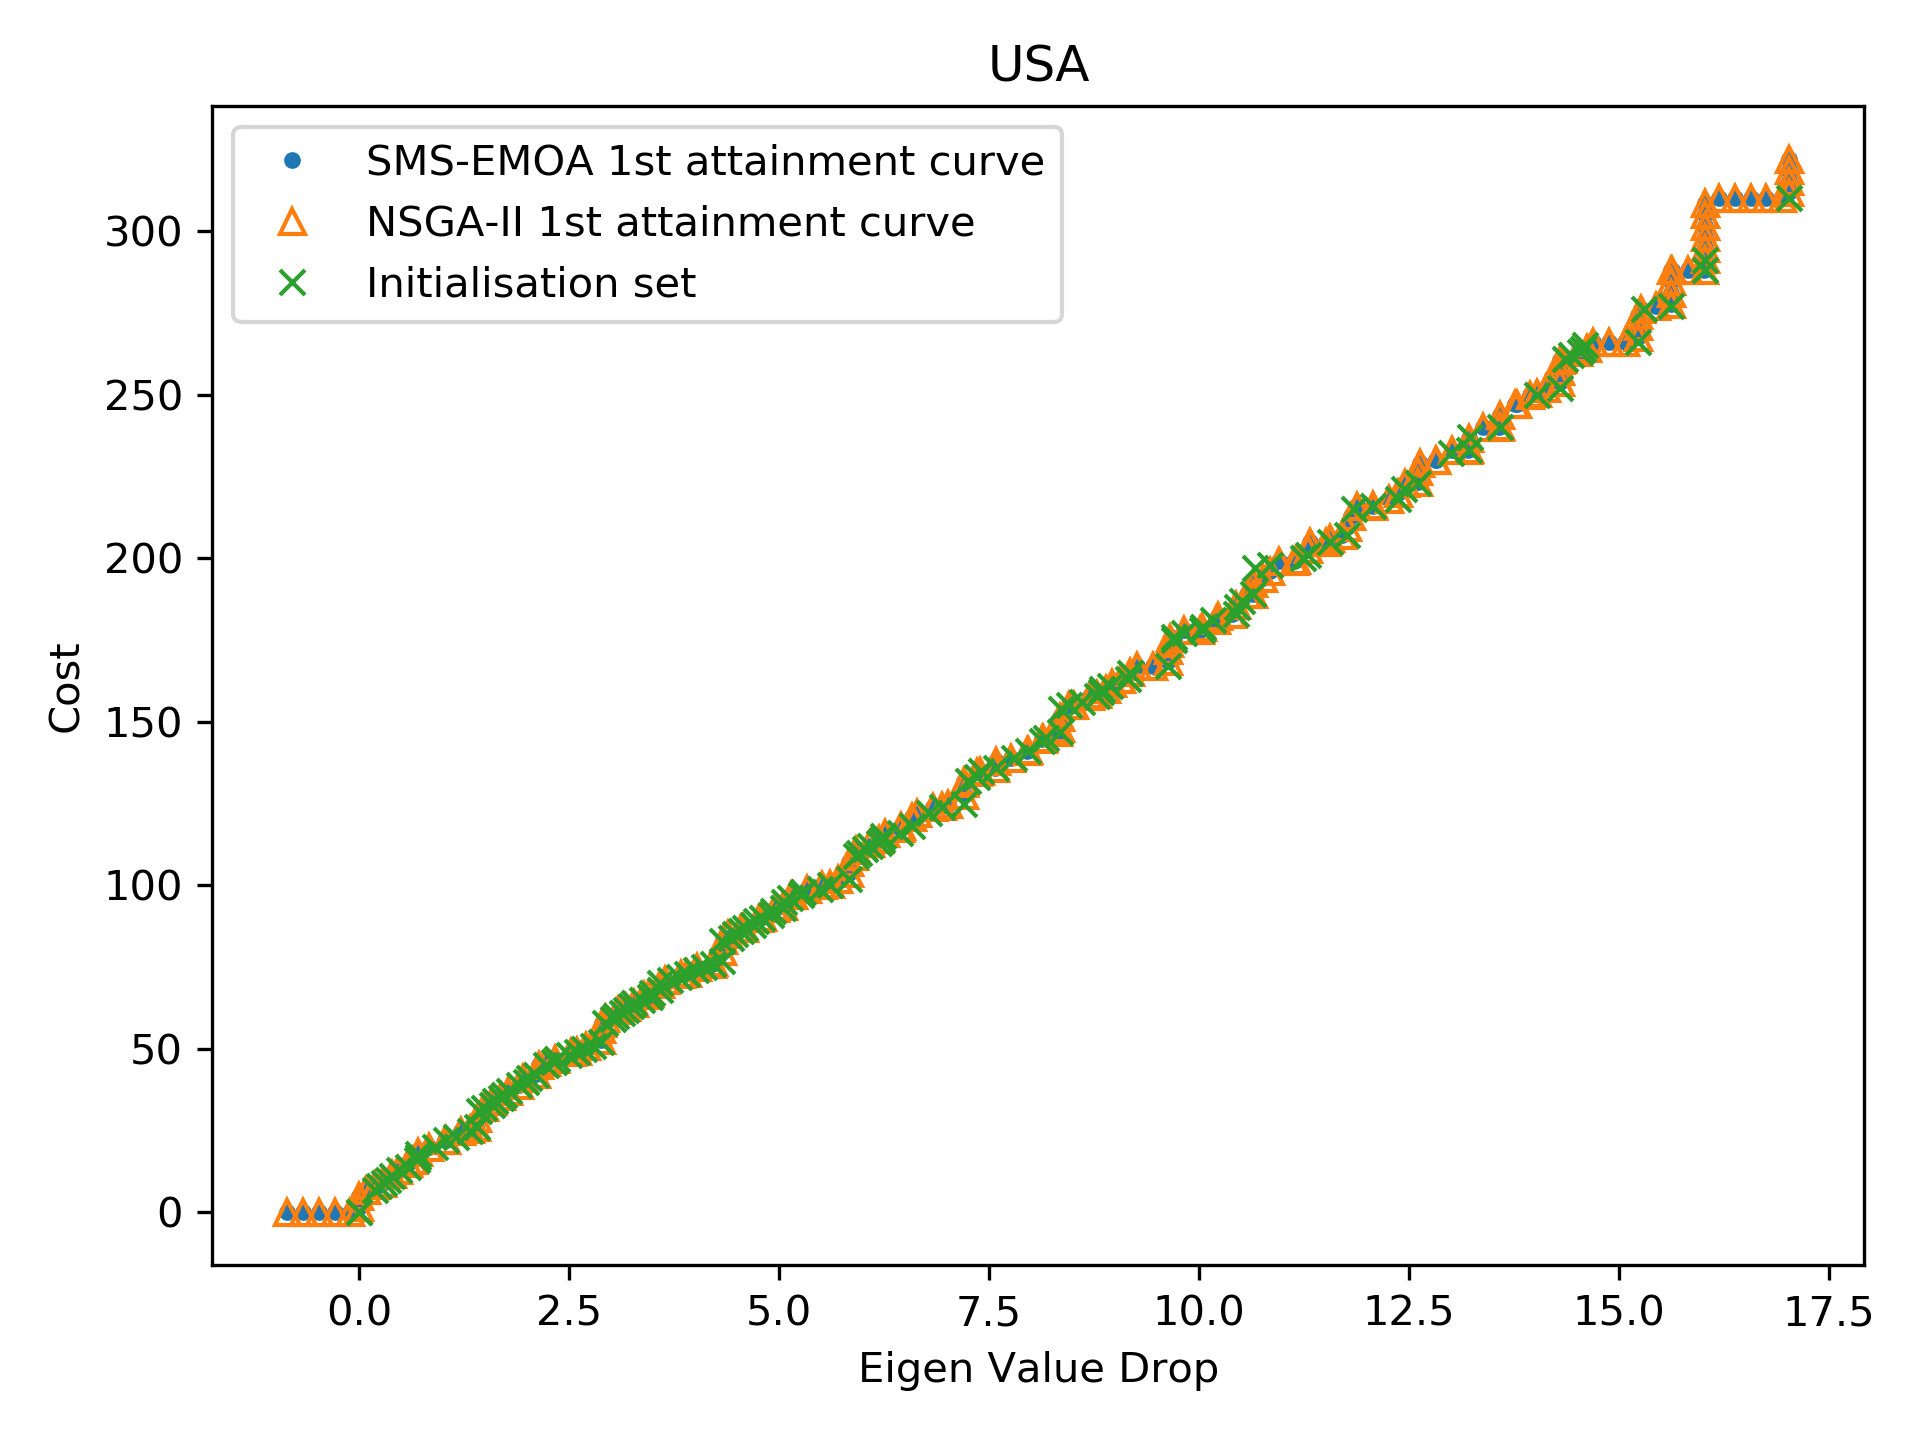
\includegraphics[width=0.75\textwidth]{results_ns_init/USA_attainment_nsinit}
  \caption{Pareto front approximation by the GAs and initialisation set based on NetShield and NetShield+ solutions for the USA graph}
  \label{fig:USA_atins}
\end{figure}

\begin{figure}[h!]
  \centering
    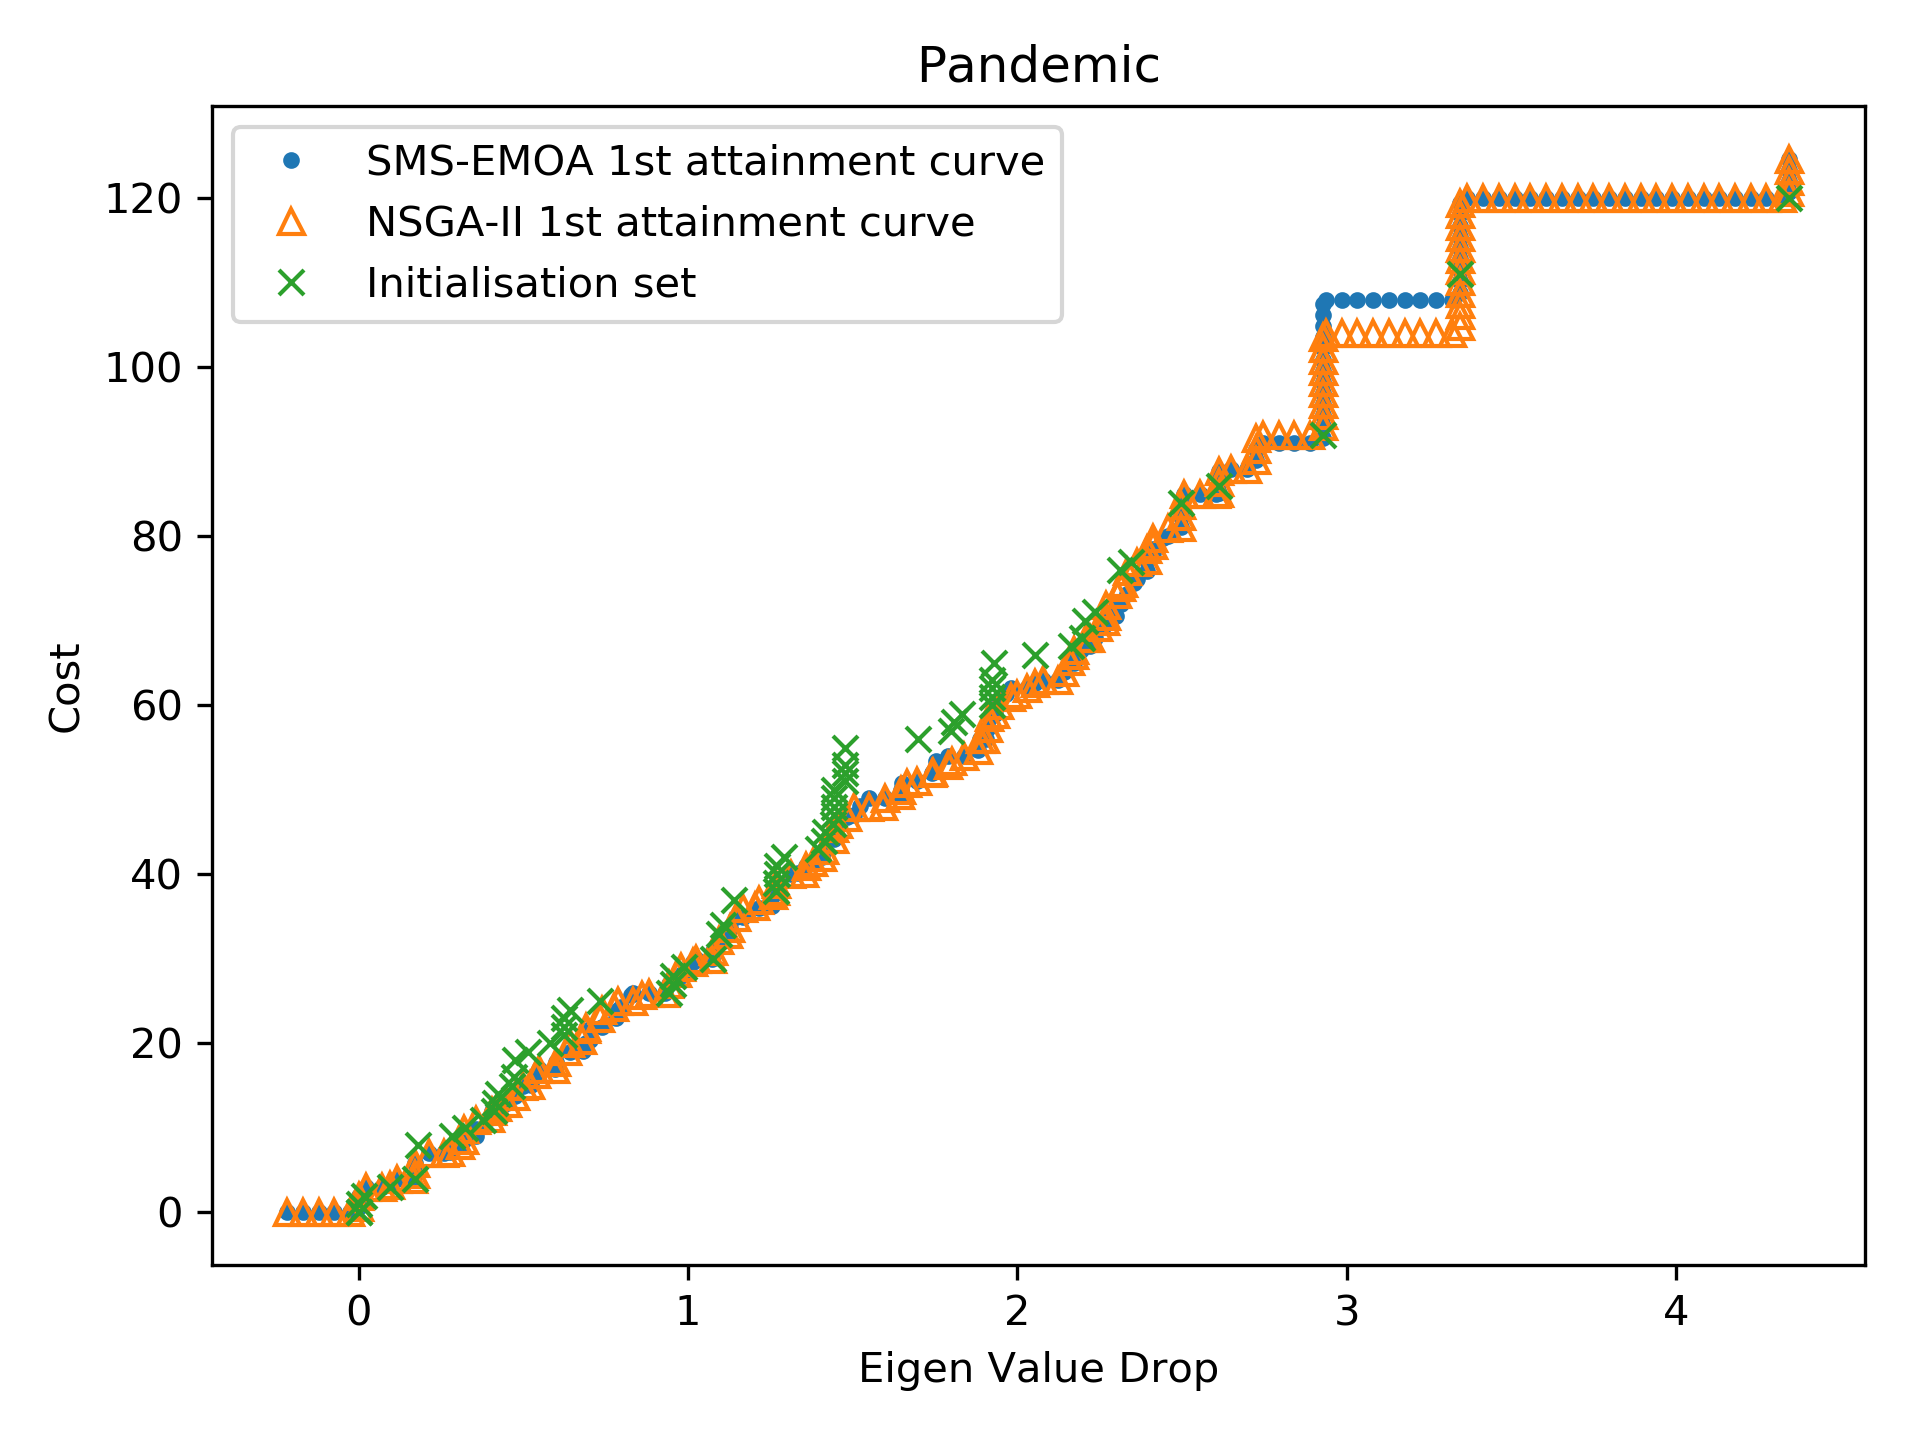
\includegraphics[width=0.75\textwidth]{results_ns_init/pandemic_attainment_nsinit}
  \caption{Pareto front approximation by the GAs and initialisation set based on NetShield and NetShield+ solutions for the Pandemic graph}
  \label{fig:Pandemic_atins}
\end{figure}

\begin{figure}[h!]
  \centering
    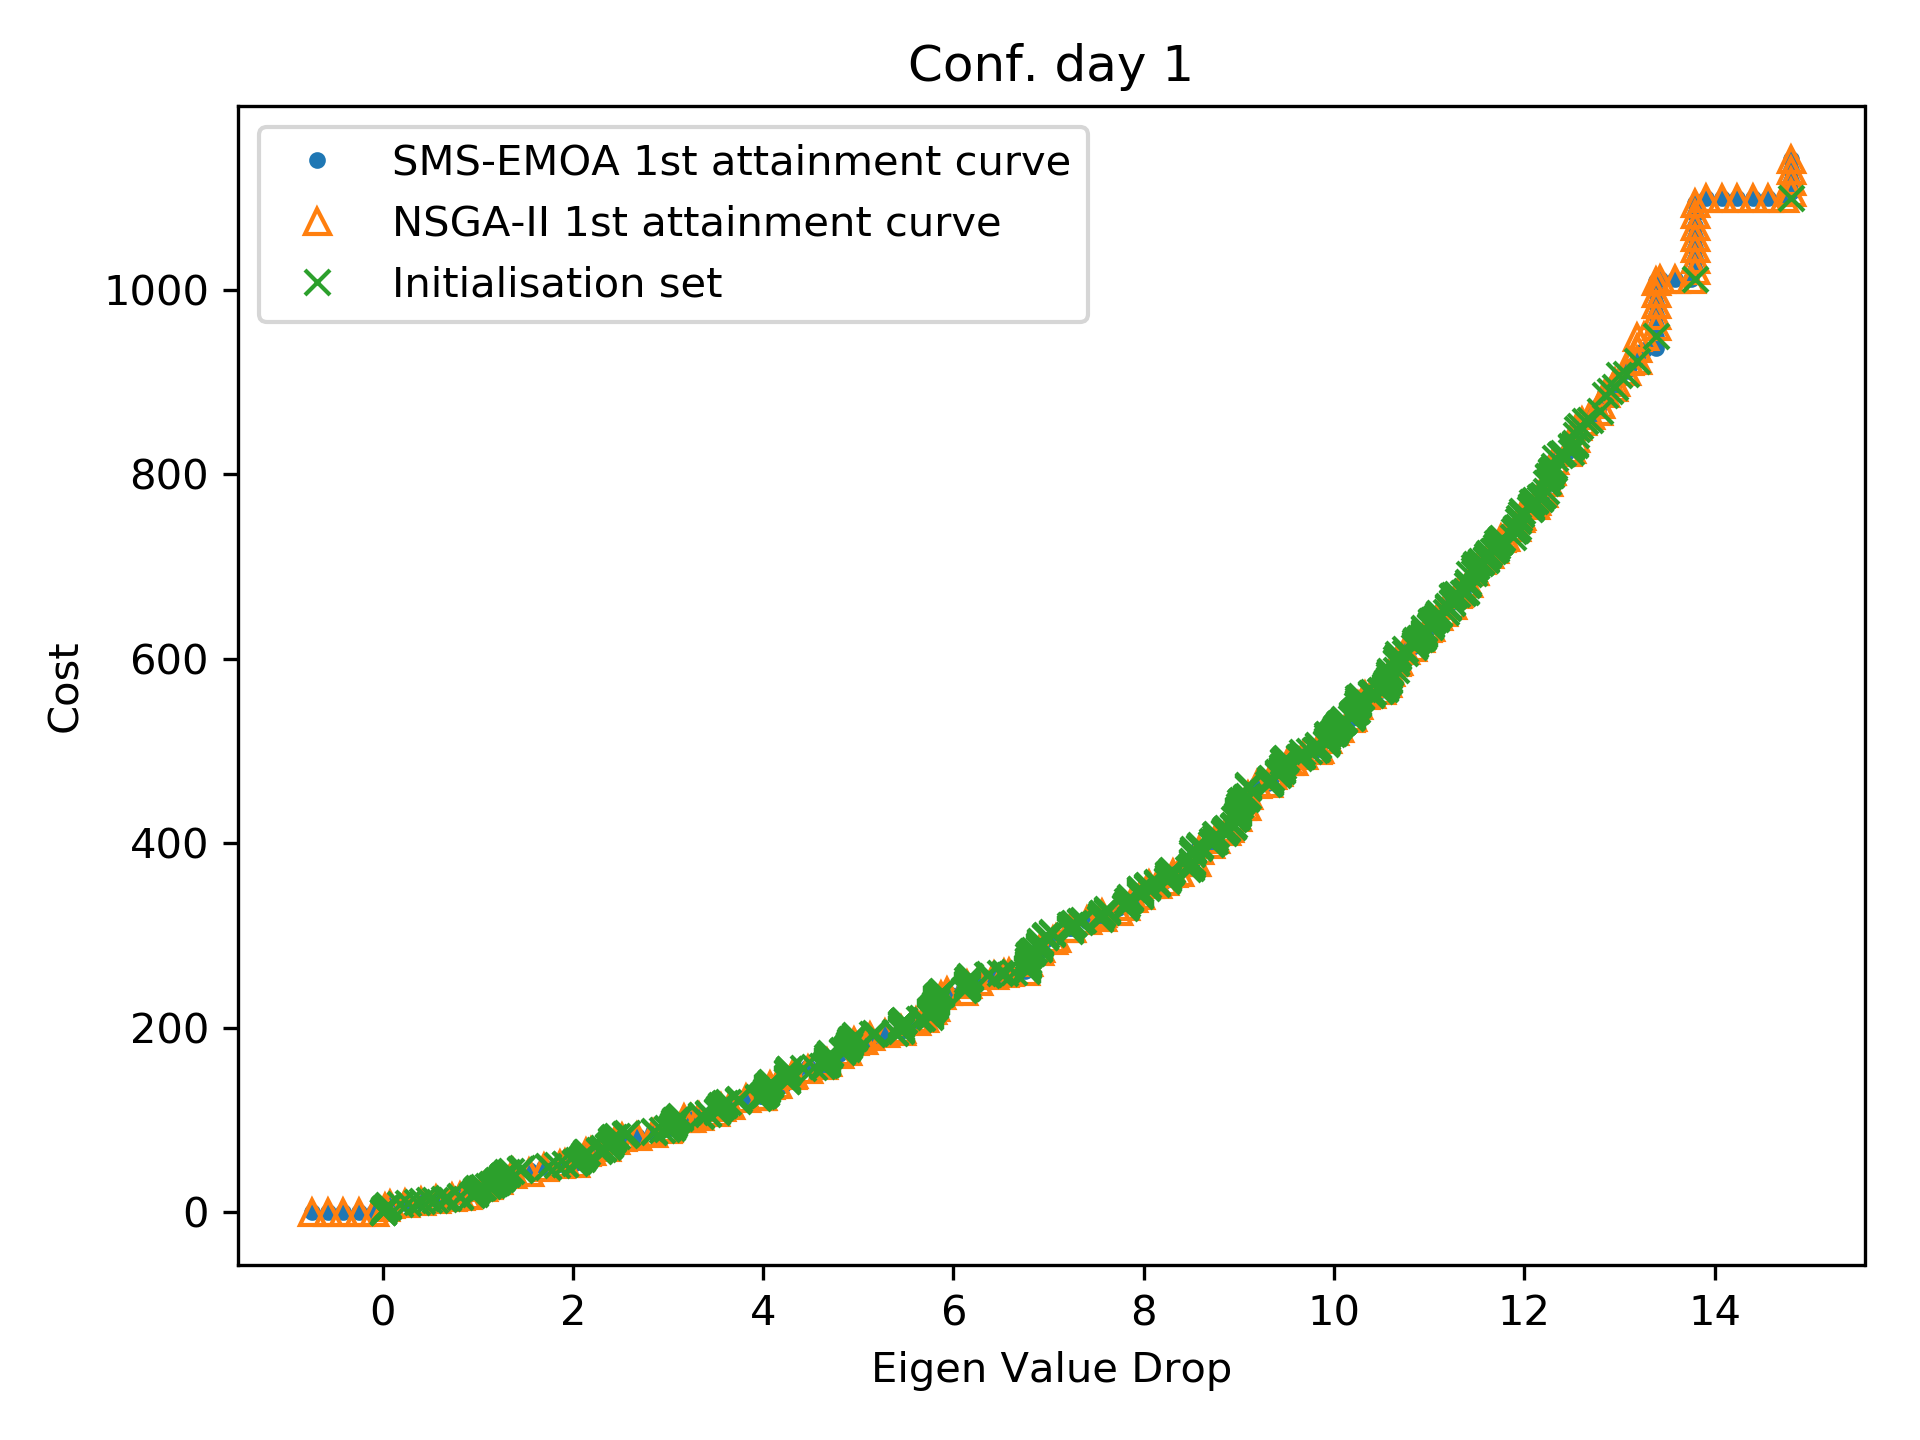
\includegraphics[width=0.75\textwidth]{results_ns_init/day1_attainment_nsinit}
  \caption{Pareto front approximation by the GAs and initialisation set based on NetShield and NetShield+ solutions for the Conference Day 1 graph}
  \label{fig:day1_atins}
\end{figure}

\begin{figure}[h!]
  \centering
    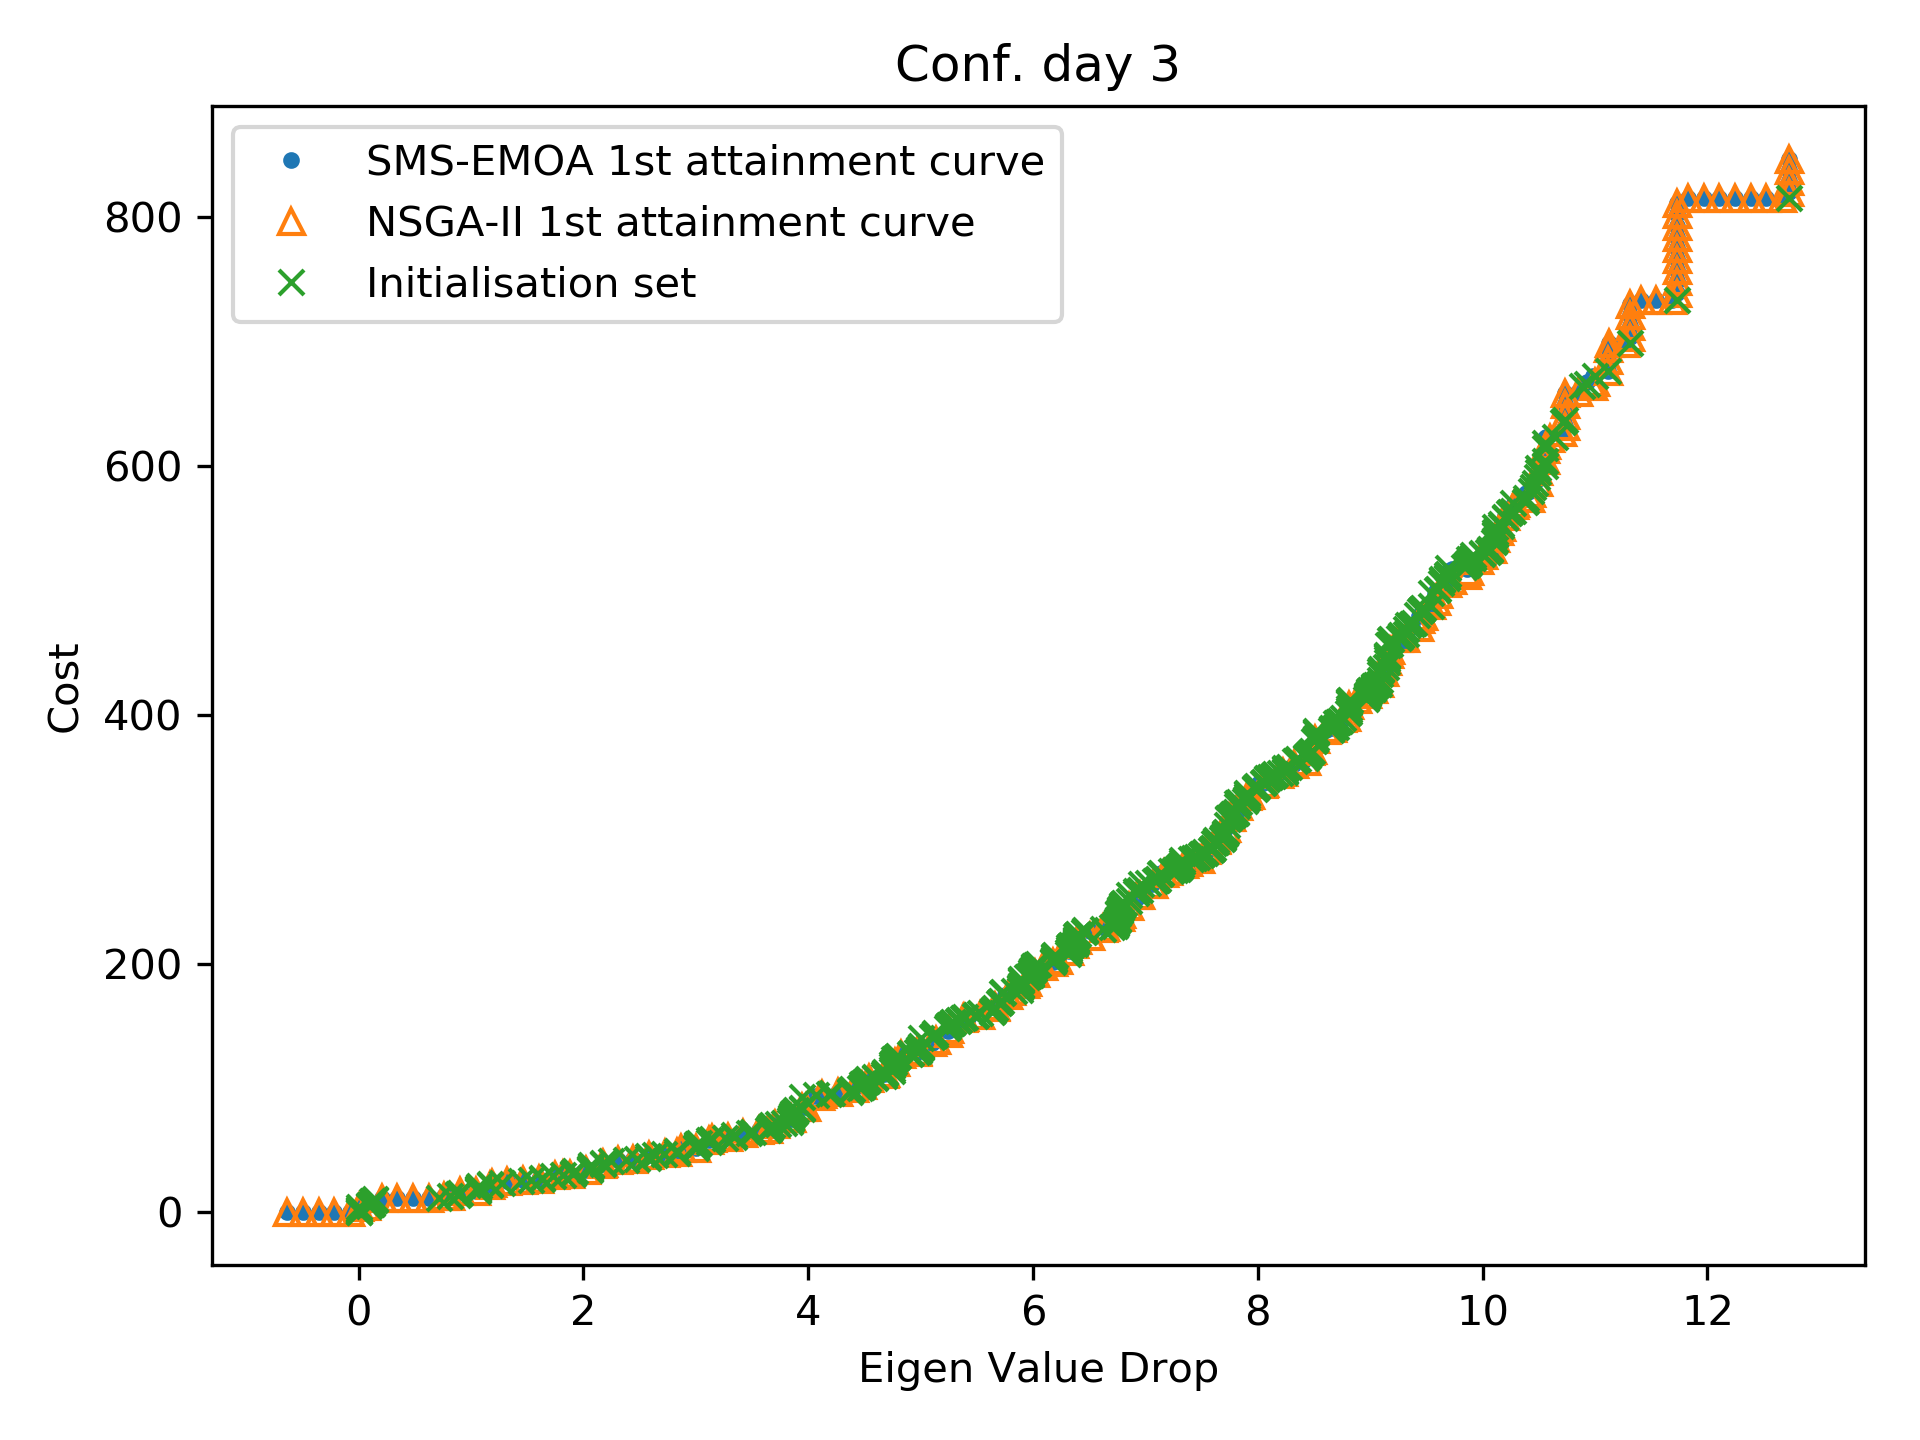
\includegraphics[width=0.75\textwidth]{results_ns_init/day3_attainment_nsinit}
  \caption{Pareto front approximation by the GAs and initialisation set based on NetShield and NetShield+ solutions for the Conference Day 2 graph}
  \label{fig:day3_atins}
\end{figure}

\begin{figure}[h!]
  \centering
    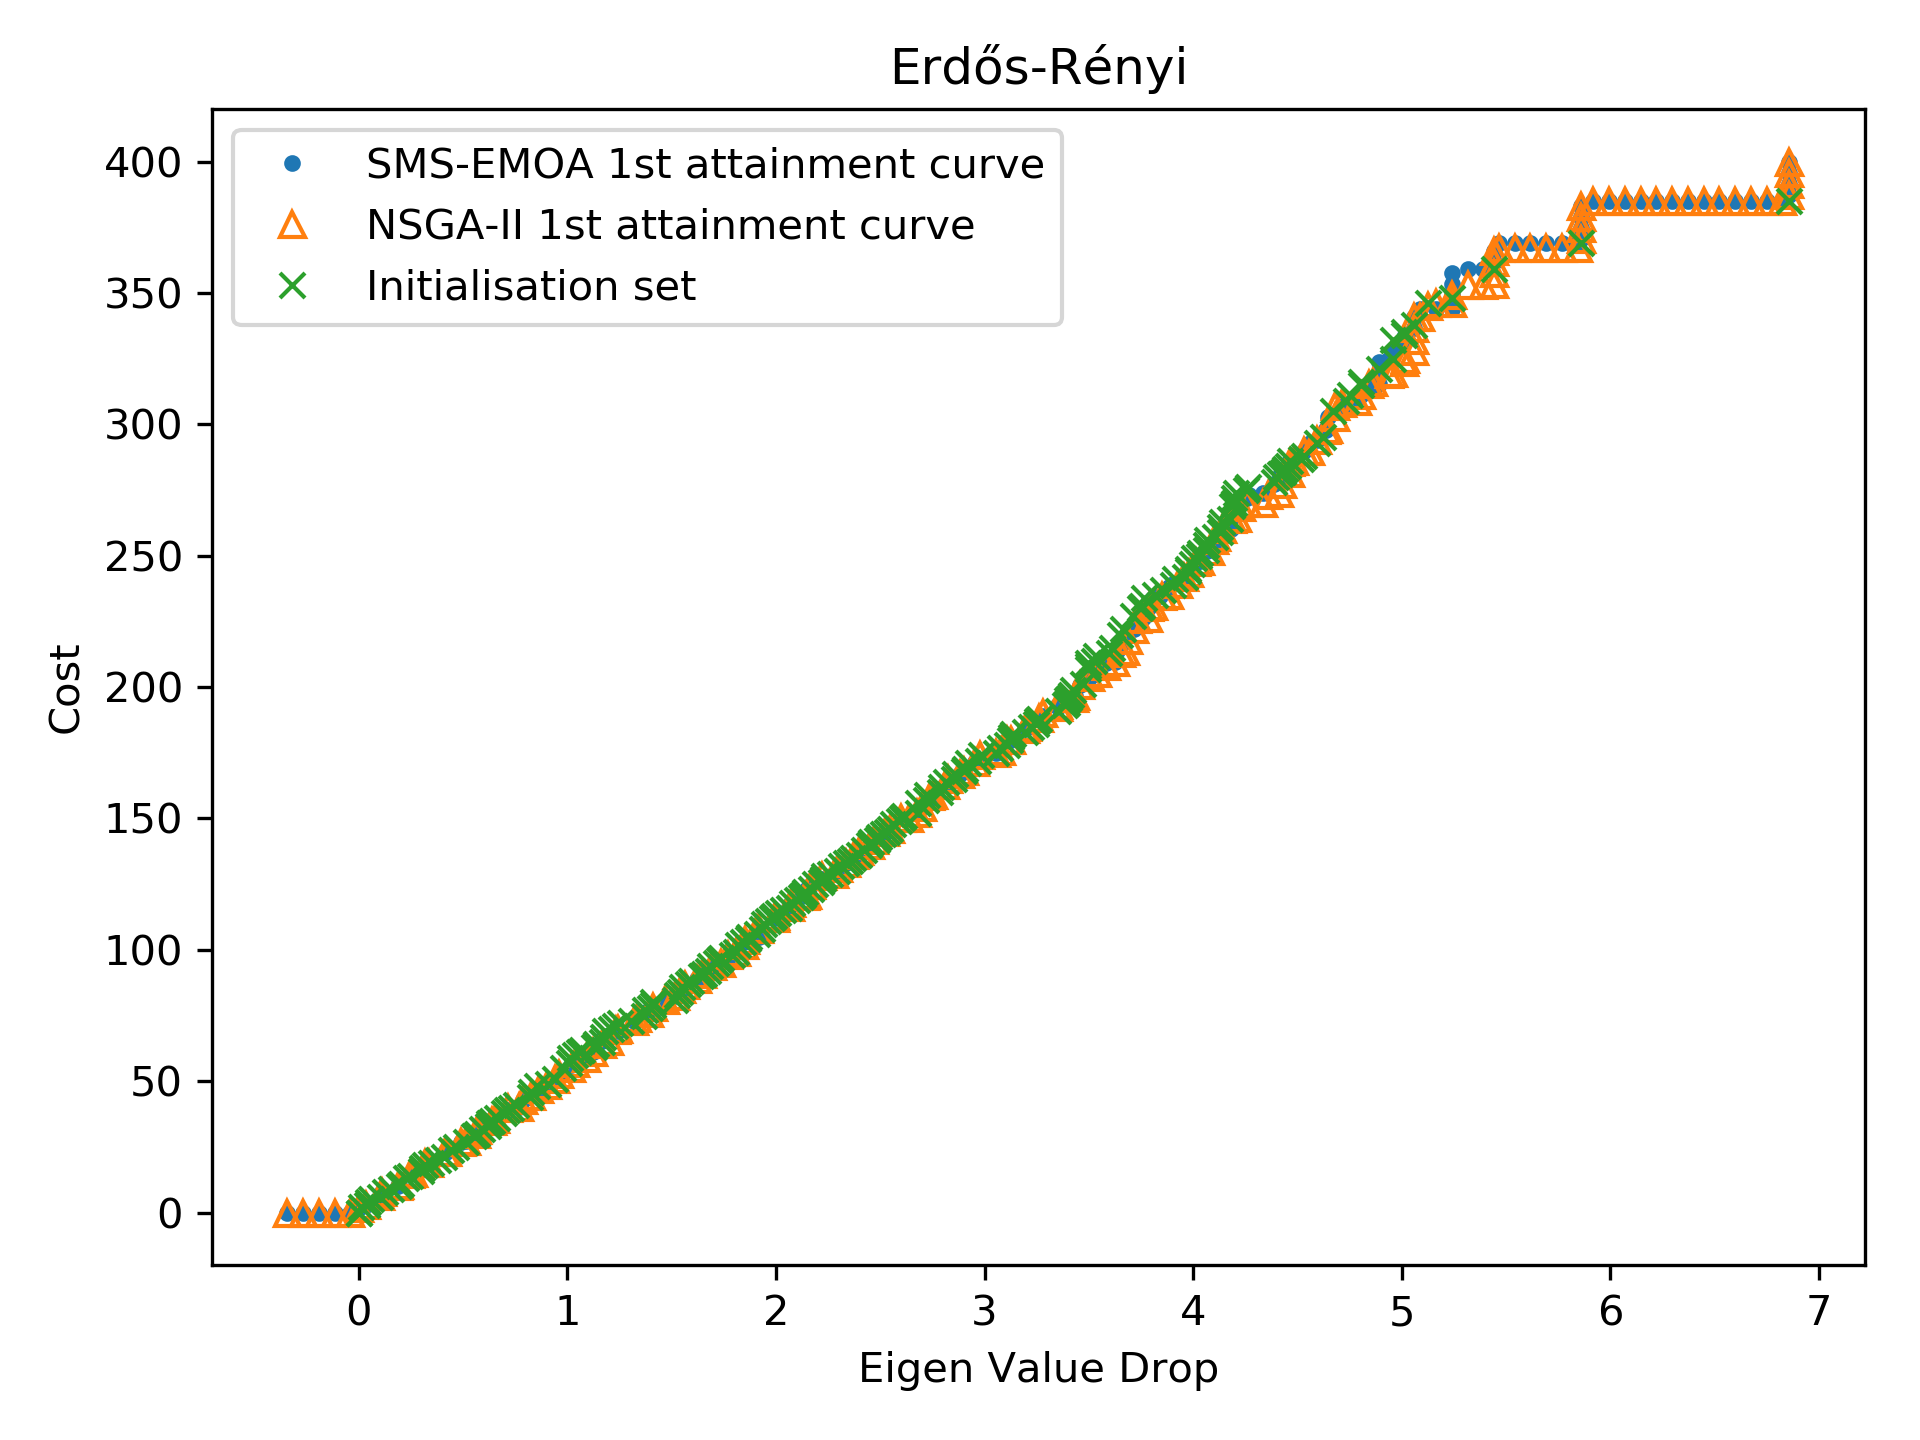
\includegraphics[width=0.75\textwidth]{results_ns_init/Erdos_Renyi_V100_attainment_nsinit}
  \caption{Pareto front approximation by the GAs and initialisation set based on NetShield and NetShield+ solutions for the Erd\H{o}s-R\'enyi graphs}
  \label{fig:erdos_renyi_atins}
\end{figure}

\begin{figure}[h!]
  \centering
    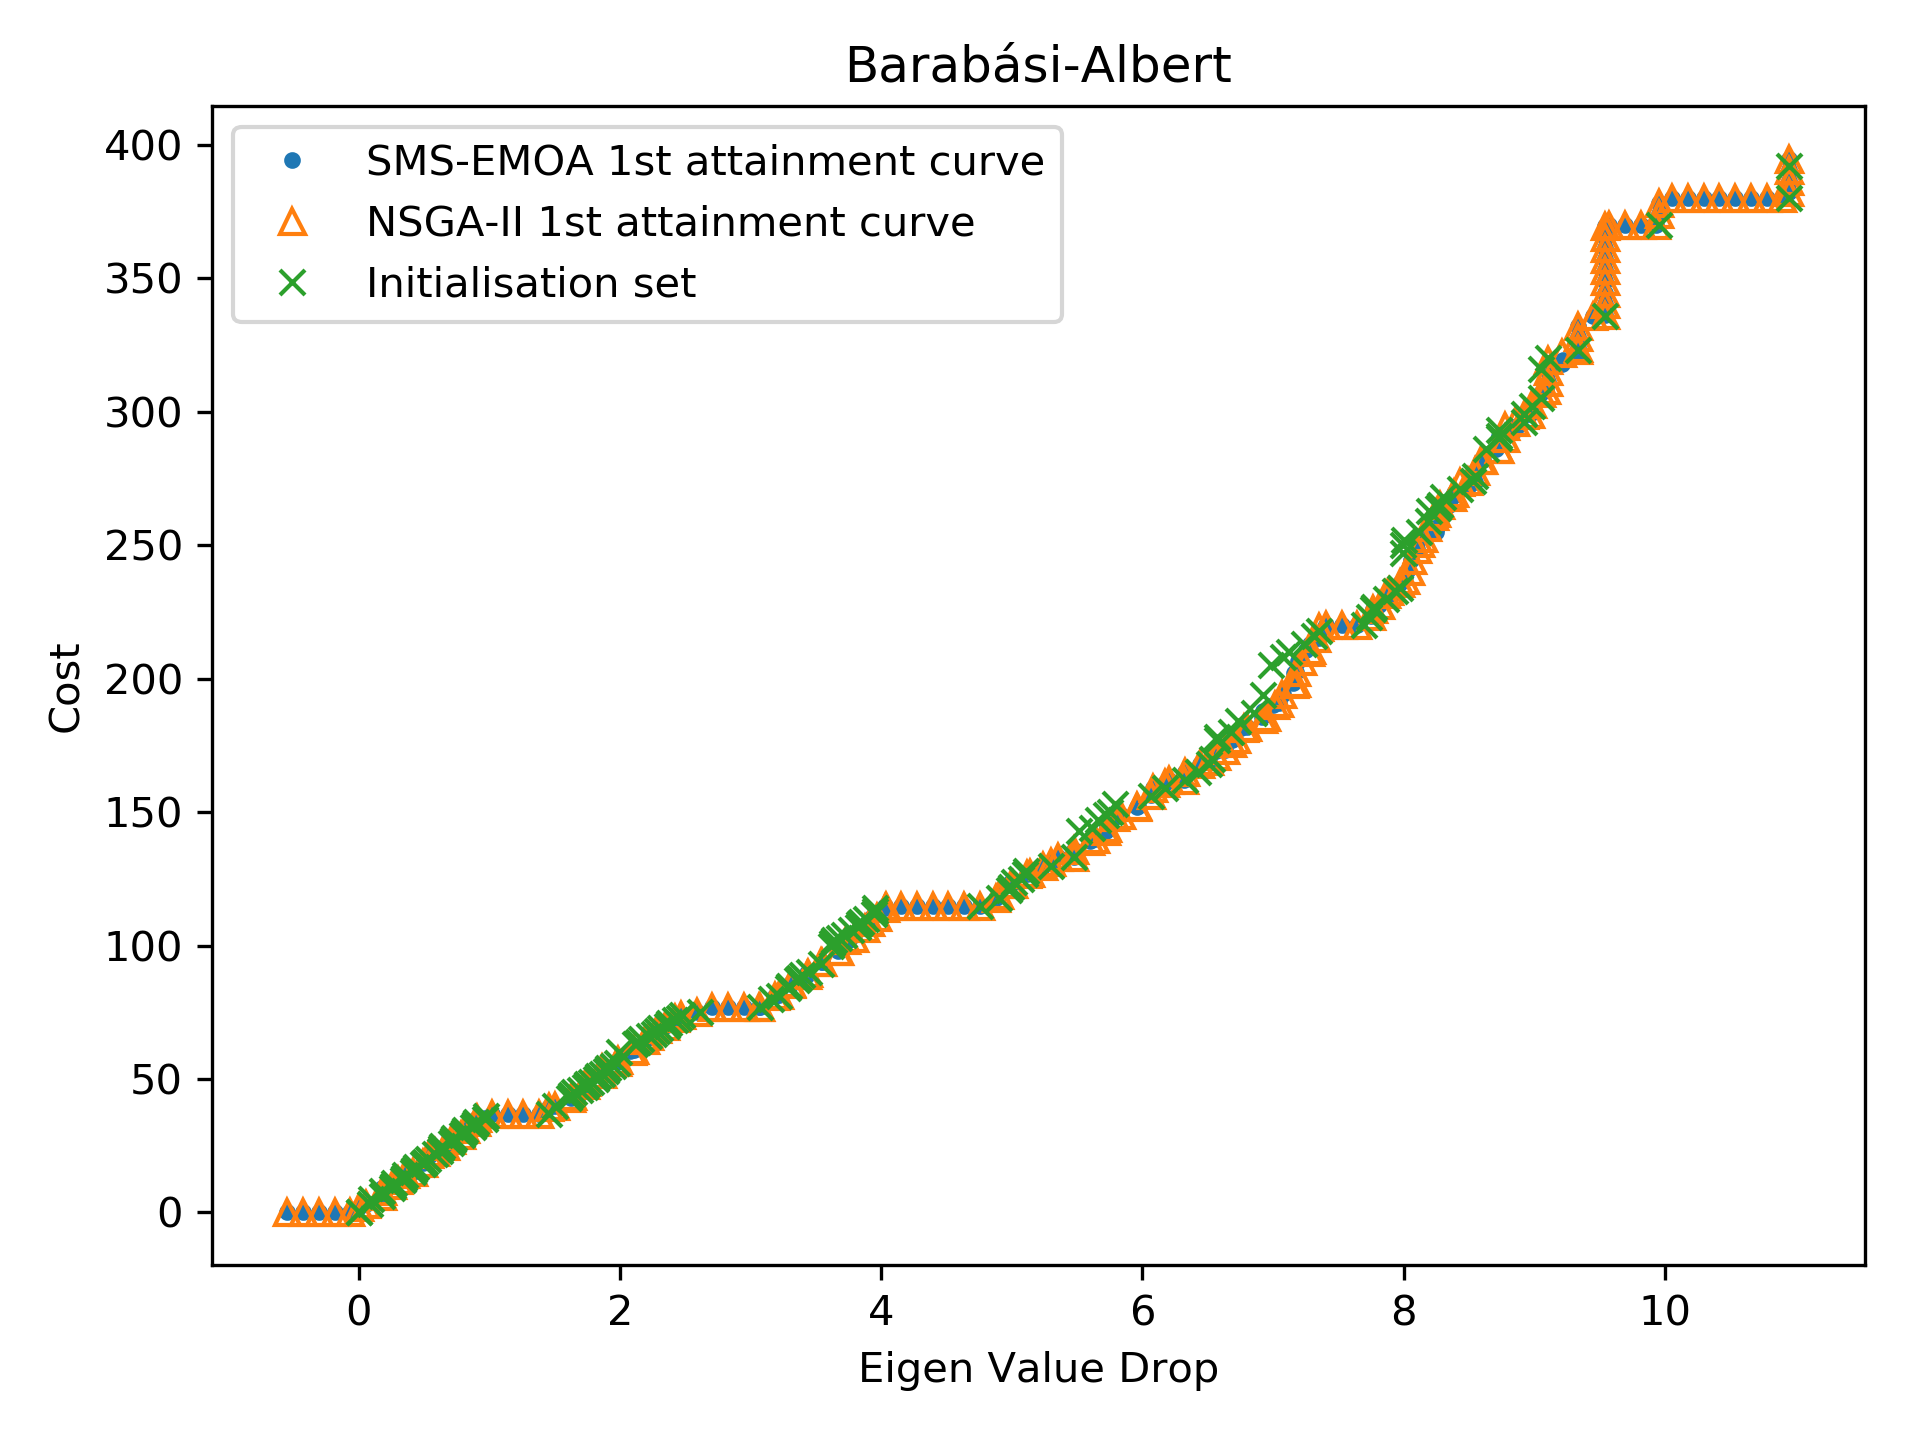
\includegraphics[width=0.75\textwidth]{results_ns_init/Barabasi_Albert_V100_attainment_nsinit}
  \caption{Pareto front approximation by the GAs and initialisation set based on NetShield and NetShield+ solutions for the Barab\'asi-Albert graph}
  \label{fig:baral_atins}
\end{figure}


\cleardoublepage


\section{Conclusion and Future Work}

The first part of this study shows, by means of enumeration and statistical sampling, that correlation can be found between the maximum eigenvalue of a graph and other graph measures, such as degree and betweenness centrality. Most of the centrality measures are correlated positively, but the correlation is not very strong. Only the Shield-value is almost perfectly correlated. This confirms, that it serves well its purpose, which is to be an approximation to the maximum eigenvalue (which is easier to optimise). Otherwise the strongest correlation found is between the average degree of nodes and the maximum eigenvalue.

The second part of the thesis gives an extended comparison between the NetShield algorithm and problem-specific genetic algorithms (GAs) for the task of dropping the eigenvalue by removing a subset of nodes of a given size $k$. While the GAs can sometimes outperform the NetShield+ algorithm for a specific graph, they appear to lose effectiveness for larger values of $k$. Using the eigen-scores of a graph to guide the search appears to run into its limits here. In addition, the GA has difficulties in solving problems on Barab\'asi-Albert model random graphs. In this case even the simple removal of the highest degree nodes provide a more effective immunisation method, which can probably be attributed to the fact that the degree distribution of Barab\'asi-Albert graphs tend to follow a power law. In addition to this, the results also show that in general maximising the eigen-drop also translate to better performance when simulating infections with continuous time Markov chains under the SIS model. This confirms that minimising the eigen-drop is also in more realistic model settings for finite size graphs a good approach for network immunisation. Although it should be noted that due to the random element of the virus spread in using this method, a bigger eigen-drop does not always guarantee better results.

The final part covers the main contribution of this thesis. In this part, it is shown that the NetShield and NetShield+ algorithms can be extended with an $\epsilon$-constraint method, using an exact quadratic programming solver (here: Gurobi). In this manner, a multi-objective variant of the node immunisation problem can be solved with a cost function added which is proportional to the effort of the node removal. The performance was mostly equivalent or better than two multi-objective genetic algorithms specifically designed for multi-objective optimisation, except for cases where the Shield-value function is not accurate enough. Combining the GAs with the NetShield algorithm as initial population only provided very marginal benefits, however. The results also show that there does not appear to be a typical shape to the Pareto fronts resulting from this problem. They are dependent on both the topology of the network and on the cost function.

If desired, future work can be done on further improving the $k$-node immunisation GA. At its best it can outperform the NetShield algorithms by considering solutions they do not yet consider. If enough improvements are made this benefit may also apply to bigger graphs and larger values of $k$.

In addition, the multi-objective approach can be researched further by adding  objectives and again test the performance of multi-objective GAs and NetShield under these scenarios. Also, no problem specific modifications were made to the multi-objective GAs. This is another possible approach to improving further Pareto front approximations.

Finally, if it is found to be possible to define the eigen-drop in a quadratic program, it would no longer be necessary to use the Shield-value function as a proxy. Then a quadratic program solver could find more accurate results. This would solve the issue of the Shield-value losing accuracy depending on the graph and size of the function input set.

It should also be noted, that we focused solely on the eigen-value drop. While this is an effective measure under the SIS infection model, the properties of real world epidemics may not be fully captured solely by this model. Such additional aspects are mentioned, for instance, in \cite{plaat}. In addition, we also assume that any nodes in the network can be immunised. This also may not translate well to real world scenarios. Therefore, future research should also take a broader view of the problem than further improving the eigen-drop via the process of node removal.

\cleardoublepage

\addcontentsline{toc}{section}{References}

\bibliographystyle{abbrv}
\bibliographystyle{unsrt}
\bibliography{bibliography}


\cleardoublepage

\counterwithin{figure}{section}
\begin{appendices}
\section{Appendix}

\subsection{Networks in data set}

The following table lists all the networks in the test data set and the number of nodes and edges in each network

\begin{center}
\begin{tabular}{ | c | c | c | }
  \hline
  Name & Nodes & Edges \\ \hline
  karate & 34 & 78 \\ \hline
  Dolphins & 62 & 159 \\ \hline
  USA & 27 & 207 \\ \hline
  Pandemic & 48 & 93 \\ \hline
  Conf. day 1 & 190 & 703 \\ \hline
  Conf. day 3 & 148 & 517 \\ \hline
  Erd\H{o}s-R\'enyi & 100 & 294 \\ \hline
  Barab\'asi-Albert & 100 & 294 \\ \hline
\end{tabular}
\end{center}

\cleardoublepage

\subsection{Network Visualisations}

The following figures contain visualisations of all networks in the data set. All nodes are scaled with their degree.

\begin{figure}[h!]
  \centering
    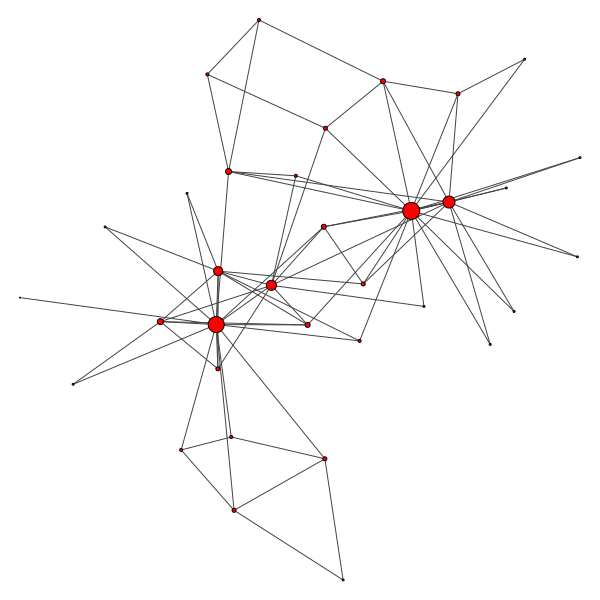
\includegraphics[width=1\textwidth]{visualisations/karate_visual}
  \caption{Karate graph}
  \label{fig:karate}
\end{figure}

\begin{figure}[h!]
  \centering
    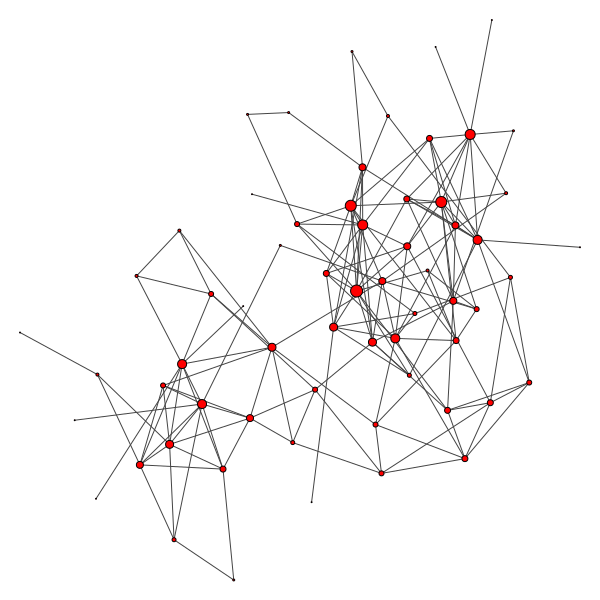
\includegraphics[width=1\textwidth]{visualisations/dolphins_visual}
  \caption{Dolphins graph}
  \label{fig:dolphins}
\end{figure}

\begin{figure}[h!]
  \centering
    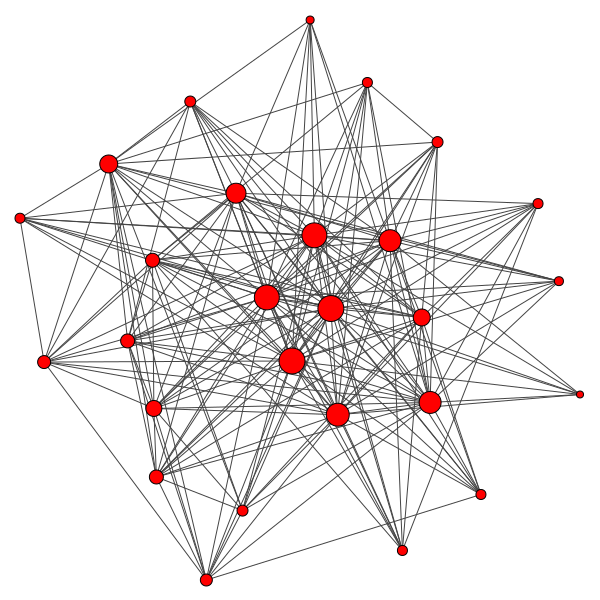
\includegraphics[width=1\textwidth]{visualisations/USA_visual}
  \caption{USA graph}
  \label{fig:USA}
\end{figure}


\begin{figure}[h!]
  \centering
    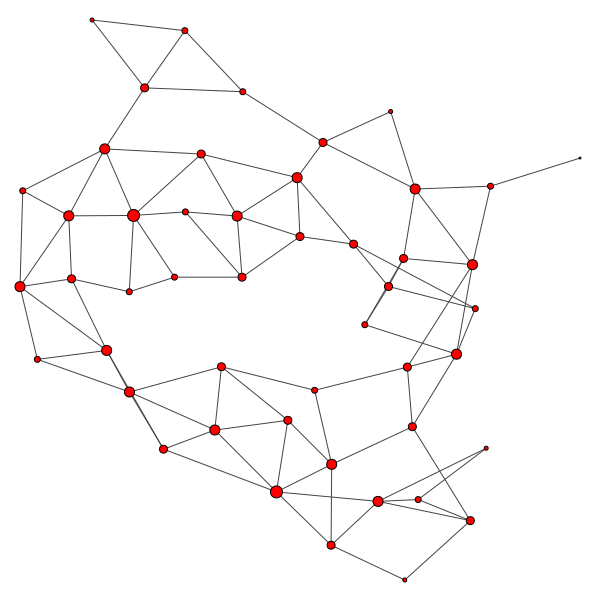
\includegraphics[width=1\textwidth]{visualisations/pandemic_visual}
  \caption{Pandemic graph}
  \label{fig:pandemic}
\end{figure}

\begin{figure}[h!]
  \centering
    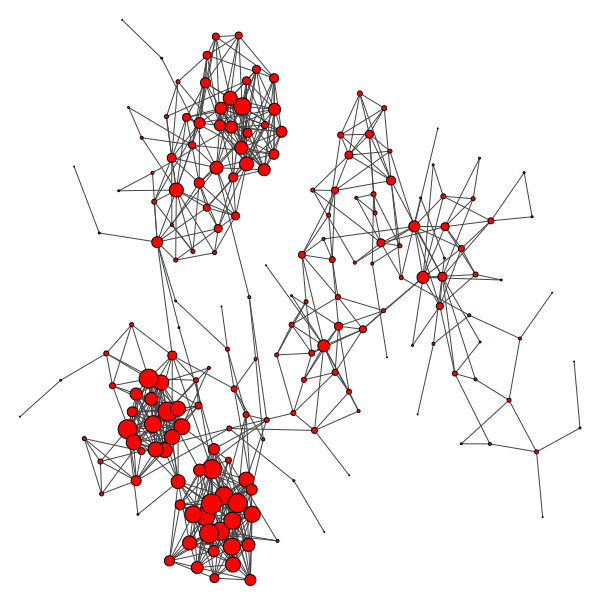
\includegraphics[width=1\textwidth]{visualisations/day1_visual}
  \caption{Conf. day 1 graph}
  \label{fig:day1}
\end{figure}

\begin{figure}[h!]
  \centering
    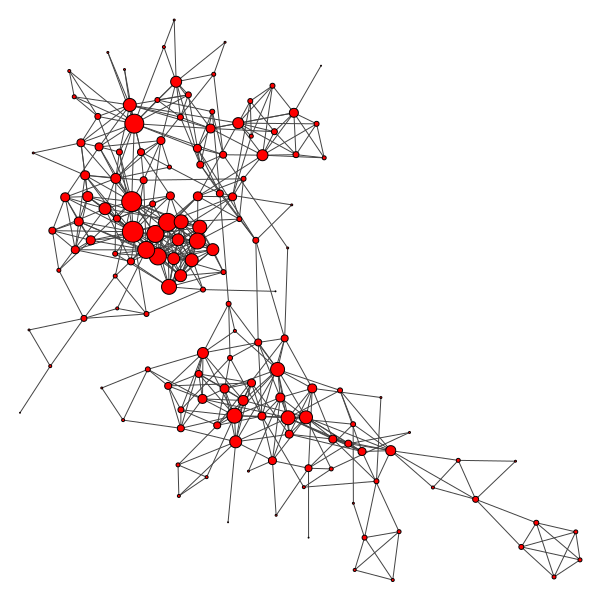
\includegraphics[width=1\textwidth]{visualisations/day3_visual}
  \caption{Conf. day 3 graph}
  \label{fig:day3}
\end{figure}

\begin{figure}[h!]
  \centering
    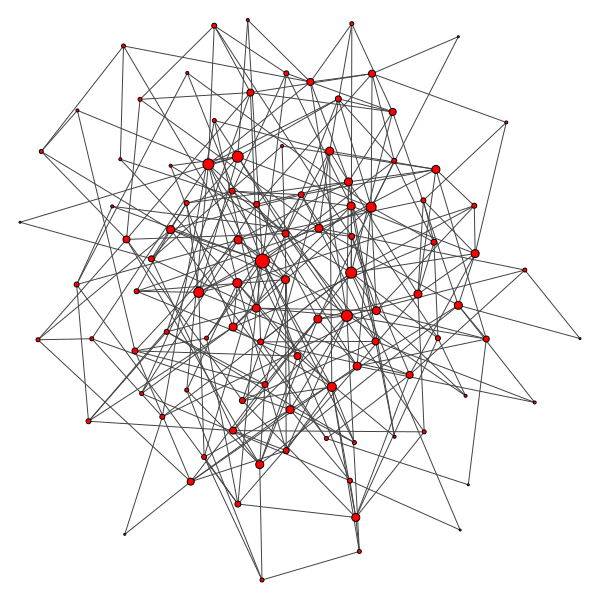
\includegraphics[width=1\textwidth]{visualisations/Erdos_Renyi_V100_visual.png}
  \caption{Sampled  Erd\H{o}s-R\'enyi graph, 100 vertices, n=294}
  \label{fig:erdosrenyi}
\end{figure}

\begin{figure}[h!]
  \centering
    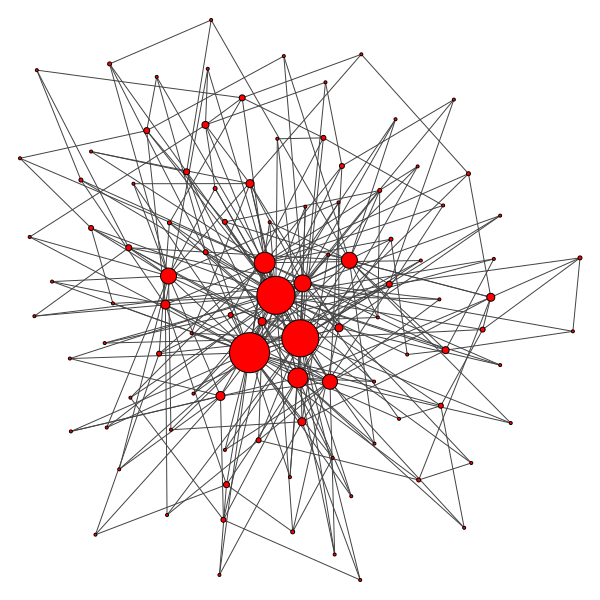
\includegraphics[width=1\textwidth]{visualisations/Barabasi_Albert_V100_visual.png}
  \caption{Sampled Barab\'asi-Albert graph, 100 vertices, m=3}
  \label{fig:barabasialbert}
\end{figure}

\end{appendices}
\end{document}
